\documentclass[10pt,letterpaper]{article}
\usepackage{jheppub}
\usepackage{physics}
\usepackage{quantikz}
\usepackage{braket}
\usepackage{tikz}
\usepackage{enumitem}
\usepackage{amsthm}
\usepackage{bbold}
\usepackage{cancel}
\usepackage{mathtools}
\usepackage{tensor}
\usepackage{multicol}
\usepackage{listings}

\usetikzlibrary{positioning}


\setlength{\parindent}{0pt}


\theoremstyle{definition}
\newtheorem{definition}{Definition}
\newtheorem{theorem}{Theorem}
\newtheorem{corollary}{Corollary}
\newtheorem{lemma}{Lemma}
\newtheorem{example}{Example}
\newtheorem{claim}{Claim}
\newtheorem{fact}{Fact}

\newcommand{\poly}{\mathrm{poly}}


%%%%%%%%%%%%%%%%%%%%%%%%%%%%%%%
% Document body
%%%%%%%%%%%%%%%%%%%%%%%%%%%%%%%

\title{\boldmath 8.371[J] Quantum Information Science II}
\author{Pamela Pajarillo}
\affiliation{Center for Theoretical Physics - Leinweber Institute, Massachusetts Institute of Technology\\ Cambridge, MA 02139, USA}
\emailAdd{pampaja@mit.edu}


\begin{document}
\maketitle

%%%%% Module  %%%%% 
%%%%% Week 1 %%%%% 
\section{Lecture 1: Introduction - 2 February 2026}
Outline:
\begin{enumerate}[label=(\Roman*)]
    \item Intro and Logistics
    \item Perspectives to Plans
    \item QM and Quantum Circuits
    \item Quantum Noise: Density Matrices
\end{enumerate}


\subsection{Lecture Perspective and Plan}
\begin{multicols}{2}
\textbf{Grading:}
\begin{enumerate}
  \item Homework: 15\%
  \item Participation: 10\%
  \item Project: 15\%
  \item Quizzes: 60\%
\end{enumerate}
\columnbreak
\textbf{Four units}
\begin{enumerate}
  \item Quantum Error Correction
  \item Quantum Algorithms
  \item Models of Fault Tolerant Quantum Computing
  \item Entanglement
\end{enumerate}
\end{multicols}
Goal: Be able to write research-quality papers\\
Schedule: 4 Modules - each with 1 quiz in class, 3 TPS (Think-Pair-Share)



\subsubsection{Quantum Error Correction (QEC)}
Encode: $a\ket{0} + b\ket{1} \mapsto a \ket{0_L} + b \ket{1_L}$ \\
What?: 
\begin{itemize}
    \item Method for reversing decoherence (quantum noise)
    \item Hiding from noise
    \item Controlling entropy
\end{itemize}
How?:
\begin{itemize}
    \item Embed our system into a larger system (embed into a larger Hilbert space)
    \item ``Church of the larger Hilbert space''
\end{itemize}
Why?:
\begin{itemize}
    \item In order to make quantum computing a reality, we have to deal with noise
    \item Security of Quantum Key Distribution
    \item Black Holes
\end{itemize}
Unknown?:
\begin{itemize}
    \item Efficiency: (how large of a system do we need to use to embed a small system in order to deal with the noise that we have) rates, overhead
    \item Given a code, is it locally testable? If so, we can prove the Probabilistically Checkable Proofs (PCP) theorem 
\end{itemize}



\subsubsection{Quantum Algorithms}
We can picture a quantum algorithm as something that takes in an input $x$ that encodes some kind of function and gives some output.  \\
\begin{center}
\begin{quantikz}
    & \gate[3]{U} & \\
    \lstick{$x$} & & \\
    & & 
\end{quantikz}
\end{center}
What?:
\begin{itemize}
    \item Mapping of problems onto quantum resources 
\end{itemize}
How?
Toffoli gate: output is Z XOR (X AND Y) This is universal for all reversible computation and all classical computation. Since this is a unitary gate
\begin{center}
    \begin{quantikz}
    \lstick{$x$} & \ctrl{2} & \\
    \lstick{$Y$} & \ctrl{1} & \\
    \lstick{$Z$} & \targ{} & \rstick{$Z \oplus XY$}\\
    \end{quantikz}
\end{center}

\begin{itemize}
    \item Reversible Quantum Computation
    \item Quantum Search
    \item Quantum Fourier Transform (QFT) $\rightarrow$ Factoring, Phase Estimation $HHL$ ($A\vec{x} = \vec{b}$)
    \item Quantum Simulation
    \item Grand unification of Quantum Algorithms: Quantum Singular Value Transform (Quantum signal processing)
\end{itemize}

Why?
\begin{itemize}
    \item Reveal the nature of mathematical problems (polynomial hierarchy)
    \item Nature of physical world (easy/hard)? 
    \item Practical applications (quantum computational sensing)
\end{itemize}

Unknowns?
\begin{itemize}
    \item When is quantum better than classical? (Quantum advantage)
    \item What is the hardness relative to noise? 
    \item what are hard/easy quantum transforms?
\end{itemize}

\subsubsection{Fault Tolerant Quantum Computing}
What?: 
\begin{quantikz}
    & \gate[3]{U} & \gate[3]{QEC} & \\
    \lstick{$x$} & & &\\
    & & &
\end{quantikz}
%\gategroup[3,steps=2,style={dashed,rounded corners}

What?:
\begin{itemize}
    \item Make reliable quantum systems from unreliable components (a human is an example)
\end{itemize}
How? 
\begin{itemize}
    \item von Neumann - compute on codes 
    \item Measurement induces change in the quantum systems $\rightarrow$ measurement-based computation
    \item Teleportation-based quantum computation
\end{itemize}
Why?
\begin{itemize}
    \item Useful quantum computation
    \item New physics?
    \item The transition between faulty $\leftrightarrow$ reliable is a phase transition; Fault tolerant threshold
\end{itemize}
Unknowns:
\begin{itemize}
    \item Fault tolerant threshold
    \item FTQC $\Leftrightarrow$ PICP (Probabilistically Checkable Proofs)
\end{itemize}



\subsubsection{Entanglement}
What?
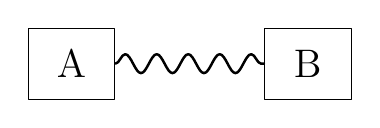
\begin{tikzpicture}[line cap=round, line join=round]

% Boxes
\node[draw, minimum width=1.1cm, minimum height=0.9cm] (A) at (0,0) {\Large A};
\node[draw, minimum width=1.1cm, minimum height=0.9cm] (B) at (3,0) {\Large B};

% Wavy connection
\draw[decorate, decoration={snake, amplitude=1.2mm, segment length=4mm}, line width=0.9pt]
  (A.east) -- (B.west);

\end{tikzpicture}
\begin{itemize}
    \item A new kind of physical resource
    \item Multi-party protocols
    \item Shared secret, communication
\end{itemize}
How?:
\begin{itemize}
    \item Non-local operators
    \item Communication bits $\rightarrow$ qubits
    \item Quantum measurement is akin to a one-way function
\end{itemize}
Why?:
\begin{itemize}
    \item No exponential quantum advantage without entanglement
    \item Provable exponential quantum communication advantage over classical 
    \item MIP$^{*}$ = RE, MIP = multiple provers, RE = recursively enumerable 
\end{itemize}
Unknowns?:
\begin{itemize}
    \item multi-partite entanglement
    \item entanglement + noise tends to destroy
\end{itemize}


\subsection{Quantum Mechanics and Quantum Circuits}
Four postulates:
\begin{itemize}
    \item State: system = unit vector $\ket{\psi}$ 
    \item Gate: $\ket{\psi'} = U \ket{\psi}$ 
    \item Measurement: $\{m_k\}$ s.t. $\sum_k m_k^\dagger m_k = I$ (completeness theorem); when measured $\ket{\psi}$ collapses $\ket{\psi} \mapsto \frac{m_k\ket{\psi}}{\sqrt{p_k}}$, where $p_k = \braket{\psi|m_k^\dagger m_k|\psi}$
    \item Composition: Tensor (Kronecker) Product 
\end{itemize}
Quantum Circuits:
\begin{itemize}
    \item Qubit 
        \begin{quantikz}
            & \qwbundle{} & 
        \end{quantikz}
    \item Bit
        \begin{quantikz}
            & \setwiretype{c} & 
        \end{quantikz}
    \item Gates
        \begin{quantikz}
            & \gate{U} & 
        \end{quantikz}
    \item Entangled States
        \begin{quantikz}
            \makeebit{} & & \\
            & &
        \end{quantikz}
\end{itemize}
Solovay-Kitaev Theorem: tells us how difficult it is to construct a given unitary gate $U$. The difficulty can be quantified. The quantification depends on the set of gates to construct. For a single qubit, we can construct any $U$ from $H,T$ \\
Solovay-Kitaev: any single qubit gate can be described by a string of $H$ and $T$ gates ( with each addition gate doubles the precision, $H$ and $T$ are like binary matrix digits) \\  
\begin{quantikz} & \gate{U} &\end{quantikz} $\doteq$ \begin{quantikz} & \gate{H} &\end{quantikz} $H = \frac{1}{\sqrt{2}}\begin{pmatrix}1 & 1 \\ 1 & -1\end{pmatrix}$, \\
\hspace*{2.3cm}\begin{quantikz} & \gate{S} &\end{quantikz} $ S = \sqrt{Z} = \frac{1}{\sqrt{2}}\begin{pmatrix}1 & 0 \\ 0 & i\end{pmatrix}$\\
\hspace*{2.3cm}\begin{quantikz} & \gate{T} &\end{quantikz} $ T = \sqrt{S} = \frac{1}{\sqrt{2}}\begin{pmatrix}1 & 0 \\ 0 & e^{i\frac{\pi}{4}}\end{pmatrix} \leftarrow \frac{\pi}{8}$ gate  \\
$H, T$ and $CNOT$ gives us all universal


\subsection{Quantum Noise and Density Matrices}
Motivation Question: Given $\ket{\psi}$ or $\phi$ with probability $\frac{1}{2}$. What state? $\rho = \frac{1}{2}\ketbra{\psi}{\psi} + \frac{1}{2} \ketbra{\phi}{\phi}$ 

\begin{definition}
    A matrix $\rho$ is a density matrix iff a) $\Tr \rho = 1$, b) $\rho \geq 0$ i.e. $\forall \ket{\phi}$, $\braket{\phi|\rho|\phi} \geq 0$ and real ($\rho$ is positive definite and Hermitian)
\end{definition}

\begin{claim}
    $\rho = \sum p_k \ketbra{\psi_k}$, where $p_k$ are probabilities and sum to 1, is a legal density matrix. \\
     $\Tr \rho = 1$ and $\braket{\phi|\rho|\phi} = p_k \braket{\phi|\psi_k} \braket{\psi_k|\phi}$
\end{claim} 

\begin{claim}
    Any $\rho$ can be expressed as $\rho = \sum_k p_k \ketbra{\psi_k}{\psi_k}$ where $\sum_k p_k = 1$. (Proof by spectral decomposition: $p_k$ are eigenvalues and $\ket{\psi}$ are eigenvectors)
\end{claim}

\begin{definition}
    A density matrix $\rho$ is pure iff $\rho = \ketbra{\psi}$
\end{definition}

\begin{example}
    Is $\rho = p_k \rho_k$ a legal density matrix? Yes\\
    Is $\rho = \frac{1}{2}\begin{pmatrix}1 & 0 & 0 & 0 \\ 0 & 0 & 1 & 0 \\ 0 & 1 & 0 & 0 \\ 0 & 0 & 0 & 1 \end{pmatrix}$ a legal density matrix? No, because the block in the middle is the $X$ matrix $\begin{pmatrix}0 & 1 \\ 1 & 0 \end{pmatrix}$, which have eigenvalues $\pm 1$.  
\end{example}

\begin{lemma}
    von Neumann unravellings: \\
    Let $\rho = \sum p_k \ketbra{\psi_k}$. Then $\rho = \rho' = \sum_i q_i \ketbra{\phi_i}$, where $\ket{\psi}$  and $\ket{\phi}$ iff $\sqrt{p_k} \ket{\psi_k} =  \sum_j U_{kj} \ket{\phi_j}$
\end{lemma}
If a density matrix is not legal, it cannot describe a physical system. Otherwise, any density matrix can be physically realized if it is a legitimate density matrix. (1-1 with physical reality) 

\begin{example}
    Suppose $\rho = \frac{1}{2} \begin{pmatrix}1 & 0 \\ 0 & 1\end{pmatrix} = \frac{1}{2} \ketbra{0} + \frac{1}{2} \ketbra{1} = \frac{1}{2} \ketbra{+} + \frac{1}{2} \ketbra{-}$     
\end{example}
Avoid preferred ensemble fallacy!
\section{Lecture 2: Quantum Operations - 4 February 2026}
Outline: 
\begin{enumerate}[label=(\Roman*)]
    \item System-environment model
    \item Definition: Quantum Operations
    \item Operator sum representation (OSR)
    \item OSR is not unique
    \item First look: quantum error detection
\end{enumerate}
Last time: Density matrix $\rho = \sum_k p_k \ketbra{\psi_k}$ or pure states  


\subsection{System-environment model}
Hilbert spaces: 
\begin{itemize}
    \item $\mathcal{H}$: the one we care about
    \item $\mathcal{G}$: environment
\end{itemize}

\begin{center}
\begin{tabular}{ c | c }
Object & Lives in/on  \\
\hline
$\ket{\psi}$ & $\mathcal{H}$  \\  
$\ket{e}$ & $\mathcal{G}$  \\  
$\ket{\Phi}$ & $\mathcal{G} \otimes \mathcal{H}$   \\  
$E_k$ & $\mathcal{G} \otimes \mathcal{H}$   \\  
\end{tabular}
\end{center}

\begin{center}
\begin{quantikz}
    \lstick{$\ket{\psi}$ or $\rho_{in}$} & \gate[2]{U} & \rstick{$\rho_{out}$? } \\
    \lstick{$\ket{e}$} &  & \meter{}
\end{quantikz} 
\end{center}
Claim: From the ``church of the larger Hilbert space", this structure can model can essential model anything you can do to a quantum system, i.e. black box included \\
This environment corresponds to the entire universe, something we don't have control over, so we're actually not measuring, but it is a useful mathematical tool (measurement gets thrown away). \\
\begin{equation}
    \ket{\psi} \otimes \ket{e} \rightarrow \underbrace{U [\ket{\psi} \otimes \ket{e}]}_{\ket{\Phi}} = 
\end{equation}
When we measure, we can pick some basis $\ketbra{e_0}, \ketbra{e_1}, \ldots$, then $\rho_{out}$ possible measurements:
\begin{align}
    [\bra{e_0} \otimes & \mathbb{1}] \ket{\Phi} \\ 
    [\bra{e_1} \otimes & \mathbb{1}] \ket{\Phi} \\ 
    &\vdots
\end{align}
The density matrix $\ket{\rho_{out}}$ 
\begin{equation}
    \rho_{out} = \sum_k (\bra{e_k} \otimes \mathbb{1}) \ketbra{\Phi} (\ket{e_k} \otimes \mathbb{1})
\end{equation}
But we don't have control over the environment, and we don't even know the input $\ket{e}$ and the measurement basis. Ideally, we want to get rid of the environment. 
\begin{align}
    [\bra{e_k} \otimes \mathbb{I}) \ket{\Phi}] &= [\bra{e_k} \otimes \mathbb{I}] U [\ket{e} \otimes \ket{\psi}] \\
    &= \underbrace{[\bra{e_k} \otimes \mathbb{I}] U [\ket{e} \otimes \mathbb{I}]}_{\text{projecting to }\mathcal{H}} \underbrace{\ket{\psi}}_{\mathcal{H}}
\end{align}
Because we're multiplying by states in $\mathcal{G}$ on both sides, we're projecting down to $\mathcal{H}$
Let us define
\begin{equation}
    E_k = [\bra{e_k} \otimes \mathbb{I}] U [\ket{e} \otimes \mathbb{I}]
\end{equation}
Now we can the possible states of $\rho_{out}$ to be 
\begin{align}
    E_0 &\ket{\Phi} \\ 
    E_1 &\ket{\Phi} \\ 
    &\vdots
\end{align}
The expression for $\rho_{out}$ is
\begin{equation}
    \rho_{out} = \sum_k E_k \ketbra{\psi}E_k^\dagger 
\end{equation}
If we substitute the input $\ket{\psi}$ to $\rho_in$, then 
\begin{equation}
    \rho_{out} = \sum_k E_k \rho_{in} E_k^\dagger 
\end{equation}
$E_k$ is not unitary. It is a fact that 
\begin{equation}
    \sum_k E_k^\dagger E_k = \mathbb{1}
\end{equation}
This can be shown by first calculating $E_k^\dagger$,
\begin{equation}
    E_k^\dagger = (\bra{e} \otimes I ) U^
    \dagger (\ket{e_k} \otimes I )
\end{equation}
Then
\begin{equation}
    E_k^\dagger E_k = (\bra{e} \otimes \mathbb{1} ) U^
    \dagger (\ket{e_k} \otimes \mathbb{1}) (\ket{e_k} \otimes \mathbb{1}) U  (\bra{e} \otimes \mathbb{1} )
\end{equation}
Combining the middle terms, $(\ket{e_k} \otimes I) (\bra{e_k} \otimes \mathbb{1}) = \ketbra{e_k} \otimes \mathbb{1}$. Then summing over $k$,
we have that 
\begin{equation}
    \sum_k \ketbra{e_k} \otimes \mathbb{1} = \mathbb{1} \otimes \mathbb{1}
\end{equation}
Then, 
\begin{align}
    \sum_k E_k^\dagger E_k &= (\bra{e} \otimes \mathbb{1} ) U^
    \dagger (\ket{e_k} \otimes \mathbb{1}) (\ket{e_k} \otimes \mathbb{1}) U  (\bra{e} \otimes \mathbb{1} ) \\
    &= (\bra{e} \otimes \mathbb{1} ) U^
    \dagger U \ket{e} \otimes \mathbb{1} \\
    & = \mathbb{1}_{\mathcal{H}}
\end{align}
The dimension of $\mathcal{G}$ does not need to be bigger than $\mathcal{H}$ because if we have a maximally entangled state in $\mathcal{H}$ there are extra dimensions in $\mathcal{G}$ that will not be used.\\
Without loss of generality we can take $\ket{e} = \ket{0}$. \\
Density matrices are just tools to be able to throw away parts of the Hilbert space we don't want. 


\subsection{Definition: Quantum Operation (channels)}
Quantum channels should be the most general thing you can do to a quantum system. ``Things that transform mixed states into mixed states" (we need a valid output density matrix). Density matrices must have $Tr(\rho) = 1$. \\
Let $\mathcal{E}$ be a generic quantum operation, then we must have $Tr(\mathcal{\rho}) = 1$.\\
If $\rho_a,\rho_b$ are density matrices, and let $\alpha,\beta > 0$, $\alpha\rho_a + \beta\rho_b$ is a density matrix (up to normalization). This implies that $\mathcal{E}[\alpha\rho_a + \beta\rho_b] = \alpha \mathcal{E}(\rho_a) + \beta \mathcal{E}(\rho_b)$. \\
Positive-semidefinite: all eigenvalues are greater than 0 (any principle minor must have positive determinant). Additionally, if we have $\ket{\psi} = \sum_i \alpha_i \ket{i}$, then $\ketbra{\psi} = \alpha_i^* \alpha^i$ must be a real non-negative number. We must have positive semidefinite in order for it to make sense physically. \\
$\mathcal{E}$ must be a ``completely positive" map, which means it keeps things positive-semidefinite. 

\begin{example}
    Suppose we have 
    \begin{equation}
        \rho = \begin{pmatrix}
            a & b \\ d & c
        \end{pmatrix}
    \end{equation}
    Example of wrong math: Is 
    \begin{equation}
        \mathcal{E}(\rho) = \begin{pmatrix}
            a & d \\ b & c
        \end{pmatrix}
    \end{equation}
    a legal map? No.\\
    Just any $\rho \rightarrow \mathcal{E}(\rho)$ remaining positive semi definite is not enough for complete positivity. \\
    $\mathcal{E}$ is currently on 1 qubit. \\
    Let's consider $ \mathbb{1} \otimes \mathcal{E}$ and $\ket{\psi} = \ket{00} + \ket{11}$. Then 
    \begin{equation}
        \ketbra{\psi} = \begin{pmatrix}
            1 & 0 & 0 & 1 \\
            0 & 0 & 0 & 0 \\
            0 & 0 & 0 & 0 \\
            1 & 0 & 0 & 1 
        \end{pmatrix}
    \end{equation}
    Then
    \begin{equation}
        (\mathbb{1} \otimes \mathcal{E}) \ketbra{\psi} = \begin{pmatrix}
            1 & 0 & 0 & 0 \\
            0 & 0 & 1 & 0 \\
            0 & 1 & 0 & 0 \\
            0 & 0 & 0 & 1 
        \end{pmatrix}
    \end{equation}
    i.e. if we tensor product it with some external system, it also needs to be positive semi-definite. This is also true in any generalization $\ket{\psi}= \sum_i^d \ket{i}\otimes \ket{i}$. \\ 
    Physics intuition: suppose we have two mixed states $\rho$ and $\phi$, and we applied $\mathcal{E}$ to $\rho$, the entire system must still be quantum. 
\end{example}

The system-environment model and quantum operations are equivalent. The system-environment model captures everything in quantum operations in a strict way. i.e. anything we can write down in particular using
\begin{equation}
    \rho_{out} = \sum_k = E_k\rho_{in}E_k^\dagger \qquad \sum_k E_k^\dagger E_k = \mathbb{1}
\end{equation}
These $E_k$'s are not unique (i.e. measurement basis can be different - we can insert a unitary $V$ before we make a measurement). 
\begin{center}
\begin{quantikz}
    \lstick{$\rho_{in}$} & \gate[2]{U}&  & \rstick{$\ket{\rho_{out}}$? } \\
    \lstick{$\ket{e}$} & & \gate{V} & \meter{}
\end{quantikz} 
\end{center}

$E_k$'s are called Krauss operators. \\
Let $F_j$ be the new Krauss operators. Then
\begin{equation}
    F_j = \sum_k V_{jk} E_k
\end{equation}

\begin{example}
    Suppose 
    \begin{center}
    \begin{quantikz}
        \lstick{$\rho_{in}$} & \gate[]{U}&   \rstick{$\ket{\rho_{out}}$ } \\
        \lstick{$\ket{e}$} & &      
    \end{quantikz} 
    \end{center}
    The Krauss operator is $E_0 = 0$ because output is $U \rho_{out} U^\dagger$. \\
\end{example}

\begin{example}
    Suppose $\{\Pi_i\}$ are a set of projectors.
    \begin{center}
    \begin{quantikz}
        \lstick{$\rho_{in}$} & \meter{\Pi_i}&   \rstick{$\ket{\rho_{out}}$ } \\
        \lstick{$\ket{e}$} & &      
    \end{quantikz} 
    \end{center}
    But we don't look at the measurement outcome (black box). The Krauss operator is ${E_k} = {\Pi_i}$. Now let's look at
    \begin{center}
    \begin{quantikz}
        \lstick{$\rho_{in}$} & \ctrl{1}&   \rstick{$\ket{\rho_{out}}$ } \\
        \lstick{$\ket{0}$} & \gate{} &      
    \end{quantikz} 
    \end{center}
    where the gate is a unitary operation $U$. Suppose 
    \begin{equation}
        \Pi_i = \ketbra{\psi_k}
    \end{equation}
    where $\ket{\psi_k}$ lives on $\mathcal{H}$. Then 
    \begin{equation}
        U \ket{\psi_k} \ket{0} \rightarrow \ket{\psi_k} \ket{\psi_k}
    \end{equation}
    if we measure, we'll be projecting on whatever $\ket{\psi_k}$ is.
\end{example}

\begin{claim}
    Suppose
    \begin{equation}
        E_0 = \begin{pmatrix}
            1 & 0 \\ 0 & \sqrt{1 - \lambda} 
        \end{pmatrix} \quad E_1 = \begin{pmatrix}
            0 & 0 \\ 0 & \sqrt{\lambda}
        \end{pmatrix}
    \end{equation}
    These are phase dampening channel. For intuition, if we have some arbitrary density matrix, 
    \begin{equation}
        \rho = \begin{pmatrix}
            a & b \\ b^* & c
        \end{pmatrix} \mapsto \begin{pmatrix}
            a & \sqrt{1 - \lambda} b \\ \sqrt{1 - \lambda} b^* & c
        \end{pmatrix}
    \end{equation}
\end{claim}
\section{PSet 1 - 8 February 2025}
\subsection{Problem 1 - Two qubit state creation in python cirq}
\begin{center}
\begin{quantikz}[slice all, remove end slices=1,slice
titles=slice \col,slice style=blue,slice label style
={inner sep=1pt,anchor=south west,rotate=40}]
\lstick{$\ket{0}$} & \gate{R_y(\theta)} & \ctrl{1} & \qw & \qw \\
\lstick{$\ket{0}$} &                    & \targ{} & \qw  & \qw
\end{quantikz}
\end{center}
Find $\theta$ such that the quantum circuit creates the state 
\begin{equation}
    \sqrt{\frac{3}{4}}\ket{00} + \sqrt{\frac{1}{4}}\ket{11}
\end{equation}
$R_y(\theta)$ is given by 
\begin{align}
    R_y(\theta) &= e^{i \frac{\theta}{2} Y} \\
    &= \cos\frac{\theta}{2} \mathbb{1} - i \sin \frac{\theta}{2} Y \\
    &= \cos\frac{\theta}{2} \begin{pmatrix} 1 & 0 \\ 0 & 1 \end{pmatrix} - i \sin \frac{\theta}{2} \begin{pmatrix} 0 & -i \\ i & 0\end{pmatrix}\\
    &= \begin{pmatrix} \cos{\frac{\theta}{2}} & 0 \\ 0 &  \cos{\frac{\theta}{2}} \end{pmatrix} + \begin{pmatrix} 0 & - \sin \frac{\theta}{2} \\ \sin \frac{\theta}{2} & 0 \end{pmatrix} \\
    &= \begin{pmatrix} \cos \frac{\theta}{2} & - \sin \frac{\theta}{2} \\ \sin \frac{\theta}{2} & \cos \frac{\theta}{2}\end{pmatrix}
\end{align}
Our initial state is $\ket{00}$. Applying the $R_y$ gate to the first qubit,
\begin{equation}
    R_y(\theta)\ket{0} = \cos \frac{\theta}{2}\ket{0} + \sin \frac{\theta}{2}\ket{1}
\end{equation}
At slice 1,
\begin{equation}
    \cos \frac{\theta}{2}\ket{00} + \sin \frac{\theta}{2}\ket{10}
\end{equation}
At slice 2,
\begin{equation}
    \cos \frac{\theta}{2}\ket{00} + \sin \frac{\theta}{2}\ket{11}
\end{equation}
Now we need to match coefficients
\begin{equation}
    \cos \frac{\theta}{2} = \frac{\sqrt{3}}{2} \text{ and } \sin \frac{\pi}{2} = \frac{1}{2}
\end{equation}
Therefore
\begin{equation}
    \frac{\theta}{2} = \frac{\pi}{6} \Rightarrow \boxed{\theta =\frac{\pi}{3}}
\end{equation}

The cirq code is then given as: 
\begin{lstlisting}
    def run():
    q0, q1 = cirq.LineQubit.range(2)    # Define qubits
    theta = np.pi/3    # CHANGE ME (numpy as imported as np)
    
    # Create the circuit
    circuit = cirq.Circuit(
        cirq.ry(theta)(q0),    # Apply Ry gate to q0 to get desired amplitudes
        cirq.CNOT(q0, q1)      # Apply CNOT to entangle q0 and q1
    )
    
    print("Circuit being used to create the desired state:\n", circuit)

    simulator = cirq.Simulator()
    result = simulator.simulate(circuit)
    print("State vector of the created state:")
    print(np.round(result.final_state_vector, 5))
    return(result.final_state_vector.tolist())

\end{lstlisting}

\newpage
\subsection{Problem 2 - Density matrices and unravelings}
Consider the bipartite state 
\begin{equation}
    \ket{\psi_{AB}} = \sqrt{\frac{3}{4}}\ket{00} + \sqrt{\frac{1}{4}}\ket{11}
\end{equation}
Suppose Bob measures in the computational basis. \\
If Bob measures $\ket{0}$, 
\begin{align}
    (\mathbb{1} \otimes \ketbra{0}{0}) \ket{\psi_{AB}} = \sqrt{\frac{3}{4}}\ket{00}
\end{align}
Therefore, after normalizing, Alice's state when Bob measures $k = 0$ is given by
\begin{equation}
    \ket{\psi'_{A,0}} = \ket{0}
\end{equation}
The probability of Bob getting $\ket{0}$ is 
\begin{equation}
    p(k=0) = \norm{\sqrt{\frac{3}{4}}\ket{00}}^2 = \frac{3}{4}
\end{equation}
If Bob measures $\ket{1}$, 
\begin{align}
    (\mathbb{1} \otimes \ketbra{1}{1}) \ket{\psi_{AB}} = \sqrt{\frac{1}{4}}\ket{11}
\end{align}
Therefore, after normalizing, Alice's state when Bob measures $k = 1$ is given by
\begin{equation}
    \ket{\psi'_{A,1}} = \ket{1}
\end{equation}
The probability of Bob getting $\ket{1}$ is 
\begin{equation}
    p(k=0) = \norm{\sqrt{\frac{1}{4}}\ket{11}}^2 = \frac{1}{4}
\end{equation}



\newpage
\subsection{Problem 3 - Density matrices and unravelings II}
Consider the bipartite state 
\begin{equation}
    \ket{\psi_{AB}} = \sqrt{\frac{3}{4}}\ket{00} + \sqrt{\frac{1}{4}}\ket{11}
\end{equation}
Suppose Bob measures in a different basis, say by first applying a Hadamard gate then measuring in the computational basis. \\
If we apply the Hadamard to Bob's qubit,
\begin{align}
    (\mathbb{1} \otimes H)\ket{\psi_{AB}} &= \frac{1}{\sqrt{2}} \left[\sqrt{\frac{3}{4}}\ket{0}_A \otimes (\ket{0}_B + \ket{1}_B) + \sqrt{\frac{1}{4}}\ket{1}_A \otimes (\ket{0}_B - \ket{1}_B)\right] \\ 
    &= \frac{\sqrt{3}}{2} \ket{00} + \frac{\sqrt{3}}{2} \ket{01} + \frac{1}{2} \ket{10} - \frac{1}{2} \ket{11} 
\end{align}
After normalizing,
\begin{equation}
(\mathbb{1} \otimes H)\ket{\psi_{AB}} = \frac{\sqrt{3}}{4} \ket{00} + \frac{\sqrt{3}}{4} \ket{01} + \frac{1}{4} \ket{10} - \frac{1}{4} \ket{11} 
\end{equation}
If Bob measures $\ket{0}$, 
\begin{align}
    (\mathbb{1} \otimes \ketbra{0}{0}) \ket{\psi_{AB}} = \frac{\sqrt{3}}{4} \ket{00} +  \frac{1}{4} \ket{10}
\end{align}
Therefore, after normalizing, Alice's state when Bob measures $k = 0$ is given by 
\begin{equation}
    \ket{\psi''_{A,0}} = \frac{\sqrt{3}}{2} \ket{0} + \frac{1}{2} \ket{1}
\end{equation}
The probability of Bob measuring $k = 0$ is given by 
\begin{equation}
    p(k=0) = \norm{\frac{\sqrt{3}}{4}}^2 + \norm{\frac{\sqrt{1}}{4}}^2 = \frac{1}{2}
\end{equation}
If Bob measures $\ket{1}$, 
\begin{align}
    (\mathbb{1} \otimes \ketbra{0}{0}) \ket{\psi_{AB}} = \frac{\sqrt{3}}{2} \ket{01} -  \frac{1}{2} \ket{11}
\end{align}
Therefore, after normalizing, Alice's state when Bob measures $k = 0$ is given by 
\begin{equation}
    \ket{\psi''_{A,0}} = \frac{\sqrt{3}}{2} \ket{0} - \frac{1}{2} \ket{1}
\end{equation}
The probability of Bob measuring $k = 1$ is given by 
\begin{equation}
    p(k=0) = \norm{\frac{\sqrt{3}}{4}}^2 + \norm{\frac{\sqrt{1}}{4}}^2 = \frac{1}{2}
\end{equation}



\newpage
\subsection{Problem 4 - Density matrices and unravelings III}
For an ensemble of states $\ket{\psi_k}$ which occur with $p_k$ the density matrix is
\begin{equation}
    \rho = \sum p_k \ketbra{\psi_k}
\end{equation}
Consider the bipartite state
\begin{equation}
    \ket{\psi_{AB}} = \sqrt{\frac{3}{4}}\ket{00} + \sqrt{\frac{1}{4}}\ket{11}
\end{equation}
From Problem 2, we have that 
\begin{align*}
    \text{If Bob measures } k=0 \text{, Alice's state is } \ket{\psi'_{A,0}} = \ket{0} \text{. Bob measures } k=0 \text{ with probability } p(k=0) = \frac{3}{4} \\ 
    \text{If Bob measures } k=1 \text{, Alice's state is } \ket{\psi'_{A,1}} = \ket{1} \text{. Bob measures } k=1 \text{ with probability } p(k=1) = \frac{1}{4}
\end{align*}
We want to find the density matrix $\rho'$ for Alice's state $\ket{\psi'_{A,k}}$.
\begin{align}
    \rho' &= \sum p_k \ketbra{\psi'_{A,k}} \\ 
    &= p_{k=0}\ketbra{\psi'_{A,0}} + p_{k=1}\ketbra{\psi'_{A,1}} \\
    &= \frac{3}{4}\ketbra{0} + \frac{1}{4}\ketbra{1} \\
    &= \frac{3}{4}\begin{pmatrix}1 \\ 0\end{pmatrix}\begin{pmatrix}1 & 0\end{pmatrix} + \frac{1}{4}\begin{pmatrix}0 \\ 1\end{pmatrix}\begin{pmatrix}0 & 1\end{pmatrix} \\
    &= \frac{3}{4}\begin{pmatrix}1 & 0 \\ 0 & 0\end{pmatrix} + \frac{1}{4} \begin{pmatrix}0 & 0 \\ 0 & 1\end{pmatrix} \\
    \rho' &= \begin{pmatrix}\frac{3}{4} & 0 \\ 0 & \frac{1}{4}\end{pmatrix}
\end{align}
From problem 3, we have that 
\begin{align*}
    \text{If Bob measures } k=0 \text{, Alice's state is } \ket{\psi''_{A,0}} = \frac{\sqrt{3}}{2} \ket{0} + \frac{1}{2} \ket{1} \text{. Bob measures } k=0 \text{ with probability } p(k=0) = \frac{1}{2} \\ 
    \text{If Bob measures } k=1 \text{, Alice's state is } \ket{\psi''_{A,1}} = \frac{\sqrt{3}}{2} \ket{0} - \frac{1}{2} \ket{1} \text{. Bob measures } k=1 \text{ with probability } p(k=0) = \frac{1}{2}
\end{align*}
We want to find the density matrix $\rho''$ for Alice's state $\ket{\psi''_{A,k}}$. \\
Calculating $\ketbra{\psi''_{A,0}}$
\begin{align}
    \ketbra{\psi''_{A,0}} &= \left(\frac{\sqrt{3}}{2} \ket{0} + \frac{1}{2} \ket{1}\right)\left(\frac{\sqrt{3}}{2} \bra{0} + \frac{1}{2} \bra{1}\right) \\
    &= \frac{3}{4}\ketbra{0} + \frac{\sqrt{3}}{4}\ketbra{0}{1} + \frac{\sqrt{3}}{4}\ketbra{1}{0} + \frac{1}{4} \ketbra{1}{1} \\
    &= \frac{3}{4}\begin{pmatrix}1 \\ 0\end{pmatrix}\begin{pmatrix}1 & 0\end{pmatrix} + \frac{\sqrt{3}}{4}\begin{pmatrix}1 \\ 0\end{pmatrix}\begin{pmatrix}0 & 1\end{pmatrix} +  \frac{\sqrt{3}}{4}\begin{pmatrix}0 \\ 1\end{pmatrix}\begin{pmatrix}1 & 0\end{pmatrix}  + \frac{1}{4}\begin{pmatrix}0 \\ 1\end{pmatrix}\begin{pmatrix}0 & 1\end{pmatrix} \\
    &= \frac{3}{4}\begin{pmatrix}1 & 0 \\ 0 & 0\end{pmatrix} + \frac{\sqrt{3}}{4}\begin{pmatrix} 0 & 1 \\ 0 & 0\end{pmatrix} + \frac{\sqrt{3}}{4}\begin{pmatrix}0 & 0 \\ 1 & 0\end{pmatrix} + \frac{1}{4} \begin{pmatrix}0 & 0 \\ 0 & 1\end{pmatrix} \\
    \ketbra{\psi''_{A,0}} &= \begin{pmatrix}\frac{3}{4} & \frac{\sqrt{3}}{4} \\ \frac{\sqrt{3}}{4} & \frac{1}{4}\end{pmatrix}
\end{align}
Calculating $\ketbra{\psi''_{A,0}}$, 
\begin{align}
    \ketbra{\psi''_{A,0}} &= \left(\frac{\sqrt{3}}{2} \ket{0} - \frac{1}{2} \ket{1}\right)\left(\frac{\sqrt{3}}{2} \bra{0} - \frac{1}{2} \bra{1}\right) \\
    &= \frac{3}{4}\ketbra{0} - \frac{\sqrt{3}}{4}\ketbra{0}{1} - \frac{\sqrt{3}}{4}\ketbra{1}{0} + \frac{1}{4} \ketbra{1}{1} \\
    &= \frac{3}{4}\begin{pmatrix}1 \\ 0\end{pmatrix}\begin{pmatrix}1 & 0\end{pmatrix} - \frac{\sqrt{3}}{4}\begin{pmatrix}1 \\ 0\end{pmatrix}\begin{pmatrix}0 & 1\end{pmatrix} -  \frac{\sqrt{3}}{4}\begin{pmatrix}0 \\ 1\end{pmatrix}\begin{pmatrix}1 & 0\end{pmatrix}  + \frac{1}{4}\begin{pmatrix}0 \\ 1\end{pmatrix}\begin{pmatrix}0 & 1\end{pmatrix} \\
    &= \frac{3}{4}\begin{pmatrix}1 & 0 \\ 0 & 0\end{pmatrix} - \frac{\sqrt{3}}{4}\begin{pmatrix} 0 & 1 \\ 0 & 0\end{pmatrix} - \frac{\sqrt{3}}{4}\begin{pmatrix}0 & 0 \\ 1 & 0\end{pmatrix} + \frac{1}{4} \begin{pmatrix}0 & 0 \\ 0 & 1\end{pmatrix} \\
    \ketbra{\psi''_{A,0}} &= \begin{pmatrix}\frac{3}{4} & -\frac{\sqrt{3}}{4} \\ -\frac{\sqrt{3}}{4} & \frac{1}{4}\end{pmatrix}
\end{align}
Calculating $\rho''$,
\begin{align}
    \rho' &= \sum p_k \ketbra{\psi''_{A,k}} \\ 
    &= p_{k=0}\ketbra{\psi''_{A,0}} + p_{k=1}\ketbra{\psi''_{A,1}} \\
    &= \frac{1}{2}\begin{pmatrix}\frac{3}{4} & \frac{\sqrt{3}}{4} \\ \frac{\sqrt{3}}{4} & \frac{1}{4}\end{pmatrix} + \frac{1}{2}\begin{pmatrix}\frac{3}{4} & -\frac{\sqrt{3}}{4} \\ -\frac{\sqrt{3}}{4} & \frac{1}{4}\end{pmatrix} \\
    \rho'' &= \begin{pmatrix}\frac{3}{4} & 0 \\ 0 & \frac{1}{4}\end{pmatrix}
\end{align} 



\newpage
\subsection{Problem 5 - Partial trace and reduced density matrices}
Given $\ket{\psi}_{AB} = (\ket{00} + \ket{01})/\sqrt{2}$, we want to find $\rho_A$
\begin{align}
    \rho_A &= \Tr_b\left[\left(\frac{1}{\sqrt{2}}(\ket{00} + \ket{01})\right)\left(\frac{1}{\sqrt{2}}(\bra{00} + \bra{01})\right)\right] \\
    &= \Tr_b\left[\frac{1}{2}(\ketbra{00} + \ketbra{00}{01} + \ketbra{01}{00} + \ketbra{01}{01})\right] \\
    &= \frac{1}{2}\ketbra{0} + \frac{1}{2}\ketbra{0} \\ 
    &= \ketbra{0} \\ 
    \rho_A &= \begin{pmatrix}1 & 0 \\ 0 & 0\end{pmatrix}
\end{align}

Given $\ket{\psi}_{AB} = (\ket{00} + \ket{01} + \ket{11})/\sqrt{3}$, we want to find $\rho_A$,
\begin{align}
    \rho_A &= \Tr_b\left[\left(\frac{1}{\sqrt{3}}(\ket{00} + \ket{01} + \ket{11})\right)\left(\frac{1}{\sqrt{2}}(\bra{00} + \bra{01} + \bra{11})\right)\right] \\
    &= \Tr_b\left[\frac{1}{3}(\ketbra{00}{00} + \ketbra{00}{01} + \ketbra{00}{11} + \ketbra{01}{00} + \ketbra{01}{01} + \ketbra{01}{11} + \ketbra{11}{00} + \ketbra{11}{01} + \ketbra{11}{11})\right] \\
    &= \frac{1}{3}\ketbra{0}{0} + \frac{1}{3}\ketbra{0}{0} + \frac{1}{3}\ketbra{0}{1} + \frac{1}{3}\ketbra{1}{0} +  \frac{1}{3}\ketbra{1}{1} \\
    &= \begin{pmatrix}\frac{2}{3} & \frac{1}{3} \\ \frac{1}{3} & \frac{1}{3}\end{pmatrix}
\end{align}



\newpage
\subsection{Problem 6 - Partial trace and reduced density matrices II}
Given 
\begin{equation}
    \rho_{AB} = \frac{1}{10}\begin{pmatrix}1 & 0 & 0 & 0 \\ 0 & 2 & 0 & 0 \\ 0 & 0 & 3 & 0 \\ 0 & 0 & 0 & 4 \end{pmatrix} \label{rho_ab1}
\end{equation}
We know that 
\begin{align}
    \rho_A &= \Tr_b \rho_{AB} \\
    &= \sum_{jj'kk'}c_{jj'kk'} \ketbra{j}{j'} \otimes \braket{k'|k} \\
    \rho_A &= \sum_{jj'}\left(\sum_k c_{jj'kk} \ketbra{j}{j'} \right)
\end{align}
Equivalently, we can write \label{rho_ab1} as
\begin{equation}
    \rho_A = \frac{1}{10} \ketbra{00} + \frac{2}{10}\ketbra{01} + \frac{3}{10}\ketbra{10} + \frac{4}{10}\ketbra{11}
\end{equation}
Therefore,
\begin{align}
    \rho_A &= \Tr_b \rho_{AB} \\
    &= \frac{1}{10}\ketbra{0} + \frac{2}{10}\ketbra{0} + \frac{3}{10}\ketbra{1} + \frac{4}{10} \\
    &= \frac{3}{10}\ketbra{0} + \frac{7}{10}\ketbra{1}  \\ 
    &= \frac{3}{10} \begin{pmatrix}1 & 0 \\ 0 & 0\end{pmatrix} + \frac{7}{10} \begin{pmatrix}0 & 0 \\ 0 & 1\end{pmatrix} \\ 
    \rho_A &= \begin{pmatrix}\frac{3}{10} & 0 \\ 0 & \frac{7}{10}\end{pmatrix}
\end{align}
Similarly, given 
\begin{equation}
    \rho_{AB} = \begin{pmatrix}a & b & c & d \\ e & f & g & h \\ j & k & m & n \\ o & p & q & r \end{pmatrix}
\end{equation}
Using the orthonormal basis $\ket{00}, \ket{01}, \ket{10}, \ket{11}$ we can label $\rho_{AB}$,
\begin{equation}
    \bordermatrix{ & \ket{00} & \ket{01} & \ket{10} & \ket{11}\cr
      \bra{00} & a & b & c & d \cr
      \bra{01} & e & f & g & h \cr
      \bra{10} & j & k & m & n \cr
      \bra{11} & o & p & q & r }
\end{equation}
Rewriting $\rho_{AB}$,
\begin{align}
    \rho_{AB} &= a \ketbra{00}{00} + b \ketbra{01}{00} + c \ketbra{10}{00} + d \ketbra{11}{00}  \notag \\
    &\qquad + e \ketbra{00}{01} + f \ketbra{01}{01} + g \ketbra{10}{01} + h \ketbra{11}{01} \notag \\
    &\qquad + j \ketbra{00}{10} + k \ketbra{01}{10} + m \ketbra{10}{10} + n \ketbra{11}{10} \notag \\
    &\qquad + o \ketbra{00}{11} + p \ketbra{01}{11} + q \ketbra{10}{11} + r \ketbra{11}{11} 
\end{align}
Therefore,
\begin{align}
    \rho_A &= \Tr_b \rho_{AB} \\
    &= a\ketbra{0}{0} + c \ketbra{1}{0} + f\ketbra{0}{0} + h\ketbra{1}{0} + f\ketbra{0}{0} + h\ketbra{1}{0}\\
    & \qquad + j\ketbra{0}{1} + m \ketbra{1}{1} + p \ketbra{0}{1} + r \ketbra{1}{1} \\
    &= (a + f)\ketbra{0}{0} + (c + h)\ketbra{1}{0} + (j+p)\ketbra{0}{1} + (m+r)\ketbra{1}{1} \\
    \rho_A &= \begin{pmatrix}a + f & c + h \\ j + p & m + r\end{pmatrix}
\end{align}



\newpage
\subsection{Problem 7 - Purifications of density matrices}
A purification of the state $\rho_Q$ of the system $Q$ is a pure state $\psi_{RQ}$ of a larger, join system $RQ$, such that the partial trace $\psi_{RQ}$ over $R$ gives $\rho_Q$ i.e. 
\begin{equation}
    \Tr_r\ketbra{\psi_{RQ}}{\psi_{RQ}} = \rho_Q
\end{equation}
Given
\begin{equation}
    \rho_Q = \frac{1}{10}\begin{pmatrix}3 & 0 \\ 0 & 7 \end{pmatrix}
\end{equation}
Then, 
\begin{align}
    \ket{\psi_{RQ}} = \sqrt{\frac{3}{10}}\ket{00} + \sqrt{\frac{7}{10}}\ket{11} 
\end{align}
Given, 
\begin{equation}
    \rho_Q = \frac{1}{6}\begin{pmatrix}1 & 1 \\ 1 & 5 \end{pmatrix} \label{rho_q}
\end{equation}
To computer $L$ in the Cholesky purification method, we want a factorization,
\begin{equation}
    \rho_Q = L L^\dagger
\end{equation}
with $L$ lower triangular and real nonnegative diagonal if $\rho$ is real, symmetric / Hermitian positive definite. \\
Then,
\begin{equation}
    LL^\dagger = \begin{pmatrix}\abs{l_{11}}^2 & l_{11}l^*_{21} \\ l_{21}l^*_{11} & \abs{l_{21}}^2 + \abs{l_{22}}^2\end{pmatrix} = \begin{pmatrix}a & b \\ b^* & d \end{pmatrix}
\end{equation}
Matching entries,
\begin{align}
    \abs{l_{11}}^2 = a & \Rightarrow l_{11} = \sqrt{a} \\
    l_{11}l^*_{21} = b & \Rightarrow l_{21} = \frac{b}{\sqrt{a}} \\
    \abs{l_{21}}^2 + \abs{l_{22}}^2 = d & \Rightarrow ll_{22} = \sqrt{d - \frac{\abs{b}^2}{a}}
\end{align}
Applying it to \eqref{rho_q}, 
\begin{align}
    l_{11} &= \sqrt{\frac{1}{6}} \\
    l_{21} &= \frac{1/6}{1/\sqrt{6}} = \frac{\sqrt{6}}{6} = \sqrt{\frac{1}{6}} \\
    l_{22} &= \sqrt{\frac{5}{6} = \frac{(1/6)^2}{1/6}} = \sqrt{\frac{5}{6} - \frac{1}{6}} = \sqrt{\frac{4}{6}} = \sqrt{\frac{2}{3}}
\end{align}
Therefore, 
\begin{align}
    \ket{\psi_{RQ}} = \sqrt{\frac{1}{6}}\ket{00} + \sqrt{\frac{1}{6}}\ket{10} + \sqrt{\frac{2}{3}} \ket{11}
\end{align}



\newpage
\subsection{Problem 8 - Operator Sum Representation - Reset error}
The interaction of any quantum system with an environment can be mathematically expressed by a quantum operation, $\mathcal{E}(\rho)$, defined as 
\begin{equation}
    \mathcal{E}(\rho) = \sum_k E_k \rho E_k^\dagger
\end{equation}
where the only condition on the operation elements $E_k$ is that $\sum_k E_k^\dagger E_k = I$. This is known as the operator sum representation. \\
We are given a black box which takes single qubit states $\rho_{in}$ as input, and produces single qubit states $\rho_{out}$ as output. Suppose the box just replaces its input with $\ket{0}$, such that $\rho_{out}$ is $\rho_{out} = \ketbra{0}$. We want to give a set of two operation elements $\{E_0, E_1\}$ describing the black box, such that $\rho_{out} = \sum_k E_k \rho_{in}E_K^\dagger$. \\
Suppose we have a generic input density matrix 
\begin{equation}
    \rho_{in} = \begin{pmatrix}a & b \\ c & d\end{pmatrix}
\end{equation}
We want to find two operation elements $\{E_0,E_1\}$ such that 
\begin{equation}
    \rho_{out} = \ketbra{0} = \begin{pmatrix}1 & 0 \\ 0 & 0\end{pmatrix}
\end{equation}
Let 
\begin{equation}
    E_0 = \begin{pmatrix}1 & 0 \\ 0 & 0\end{pmatrix}
\end{equation}
Then,
\begin{equation}
    E_0 \rho_{in} E_{0}^\dagger = \begin{pmatrix}1 & 0 \\ 0 & 0\end{pmatrix}  \begin{pmatrix}a & b \\ c & d\end{pmatrix} \begin{pmatrix}1 & 0 \\ 0 & 0\end{pmatrix}  = \begin{pmatrix}a & b \\ 0 & 0\end{pmatrix} \begin{pmatrix}1 & 0 \\ 0 & 0\end{pmatrix} = \begin{pmatrix}a  & 0 \\ 0 & 0\end{pmatrix}
\end{equation}
Let 
\begin{equation}
    E_1 = \begin{pmatrix}0 & 1 \\ 0 & 0\end{pmatrix}
\end{equation}
Then,
\begin{equation}
    E_1 \rho_{in} E_1^\dagger = \begin{pmatrix}0 & 1 \\ 0 & 0\end{pmatrix}  \begin{pmatrix}a & b \\ c & d\end{pmatrix} \begin{pmatrix}0 & 0 \\ 1 & 0\end{pmatrix}  = \begin{pmatrix}c & d \\ 0 & 0\end{pmatrix} \begin{pmatrix}0 & 0 \\ 1 & 0\end{pmatrix} = \begin{pmatrix}d  & 0 \\ 0 & 0\end{pmatrix}
\end{equation}
Therefore, 
\begin{equation}
    E_0 = \begin{pmatrix}1 & 0 \\ 0 & 0\end{pmatrix} \text{ and }
    E_1 = \begin{pmatrix}0 & 1 \\ 0 & 0\end{pmatrix} 
\end{equation}
We can see that
\begin{align}
    \rho_{out} &= \sum_k E_k \rho_{in} E_k^\dagger \\
    &=  E_0 \rho_{in} E_{0}^\dagger + E_1 \rho_{in} E_1^\dagger \\
    &= \begin{pmatrix}a  & 0 \\ 0 & 0\end{pmatrix} + \begin{pmatrix}d  & 0 \\ 0 & 0\end{pmatrix} \\
    \rho_{out }&= \begin{pmatrix}a + d & 0 \\ 0 & 0\end{pmatrix} \\
\end{align}



\newpage
\subsection{Problem 9 - Operator Sum Representation: Complete depolarization}
Suppose the black box replaces any input $\rho_{in}$ with the completely randomized state $I/2$. This is known as the completely depolarizing channel in quantum information theory, but corresponds to the what is normally called as the erasure channel in classical information theory. We want to find $\{E_k\}$ describing the operations of this box.
\begin{equation}
    \rho_{in} = \begin{pmatrix}a & b \\ c & d\end{pmatrix}
\end{equation}
We want to find two operation elements $\{E_0,E_1\}$ such that 
\begin{equation}
    \rho_{out} = \mathbb{1}/2 = \frac{1}{2}\begin{pmatrix}1 & 0 \\ 0 & 1\end{pmatrix}
\end{equation}
Let 
\begin{equation}
    E_0 = \frac{1}{2}\begin{pmatrix}1 & 0 \\ 0 & 1\end{pmatrix}
\end{equation}
Then 
\begin{equation}
    \frac{1}{4}\begin{pmatrix}1 & 0\\ 0 & 1\end{pmatrix}  \begin{pmatrix}a & b \\ c & d\end{pmatrix} \begin{pmatrix}1 & 0 \\ 0 & 1\end{pmatrix}  = \frac{1}{4} \begin{pmatrix}a & b  \\ c & d\end{pmatrix} \begin{pmatrix}1 & 0 \\ 0 & 1\end{pmatrix} = \frac{1}{4} \begin{pmatrix}a & b \\ c & d\end{pmatrix}
\end{equation}
Let 
\begin{equation}
    E_1 = \frac{1}{2}\begin{pmatrix}0 & 1 \\ 1 & 0\end{pmatrix}
\end{equation}
Then 
\begin{equation}
    \frac{1}{4}\begin{pmatrix}0 & 1\\ 1 & 0\end{pmatrix}  \begin{pmatrix}a & b \\ c & d\end{pmatrix} \begin{pmatrix}0 & 1 \\ 1 & 0\end{pmatrix}  = \frac{1}{4} \begin{pmatrix}c & d \\ a & b\end{pmatrix} \begin{pmatrix}0 & 1 \\ 1 & 0\end{pmatrix} = \frac{1}{4} \begin{pmatrix}d & c \\ b & a\end{pmatrix}
\end{equation}
Let 
\begin{equation}
    E_2 = \frac{1}{2}\begin{pmatrix}0 & -i \\ i & 0\end{pmatrix}
\end{equation}
Then 
\begin{equation}
    \frac{1}{4}\begin{pmatrix}0 & -i\\ i & 0\end{pmatrix}  \begin{pmatrix}a & b \\ c & d\end{pmatrix} \begin{pmatrix}0 & -i \\ i & 0\end{pmatrix}  = \frac{1}{4} \begin{pmatrix}-ic & -id \\ ia & ib\end{pmatrix} \begin{pmatrix}0 & -i \\ i & 0\end{pmatrix} = \frac{1}{4} \begin{pmatrix}d & -c \\ -b & a\end{pmatrix}
\end{equation}
Let 
\begin{equation}
    E_3 = \frac{1}{2}\begin{pmatrix}1 & 0 \\ 0 & -1\end{pmatrix}
\end{equation}
Then 
\begin{equation}
    \frac{1}{4}\begin{pmatrix}1 & 0\\ 0 & -1\end{pmatrix}  \begin{pmatrix}a & b \\ c & d\end{pmatrix} \begin{pmatrix}1 & 0 \\ 0 & -1\end{pmatrix}  = \frac{1}{4} \begin{pmatrix}a & b  \\ -c & -d\end{pmatrix} \begin{pmatrix}1 & 0 \\ 0 & -1\end{pmatrix} = \frac{1}{4} \begin{pmatrix}a & -b \\ -c & d\end{pmatrix}
\end{equation}
Therefore,
\begin{align}
    \rho_{out} &= \sum_k E_k \rho_{in}E_K^\dagger \\ 
    &= E_1\rho_{in}E_1^\dagger + E_2\rho_{in}E_2^\dagger + E_3\rho_{in}E_3^\dagger \\ 
    &= \frac{1}{4} \begin{pmatrix}a & b \\ c & d\end{pmatrix} + \frac{1}{4} \begin{pmatrix}d & c \\ b & a\end{pmatrix} + \frac{1}{4} \begin{pmatrix}d & -c \\ -b & a\end{pmatrix} + \frac{1}{4} \begin{pmatrix}a & -b \\ -c & d\end{pmatrix} \\
    &= \frac{1}{2} \begin{pmatrix}a+d & 0 \\ 0 & a+d\end{pmatrix}
\end{align}
Quantum codes can correct for such single qubit erasure errors, which completely destroys the original qubit!



\newpage
\subsection{Problem 10 - Operator Sum Representation: Black Boxes}
We are given a black box which takes single qubits as input and produces single qubits as outputs. From performing experiments, you determine that the black box performs 
\begin{equation}
    \mathcal{E}(\rho_{in}) = pI/2 + (1-p)\rho_{in}
\end{equation}
where $p$ is a probability. We want to find $\{E_k\}$ describing the operation of this box. 
Let our input density matrix be
\begin{equation}
    \rho_{in} = \begin{pmatrix}a & b \\ c & d\end{pmatrix}
\end{equation}
From the previous problem, we showed that
\begin{equation}
    \frac{I}{2} = \frac{1}{4}(\rho + X\rho X + Y\rho Y + Z\rho Z) 
\end{equation}
Then,
\begin{align}
    \mathcal{E}(\rho_{in}) &= p\left(\frac{1}{4}(\rho_{in} + X\rho_{in} X + Y\rho_{in} Y + Z\rho_{in} Z) \right) + (1-p)\rho_{in} \\
    &= \left(1-\frac{3p}{4}\right) \rho_{in} + \frac{p}{4}(X\rho X + Y\rho Y + Z\rho Z)
\end{align}
Therefore,
\begin{align}
    E_0 &= \begin{pmatrix}\sqrt{1 - \frac{3p}{4}} & 0 \\ 0 & \sqrt{(1 - \frac{3p}{4})}\end{pmatrix} \\
    E_1 &= \frac{1}{2}\begin{pmatrix}0 & \frac{\sqrt{p}}{2} \\ \frac{\sqrt{p}}{2} & 0\end{pmatrix} \\
    E_2 &= \frac{1}{2}\begin{pmatrix}0 & \frac{-i\sqrt{p}}{2} \\ \frac{i\sqrt{p}}{2} & 0\end{pmatrix} \\
    E_0 &= \begin{pmatrix}\frac{\sqrt{p}}{2} & 0 \\ 0 & \frac{\sqrt{p}}{2}\end{pmatrix} 
\end{align}



\newpage
\subsection{Problem 11 - Operator Sum Representation: Black Boxes}
Consider a black box which takes single qubits as input and produces single qubits as outputs. The schematic diagram for the quantum circuit inside the black box is given by
\begin{center}
\begin{quantikz}[row sep=0.6cm, column sep=0.8cm]
\lstick{$\rho_{\text{in}}$} \qw & \ctrl{1} \qw & \qw \rstick{$\rho_{\text{out}}$} \\
\lstick{$\ket{0}$}         \qw & \gate{R_x(\theta)} \qw & \meter{}
\end{quantikz}
\end{center}
Recall:
\begin{align}
    R_x(\theta) &= e^{-i\frac{\theta}{2}X} = \cos\frac{\theta}{2} \mathbb{1} - i \sin\frac{\theta}{2} X \\
    &= \begin{pmatrix}\cos\frac{\theta}{2} & 0 \\ 0 & \cos\frac{\theta}{2}\end{pmatrix}  + \begin{pmatrix} 0 & -i\sin\frac{\theta}{2} \\ -i\sin\frac{\theta}{2} & 0\end{pmatrix} \\
    &= \begin{pmatrix} \cos\frac{\theta}{2} & -i\sin\frac{\theta}{2} \\ -i\sin\frac{\theta}{2} & \cos\frac{\theta}{2} \end{pmatrix}
\end{align}
Let the environment $\ket{0}$ be the first qubit and the system be the second qubit, then
\begin{align}
    U &= \mathbb{1} \otimes \ketbra{0} + R_x(\theta) \otimes \ketbra{1} \\
    &= \begin{pmatrix}1 & 0 \\ 0 & 1 \end{pmatrix} \otimes \begin{pmatrix}1 & 0 \\ 0 & 0 \end{pmatrix} + \begin{pmatrix} \cos\frac{\theta}{2} & -i\sin\frac{\theta}{2} \\ -i\sin\frac{\theta}{2} & \cos\frac{\theta}{2} \end{pmatrix} \otimes \begin{pmatrix}0 & 0 \\ 0 & 1 \end{pmatrix} \\
    &= \begin{pmatrix} 1 & 0 & 0 & 0 \\ 0 & 0 & 0 & 0 \\ 0 & 0 & 1 & 0 \\ 0 & 0 & 0 & 0 \end{pmatrix} + 
    \begin{pmatrix} 0 & 0 & 0 & 0 \\ 0 & \cos\frac{\theta}{2} & 0 & -i\sin\frac{\theta}{2} \\ 0 & 0 & 0 & 0 \\ 0 & -i\sin\frac{\theta}{2} & 0 & \cos\frac{\theta}{2} \end{pmatrix} \\
    U &= \begin{pmatrix} 1 & 0 & 0 & 0 \\ 0 & g & 0 & -i\sqrt{1-g^2} \\ 0 & 0 & 1 & 0 \\ 0 & -i\sqrt{1-g^2} & 0 & g \end{pmatrix}
\end{align}
$E_k = \braket{k|U|0}$, therefore calculating $E_0$ and $E_1$, 
Calculating $E_0$
\begin{align}
    E_0 &= \braket{0|U|0} = \begin{pmatrix}1 & 0 \\ 0 & g\end{pmatrix} \\
    E_1 &= \braket{1|U|0} = \begin{pmatrix}0 & 0 \\ 0 & -i\sqrt{1-g^2}\end{pmatrix}
\end{align}



\newpage
\subsection{Problem 12 - Operator Sum Representation: Black Box II}
Given another schematic diagram for the quantum circuit inside the black box,
\begin{center}
\begin{quantikz}[row sep=0.6cm, column sep=0.8cm]
\lstick{$\rho_{\text{in}}$} \qw & \gate{Z} \qw & \qw \rstick{$\rho_{\text{out}}$} \\
\lstick{$\rho_{env}$}         \qw & \ctrl{-1} \qw & \meter{}
\end{quantikz}
\end{center}
Let the environment state be 
\begin{equation}
    \rho_{env} = p \ketbra{0} + (1-p)\ketbra{1}
\end{equation}
Recall 
\begin{equation}
    Z = \begin{pmatrix}1 & 0 \\ 0 & -1\end{pmatrix}
\end{equation}
Let the environment be the first qubit and the system be the second qubit, then
\begin{equation}
    U = \ketbra{0} \otimes \mathbb{1} + \ketbra{1} \otimes Z 
\end{equation}
The joint input state is given by
\begin{equation}
    \rho_{env} \otimes \rho_{in} = (p \ketbra{0} + (1-p)\ketbra{1}) \otimes \rho_{in} = p(\ketbra{0} \otimes \rho_{in}) + (1-p)(\ketbra{1} \otimes \rho_{in})
\end{equation}
We are evolving a density matrix (an operator), not a state vector. Unitary gates act on kets once, but once on density matrices by conjugation:
\begin{equation}
    \rho_{in} \mapsto U \rho_{in} U^\dagger 
\end{equation}
We want to evaluate $U(\rho_{env}\otimes\rho_{in})U^\dagger$, since $U = U^\dagger$ 
\begin{align}
    U(\rho_{env}\otimes\rho_{in})U &= \ketbra{0} \otimes \mathbb{1} + \ketbra{1} \otimes Z (p(\ketbra{0} \otimes \rho_{in}) + (1-p)(\ketbra{1} \otimes \rho_{in})) \ketbra{0} \otimes \mathbb{1} + \ketbra{1} \otimes Z \\
    &= (\ketbra{0} \otimes \mathbb{1} + \ketbra{1} \otimes Z)(p(\ketbra{0} \otimes \rho_{in}))(\ketbra{0} \otimes \mathbb{1} + \ketbra{1} \otimes Z) \notag \\
    & \qquad + (\ketbra{0} \otimes \mathbb{1} + \ketbra{1} \otimes Z)((1-p)(\ketbra{1} \otimes \rho_{in}))(\ketbra{0} \otimes \mathbb{1} + \ketbra{1} \otimes Z) \\
    &= (\ketbra{0} \otimes \mathbb{1})(p\ketbra{0}\otimes\rho_{in})(\ketbra{0} \otimes \mathbb{1}) + (\ketbra{1}\otimes Z)((1-p)(\ketbra{1} \otimes \rho_{in}))(\ketbra{1}\otimes Z)\\
    &=p(\ketbra{0} \otimes \rho_{in}) + (1-p)( \ketbra{1} \otimes Z\rho_{in}Z)
\end{align}

Taking the trace over the environment,
\begin{align}
    \rho_{out} &= \Tr_{env}[U(\rho_{env} \otimes \rho_{in})U] \\
    &= p \rho_{in} + (1-p)Z\rho_{in}Z\rho_{in}Z
\end{align}
From this were can see that 
\begin{align}
    E_0 &= \begin{pmatrix}\sqrt{p} & 0 \\ 0 & \sqrt{p} \end{pmatrix}\\ 
    E_1 &= \begin{pmatrix}\sqrt{1-p} & 0 \\ 0 & -\sqrt{1-p} \end{pmatrix}
\end{align}



\newpage
\subsection{Problem 13 - Operator Sum Representation: Black Box Comparison}
Recall that two quantum operations $\mathcal{E}$ and $\mathcal{F}$ are equivalent if they are related by a unitary transform, i.e. that
\begin{equation}
    F_K = \sum_j U_{kj}E_j
\end{equation}
for some unitary $U$. We want find an expression for $g$ in therms of $p$ such that the two quantum operations depicted above are equivalent. \\
From Problem 11, we have
\begin{align}
    E_0 &= \begin{pmatrix}1 & 0 \\ 0 & g\end{pmatrix} \\
    E_1 &= \begin{pmatrix}0 & 0 \\ 0 & -i\sqrt{1-g^2}\end{pmatrix}
\end{align}
From Problem 12, we have
\begin{align}
    E_0 &= \begin{pmatrix}\sqrt{p} & 0 \\ 0 & \sqrt{p} \end{pmatrix}\\ 
    E_1 &= \begin{pmatrix}\sqrt{1-p} & 0 \\ 0 & -\sqrt{1-p} \end{pmatrix}
\end{align}
The interaction of of any quantum system with an environment can be mathematically expressed by a quantum operations $\mathcal{E}(\rho)$ defined as 
\begin{equation}
    \mathcal{E}(\rho) = \sum_k E_k \rho E_k^\dagger
\end{equation}
For problem 11, 
\begin{align}
    \mathcal{E}(\rho) &= \begin{pmatrix}1 & 0 \\ 0 & g\end{pmatrix} \begin{pmatrix}a & b \\ c & d \end{pmatrix}\begin{pmatrix}1 & 0 \\ 0 & g\end{pmatrix} + \begin{pmatrix}0 & 0 \\ 0 & -i\sqrt{1-g^2}\end{pmatrix} \begin{pmatrix}a & b \\ c & d \end{pmatrix}\begin{pmatrix}0 & 0 \\ 0 & i\sqrt{1-g^2}\end{pmatrix} \\ 
    &= \begin{pmatrix}a & b \\ cg & d \end{pmatrix}\begin{pmatrix}1 & 0 \\ 0 & g\end{pmatrix} +  \begin{pmatrix}0 & 0 \\ -ic\sqrt{1-g^2} & -ic\sqrt{1-g^2}\end{pmatrix}\begin{pmatrix}0 & 0 \\ 0 & i\sqrt{1-g^2}\end{pmatrix}\\
    &= \begin{pmatrix}a & bg \\ cg & dg^2 \end{pmatrix} + \begin{pmatrix}0 & 0 \\ 0 & d(1-g^2) \end{pmatrix} \\
    \mathcal{E}(\rho) &= \begin{pmatrix}a & bg \\ cg & d \end{pmatrix}
\end{align}
For problem 12,
\begin{align}
    \mathcal{E}(\rho) &= \begin{pmatrix}\sqrt{p} & 0 \\ 0 & \sqrt{p} \end{pmatrix} \begin{pmatrix}a & b \\ c & d \end{pmatrix} \begin{pmatrix}\sqrt{p} & 0 \\ 0 & \sqrt{p} \end{pmatrix} + \begin{pmatrix}\sqrt{1-p} & 0 \\ 0 & -\sqrt{1-p} \end{pmatrix} \begin{pmatrix}a & b \\ c & d \end{pmatrix} \begin{pmatrix}\sqrt{1-p} & 0 \\ 0 & -\sqrt{1-p} \end{pmatrix} \\
    &= \begin{pmatrix}a\sqrt{p} & b\sqrt{p} \\ c\sqrt{p} & d\sqrt{p} \end{pmatrix}\begin{pmatrix}\sqrt{p} & 0 \\ 0 & \sqrt{p} \end{pmatrix} + \begin{pmatrix}a\sqrt{1-p} & b\sqrt{1-p} \\ -c\sqrt{1-p} & -d\sqrt{1-p} \end{pmatrix} \begin{pmatrix}\sqrt{1-p} & 0 \\ 0 & -\sqrt{1-p} \end{pmatrix}\\
    &= \begin{pmatrix}ap & bp \\ cp & dp \end{pmatrix} + \begin{pmatrix}a(1-p) & -b(1-p) \\ c(1-p) & d(1-p) \end{pmatrix} \\
    &= \begin{pmatrix}a & b(2p-1) \\ c(2p-1) & dp \end{pmatrix}
\end{align}
Therefore,
\begin{equation}
    g = 2p - 1
\end{equation}




%%%%% Week 2 %%%%% 
\section{Lecture 3: Quantum Error Correction and Stabilizers - 09 February 2026}
Outline:
\begin{enumerate}[label=(\Roman*)]
    \item Quantum Coding
    \item Operator Measurements to Syndromes
    \item Shor's 9-qubit code
    \item QEC Criteria
    \item Stabilizers
\end{enumerate}

Last time: \\
Operator sum representation:
\begin{equation}
    \mathcal{E}(\rho) = \sum_k E_k \rho E_k^\dagger \text{, where } \sum_k E_k^\dagger E_k = I
\end{equation}
This equation describes how quantum noise is modeled. 

\subsection{Quantum Coding}
\begin{definition}
    An $[[n,k]]$ quantum code $C$ is a $k$-qubit subspace of an $n$-qubit Hilbert space. 
\end{definition}
\begin{example}
    $n = 3, k=1$ defined by $\ket{0_L} = \ket{000}$ and $\ket{1_L} = \ket{111}$ \\
    Errors: Bit flip: $\mathcal{E}_{BF}(\rho) = (1-p) \rho + p X\rho X$ (on a single qubit) \\
    Transmit $a\ket{000} + b\ket{111}$, then 
    \begin{center}
    \begin{tabular}{ c | c | c }
    Receive & Probability & Decode\\
    \hline
    $a\ket{000} + b\ket{111}$ & $(1 -p)^3$ & $a\ket{0} + b\ket{1}$ \\  
    $a\ket{001} + b\ket{110}$ & $p(1-p)^2$ & $a\ket{0} + b\ket{1}$ \\  
    $a\ket{010} + b\ket{101}$ & $p(1-p)^2$ & $a\ket{0} + b\ket{1}$ \\  
    $a\ket{100} + b\ket{001}$ & $p(1-p)^2$ & $a\ket{0} + b\ket{1}$ \\  
    $a\ket{011} + b\ket{100}$ & $p^2(1-p)$ & $a\ket{1} + b\ket{0}$ \\  
    $a\ket{101} + b\ket{010}$ & $p^2(1-p)$ & $a\ket{1} + b\ket{0}$ \\  
    $a\ket{100} + b\ket{001}$ & $p^2(1-p)$  & $a\ket{1} + b\ket{0}$\\  
    $a\ket{111} + b\ket{000}$ & $p^3$ & $a\ket{1} + b\ket{0}$
    \end{tabular}
    \end{center}
    The last 4 cases are the errors. The probability in decoded state:
    $P_err= 3p^2(1-p) + p^3 = O(p^2)$. In the original case, we had $O(p)$. 
\end{example}



\subsection{Operator Measurement and Syndromes}
\begin{definition}
    Given $U$ (could act on multiple qubits not just 1) with eigenvalues $\pm 1$ and eigenstates $\ket{u_\pm}$, ``measuring $U$" is 
    \begin{center}
    \begin{quantikz}[row sep=0.6cm, column sep=0.8cm, slice all, slice titles=Slice \col,slice style=blue,slice label style ={inner sep=1pt,anchor=south west,rotate=40}]
    \lstick{$\ket{0}$} & \gate{H} & \ctrl{1} & \gate{H} & \meter{m} \\
    \lstick{$c_0 \ket{u_-} + c_1 \ket{u_+}$}         & \qwbundle{} & \gate{U} & \qwbundle{} & \rstick{$\ket{\phi}$} 
    \end{quantikz}
    \end{center}
    At Slice 1: 
    \begin{equation}
        \frac{1}{\sqrt{2}}(\ket{0} + \ket{1})  [c_0 \ket{u_+} + c_1\ket{u_-}]
    \end{equation}
    At Slice 2:  
    \begin{equation}
        \frac{\ket{0}}{\sqrt{2}}[c_0 \ket{u_+} + c_1\ket{u_-}] + \frac{\ket{1}}{\sqrt{2}} [c_0 \ket{u_+} - c_1\ket{u_-}]
    \end{equation}
    At Slice 3:
    \begin{equation}
        \frac{\ket{0} + \ket{1}}{2}[c_0 \ket{u_+} + c_1\ket{u_-}] + \frac{\ket{0} + \ket{1}}{\sqrt{2}} [c_0 \ket{u_+} - c_1\ket{u_-}] = \ket{0}c_0\ket{u_+} + \ket{1} c_1 \ket{u_-}
    \end{equation}
    Measure $m=0$, $\ket{\phi} = \ket{U_+}$; Measure $m=1$, $\ket{\phi} = \ket{U_-}$.\\
    We have segmented the Hilbert space into its two halves $\ket{u_-}$ and $\ket{u_+}$
\end{definition}
Error correction and Syndromes: 
\begin{enumerate}
    \item Measure ``Syndrome Ops"
    \item Apply a unitary ``Recover Ops" $R$
\end{enumerate}
Let $U_1 = Z_1Z_2=ZZI$ and $U_2 = Z_2Z_3 = IZZ$, then
\begin{center}
    \begin{tabular}{ c | c | c | c | c | c}
    Receive & Probability & Decode & $U_1=ZZI$ & $U_2=IZZ$ & Recovery $R$\\
    \hline
    $a\ket{000} + b\ket{111}$ & $(1 -p)^3$ & $a\ket{0} + b\ket{1}$ & 0 & 0 & $I$\\  
    $a\ket{001} + b\ket{110}$ & $p(1-p)^2$ & $a\ket{0} + b\ket{1}$ & 0 & 1 & $X_3$\\ 
    $a\ket{010} + b\ket{101}$ & $p(1-p)^2$ & $a\ket{0} + b\ket{1}$ & 1 & 1 &$X_2$\\
    $a\ket{100} + b\ket{001}$ & $p(1-p)^2$ & $a\ket{0} + b\ket{1}$ & 1 & 0 & $X_1$\\
    $a\ket{011} + b\ket{100}$ & $p^2(1-p)$ & $a\ket{1} + b\ket{0}$ & & & \\
    $a\ket{101} + b\ket{010}$ & $p^2(1-p)$ & $a\ket{1} + b\ket{0}$ & & & \\
    $a\ket{100} + b\ket{001}$ & $p^2(1-p)$  & $a\ket{1} + b\ket{0}$ & & & \\
    $a\ket{111} + b\ket{000}$ & $p^3$ & $a\ket{1} + b\ket{0}$ & & & \\
    \end{tabular}
\end{center}
\begin{definition}
    Fidelity: If the final result is a density matrix $\rho$, given the ideal state $\ket{\psi}$, the definition of fidelity is given by $F(\ket{\psi}, \rho) = \braket{\psi|\rho|\psi} \geq 1 - 3p^2(1-p)-p^3 = 1 - O(p^2)$
\end{definition}

Quantum Circuit: 
\begin{center}
\begin{quantikz}
 \wireoverride{n} &  \wireoverride{n} & \wireoverride{n} & \wireoverride{n} \lstick{$\ket{0}$} & \gate{H} & \ctrl{1} & \ctrl{2} & \gate{H} & \meter{m_0} & \cw & \cwbend{1} \\ 
\lstick{$a\ket{0} + b\ket{1}$} & \ctrl{1}  & \ctrl{2} & \gate{\mathcal{E}_{BF}} & \qw  & \gate{Z} & \qw  & \qw  & \qw & \qw & \gate[wires=3]{R} & \qw \\
\lstick{$\ket{0}$} & \targ{} &\qw & \gate{\mathcal{E}_{BF}} & \qw & \qw & \gate{Z} & \gate{Z} & \qw  &\qw  & & \qw \\
\lstick{$\ket{0}$} &   \qw & \targ{} & \gate{\mathcal{E}_{BF}} & \qw & \gate{Z} & \qw & \qw & \qw  & \qw & & \qw \\
 \wireoverride{n} &  \wireoverride{n} & \wireoverride{n} & \wireoverride{n} \lstick{$\ket{0}$} & \gate{H} & \ctrl{-1} & \qw & \ctrl{-2} & \gate{H} & \meter{m_1} & \cwbend{-1} \\ 
\end{quantikz}
\end{center}
The result will be identical to the input state encoded state right after the CNOTs. This is QEC for a bit-flip channel. 


\subsection{Shor's 9-qubit code}
In the previous section, we have an error-correcting code for bit-flips. We need a quantum circuit phase-flip error-correcting code. \\
Recall: $\mathcal{E}_{PF} = (1-p)\rho + p Z\rho Z$ \\
Recall: $HZH = X$, $HXH = Z$, $\ket{\pm} = \frac{1}{\sqrt{2}}(\ket{0} + \ket{1})$. \\
We can write 
\begin{equation}
    H \mathcal{E}_{PF}(H\rho H )H = \mathcal{E}_{BF}(\rho) 
\end{equation}
Define 
\begin{align}
    \ket{0_L} &= \ket{+++} \label{plus}\\ 
    \ket{1_L} &= \ket{---} \label{minus}
\end{align}
The errors are $\ket{+} \Leftrightarrow \ket{-}$. 
\begin{claim}
    Arbitrary single qubit errors are a combination of $= X,Z,XZ$ 
\end{claim}
Recall: $\mathcal{E}(\rho) = \sum_k E_k \rho E_k^\dagger$. \\
Let $\sigma_j = \{I,X,Y,Z\}$. Then it follows that any $2 \times 2$ matrix can be written as a linear combination of those 4 matrices. Therefore, $E_k = \sum_j c_{kj} \sigma_j$. Then we get 
\begin{equation}
    \mathcal{E}(\rho) = \sum_{k, j'} c_{kj}\sigma_j \rho \sigma_{j'}c_{kj'}^* = \sum_{jj'} \chi_{jj'}\sigma_j\rho \sigma_{j'}
\end{equation}
where $\chi_{jj'} = \sum_k c_{kj}c_{kj}^*$. This $\chi$-matrix representation is a density matrix.
\begin{example}
    Consider a small rotation: $R_x(2\epsilon) \simeq \ket{\psi} - i \epsilon X \ket{\psi}$ ($X$ is bit flip). We want to say either identity happened or a bit flip happen and nothing in between. This contradicts because this a real unitary. Why can we say that either identity or a bit flip when it clearly experiences a superposition? \\
    \begin{equation}
        \mathcal{E}(\rho) \approx (1- \epsilon^2)\rho - i \epsilon X\rho + i \epsilon \rho X + \epsilon^2 X\rho X
    \end{equation}
    $- i \epsilon X\rho + i \epsilon \rho X$ are the offending terms and are called ``coherent" error. We do not have to worry about them because \textit{they disappear in the syndrome measurement}. The syndrome measurement projects the code state into either having a identity or a bit flip. \\
    To emphasize: \textit{syndrome measurement project environment into definite error states!}
\end{example}

9 qubit code: $[[9,1]]$, encodes 1 logical qubit with 9 physical qubits \\
Code states:
\begin{align}
    \ket{0_L} &= \frac{(\ket{000} + \ket{111})^{\otimes 3}}{\sqrt{8}} \quad \text{``}+_L+_L+_L \text{"}\\ 
    \ket{1_L} &= \frac{(\ket{000} - \ket{111})^{\otimes 3}} {\sqrt{8}} \quad \text{``}-_L-_L-_L \text{"}
\end{align}
The extra layer of the ``+++" and ``---" gives \eqref{plus} and \eqref{minus}, First layer corrects bit flips and the second layer corrects phase flips. This is called a \textit{concatenated code} - we concatenated a phase flip code on top of a bit flip code. \\
This code corrects any single qubit error. It does so using syndrome operators (and recover operators given by the following: \\
Bit flips: 
\begin{align}
    &Z_1Z_2  \quad Z_2Z_3 \\
    &Z_4Z_5  \quad Z_5Z_6 \\
    &Z_7Z_8  \quad Z_8Z_9 \\
    \text{corresponds to }& ZZI \hspace*{0.45cm} IZZ \text{ from previous example}
\end{align}
Phase flips:
\begin{align}
    X_1X_2X_3X_4X_5X_6 \\
    X_4X_5X_6X_7X_8X_9 \\
\end{align}
\begin{example}
    Suppose we have a $Z_3$ error. This means our states are 
    \begin{align}
        \ket{0_L} &= (000 - 111)(000 + 111)(000 + 111) \\
        \ket{1_L} &= (000 + 111)(000 - 111)(000 - 111) 
    \end{align}
    Which one of the syndrome operators is gonna give us 1? \\
    $Z_1Z_2 : m = 0$, $Z_2Z_3 : m = 0$, similarly for rest of bit flips \\
    $X_1X_2X_3X_4X_5X_6: m = 1$, $X_4X_5X_6X_7X_8X_9: m = 1$ \\
    The phase flips are parity operator for signs. The bit flips are parity operator for bit values. 
\end{example}
(What $n$ and $\#$ of syndrome operators are minimal?) \\
\begin{fact}
    9-qubit code: Every single qubit error gives a unique syndrome bit string. \\
    Some two-qubit errors also can give a unique syndrome bit string
\end{fact}
Issues: 
\begin{itemize}
    \item What are efficient families of $[[n,k]]$ codes? We would like the rate $\frac{k}{n}$ as $n \rightarrow \infty$ to not go to zero, i.e. finite rate code families
    \item We also want to be able to compute on codes
    \item We want minimum possible complexity of encoding and decoding (example: locally testable codes - where we can figure out the syndrome, what error occurred, by only looking at a small window of qubits?)   
\end{itemize}



\subsection{Quantum Error Correction Criteria}
\begin{theorem}
    Let $C$ be a quantum code defined by the orthonormal states $\{\ket{\psi_k}\}$ and let $\mathcal{E}(\rho) = \sum_k E_k \rho E_k^\dagger$ \\
    Then $\exists$ quantum operation $R$ correcting error  $\epsilon$ on the the code space $C$ iff
    \begin{itemize}
        \item orthogonality: $\braket{\psi_l |E_j^\dagger E_k|\psi_l} = 0,  \forall j \neq k, \forall l$
        \item non-deformation: $\braket{\psi_l|E_k^\dagger E_k| \psi_l} = c_k, \forall l $
    \end{itemize}
\end{theorem}

\textit{Correction after class:} \\ 
If $\{\ket{\psi_k}\}$ is an orthonormal basis for the codespace (where $k$ represents logical states $\ket{0_L}, \ket{1_L}$, etc.), the Knill--Laflamme (KL) criteria for quantum error
correction codes is:
\begin{equation}
\braket{\psi_a | E_i^\dagger E_j | \psi_b} = \alpha_{ij}\delta_{ab}
\end{equation}
What This Tells Us (The ``Rules of the Game'') \\
This criteria reveals two specific requirements that must be met for every pair of basis states
$|\psi_a\rangle$ and $|\psi_b\rangle$:
\begin{enumerate}
\item \textbf{The ``orthogonality'' requirement ($a\neq b$):}

When $a\neq b$, the right side of the equation becomes zero:
\begin{equation}
\braket{\psi_a | E_i^\dagger E_j | \psi_b} = 0
\end{equation}
This means that an error $E_j$ acting on one basis state must result in a state that is
orthogonal to the state produced by error $E_i$ acting on a different basis state.
Essentially, the errors cannot ``cross-talk'' or smear the two distinct pieces of logical
information into each other.

\item \textbf{The ``non-deformation'' requirement ($a=b$):}

When $a=b$, the equation simplifies to:
\begin{equation}
\braket{\psi_a | E_i^\dagger E_j | \psi_a} = \alpha_{ij}
\end{equation}
Crucially, $\alpha_{ij}$ is a constant that does not depend on $a$. This implies that the
transition amplitude between two error states must be identical for every basis vector in the
code. If this value changed depending on whether you were in state $\ket{\psi_1}$ or
$\ket{\psi_2}$, the environment would effectively be ``measuring'' the state of the qubit.
By keeping $\alpha_{ij}$ independent of the basis, the error process remains ``blind'' to the
stored quantum information.
\end{enumerate}


\subsection{Stabilizers}
\begin{definition}
    The Pauli group $G_n$ on $n$ qubits is all $n$-fold tensor products of $\{X,Z,XZ\}$ and $\{\pm 1, \pm i\}$ 
\end{definition}
\begin{example}
    For $n=1$, $G = \{X, Y,Z, \ldots\}$
\end{example}
Note: $\forall g, h \in G_n$, either $gh=hg$ (commute) or $gh=-hg$ (anticommute)
\begin{definition}
    A stabilizer for  $\{\ket{\psi_l}\} \doteq V_s$, ($\ket{\psi_l}$ are like basis vectors, $V_s$ is the vector space) is the set \begin{equation}S = \{g \in G_n \,\, |\,\,  g\ket{\psi} = \ket{\psi}, \, \forall \ket{\psi} \in V_s\}\end{equation} By convention $-I \notin S$. 
\end{definition}
Note that $S$ is an Abelian group. 
\begin{example} Stabilizer examples:
    \begin{itemize}
        \item $V_s = \{\ket{00}\}$, then $S = \{II, ZZ, ZI, IZ\} = \langle IZ,ZI \rangle $ 
        \item $V_s = \{\frac{\ket{00} + \ket{11}}{\sqrt{2}}\}$, then $S = \langle XX,ZZ \rangle$
        \item $V_s = \{\ket{000}, \ket{111}\}$, then $S = \langle ZZI, IZZ \rangle$
    \end{itemize}
    Note that if $\dim(V_s) = 2^k$, then $k = n - (\text{min } \# \text{ gens for } S)$
    
\end{example}
\section{Lecture 4: Stabilizer QEC and CSS Codes - 11 February 2026}
Outline:
\begin{enumerate}[label=(\Roman*)]
    \item Stabilizers continued
    \item Stabilizer code criteria 
    \item Classical linear codes 
    \item CSS Codes
\end{enumerate}
Last time: code $\{\ket{\psi_l}\}$, errors $\{E_k\}$ \\
\begin{equation}
    \braket{\psi_l | E_a^\dagger E_b |\psi_m} = \alpha_{ab} \delta_{lm}
\end{equation}

\subsection{Stabilizers}
Recall: Stablizers:
\begin{equation}
    S = \{g \in G_n \,|\, g\ket{\psi} = \ket{\psi}, \forall \ket{\psi} \in V_s \}
\end{equation}
and by convention, $-I \notin S$. 
\begin{example}
    Stablizer Examples:
    \begin{itemize}
        \item $V_s = \{\ket{000}, \ket{111}\} \Rightarrow S = \langle ZZI, IZZ \rangle$
        \item $S = \{X,Y\} \Rightarrow V_s = \emptyset$ since $S$ is an ill-formed stabilizer set because $X$ and $Y$ do not commute with each other and all stabilizers must commute with each other 
        \item $V_s = \{(\ket{000} + \ket{111})^{\otimes 3}, (\ket{000} + \ket{111})^{\otimes 3}\} \Rightarrow S = \langle Z_1Z_2, Z_2Z_3, Z_4Z_5,\ldots, X_1X_2X_3X_4X_5X_6, \ldots \rangle$ \\
        In this case $n = 9, k= 1$. The minimum amount of generators is $n-k = 8$ 
        \item $S = \langle XX\rangle \Rightarrow V_S = \{\ket{00} + \ket{11}, \ket{01} + \ket{10}\}$ \\ 
        In this case we have 1 stabilizer, 2 qubits, therefore, there must be 2 states.
        \item $V_s = \{\ket{0}\} \Rightarrow S = \langle Z\rangle$
        \item $V_s \{\ket{1}\} \Rightarrow S = \langle -Z \rangle$
        \item $V_s = \left\{\frac{\ket{01} + \ket{01}}{\sqrt{2}}, \ket{11}\right\} \Rightarrow S = \emptyset$
        \item $V_s = \left\{\frac{\ket{000} + \ket{111}}{\sqrt{2}}\right\} \Rightarrow S= \langle ZZI, IZZ, XXX\rangle$ since there's 1 state, 3 generators. 
    \end{itemize}
\end{example}


\subsection{Stabilizer Code Criteria}
\begin{definition}
    An $[[n,k]]$ stabilizer code $C(S)$ is th vector space stabilized by $S \subset G_n$, where 
    \begin{equation}
        S = \langle g_1, g_2, \ldots, g_{n-k} \rangle
    \end{equation}
\end{definition}
\begin{example}
    Shor Code: 
    $[[9,1]]$, $C(S) = \{(\ket{000} + \ket{111})^{\otimes 3}, (\ket{000} + \ket{111})^{\otimes 3}\}$
\end{example}
Observation: only 3 possible ways errors act on states inside the stabilizer space:
\begin{enumerate}
    \item $E \ket{\psi} \notin V_s$
    \item $E\ket{\psi} =\ket{\psi}$
    \item $E \ket{\psi} \neq \ket{\psi}$ but be in $V_s$
\end{enumerate}
\begin{theorem}
    Given errors $\{E_a\} \in G$ if $\exists g \in S$ s.t. $Eg= -gE$. We can find this to be true $\forall E = E_a^\dagger E_b$, then $\{E_a\}$ is correctable by the code $C(S)$
\end{theorem}
\textit{All we need to do is to get the code to correct something is find a generator which anticommutes with every single error. For every error that you have in the set (products thereof), we need to find some generator that anticommutes with it. If that's true then we can correct these errors. This is much simpler than Knil-Laflamme conditions.} 
\begin{proof}
    We want to show that the theorem above satisfies Knill-Laflamme. Sketch: 
    \begin{itemize}
        \item When $E = g \in S$, then $\braket{\psi_l|E|\psi_l} = \delta_{ij}$
        \item $\ket{\psi} \in C(S)$, $g \in S$, s.t. $Eg = -gE$, then $\braket{\psi|E|\psi} = \braket{\psi|Eg|\psi} = - \braket{\psi|gE|\psi} = -\braket{\psi|E|\psi} = 0$ (orthogonality criterion) 
        \item If $E_a = E_b$ then $E=E_aE_b = E_aE_a = I$ (non-deformation criterion)
    \end{itemize}
    Therefore, the theorem satisfies the Knill-Laflamme theorem. 
\end{proof}
\begin{definition}
    For $S = \langle g_1,g_2,\ldots,g_{n-k}\rangle$ and error $E$, $\forall l, l= 1, \ldots, n-k$, the error syndrome is 
    \begin{equation}
        \begin{cases}
            0 & \text{if } [g_l,E] = 0 \\
            1 & \text{otherwise}
        \end{cases}
    \end{equation}
\end{definition}
\begin{example} 
    Suppose $S = \langle IZZ, ZZI\rangle$
    \begin{itemize}
        \item if the error is $E = IXI$, the syndrome is $\{1,1\}$
        \item if the error is $E = XII$, the syndrome is $\{0,1\}$
    \end{itemize}
\end{example}
\begin{example}
    Suppose $S = \langle XX \rangle$, then as before $C(S) = \{\ket{00} + \ket{11}, \ket{01} + \ket{10}\}$. 
    \begin{itemize}
        \item Let $E=ZI$, syndrome $= \{1\}$
        \item Let $E=IZ$, syndrome $= \{1\}$
        \item Let $E=ZZ$, syndrome $= \{0\}$ since $ZZ$ and $XX$ commute 
        \begin{align}
            [XX,ZZ] &= (XZ\otimes XZ)(ZX \otimes ZX) - (ZX \otimes ZX)(XZ\otimes XZ)] \\
            &= (-iY\otimes -iY)(iY\otimes iY) - (iY\otimes iY)(-iY\otimes -iY) \\
            &=0 
        \end{align}
    \end{itemize}
    This is a code that detects single phase flips but cannot tell you qubit you have the error on
\end{example}

\begin{example}
    $S = \langle XZIZ, ZXZI, IZXZ,ZIZX \rangle$. Here, $n=4$, $k=0$. What errors $E$ can this correct (in other words, what anti-commutes)? By inspection, there's always an $X$ and $Z$ in every column. Therefore, this anticommutes with any single qubit Pauli, but it has no encoded qubit. 
\end{example}

\begin{example}
Suppose we have a graph: \\ 

\begin{center}
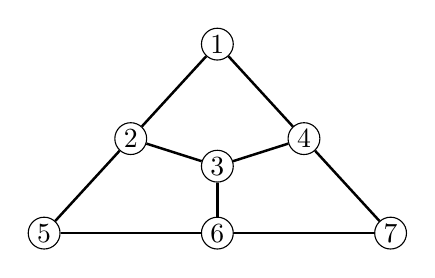
\begin{tikzpicture}[scale=1,
  every node/.style={circle, draw, fill=white, inner sep=1.2pt},
  e/.style={line width=0.9pt}
]

% --- triangle corners ---
\node (1) at (0,2.4) {1};
\node (5) at (-2.2,0) {5};
\node (7) at ( 2.2,0) {7};

% --- place 2,4,6 exactly on the triangle sides ---
% 2 on line segment 5--1, 4 on 1--7, 6 on 5--7
\node (2) at (-1.1,1.2) {2};
\node (4) at ( 1.1,1.2) {4};
\node (6) at (0,0) {6};

% interior node
\node (3) at (0,0.85) {3};

% --- outer triangle boundary as segmented sides ---
\draw[e] (5)--(2)--(1);
\draw[e] (1)--(4)--(7);
\draw[e] (5)--(6)--(7);

% --- interior edges (same as the original structure) ---
\draw[e] (2)--(3)--(4);
\draw[e] (3)--(6);

\end{tikzpicture}
\end{center}
where the stablizer codes are given by looking at the loops of the graph.
\begin{align}
    g_1 &= X_1X_2X_3X_4 \\
    g_2 &= X_2X_3X_5X_6 \\
    g_3 &= X_3X_4X_6X_7  \\
    g_4 & =Z_1Z_2Z_3Z_4 \\
    g_5 &= Z_2Z_3Z_5Z_6 \\
    g_6 &= Z_3Z_4Z_6Z_7  
\end{align}
Is this a valid $S$? Yes, because all the generators commute because there is an even amount of overlapping of $X$'s and $Z$'s. This is because they share edges. \\
$n=7, k=1$ logical qubits. ($n - \text{min \# of generators} = k$) \\
How many possible single-qubit Pauli errors are there? $7\cdot 3 + 1 = 22$ where 1 comes from identity. \\
The number of possible syndrome values is $2^6 = 64$. \\
This is the $[[7,1]]$ \textbf{Steane code}. 
\end{example}

\textit{For a valid stabilizer, $S$ needs to be an Abelian group, and all of its elements commute with each other, and it is sufficient that the generators all commute with each other.}


\begin{example}
    Let $S = \langle XZZXI, IXZZX, XIXZZ, ZXIXZ\rangle$. Then $n=5, k = 1$. This is the $[[5,1]]$ code. There are $5\cdot 3 + 1 = 16$ possible single qubit errors. The number of possible syndrome values is 16, since we have 1 bit for every single generator, and we have 4 bits and $2^4 = 16$. This is called the \textbf{perfect code}, which is the minimum amount of syndromes needed to distinguish all possible single bit errors. 
\end{example}
Quantum Hamming Bound: says that the number of syndrome bits must be at least equal to the number of single qubit errors that happen 
\begin{equation}
    \sum_{j=0}^t 3^j {{n}\choose{k}} \leq 2^{n-k}
\end{equation}
There are other perfect quantum codes: there is a family of these
\begin{equation}
    \left[\left[\frac{4^r -1}{3}, \frac{4^r-1}{3}-2r\right]\right]
\end{equation}
For $r=2, [[5,1]]$ and for $r=3, [[21,15]]$. \\

Stabilizer code properties: 
    \begin{definition}
        weight: for $g \in G$, $wt(g) = \text{\# of non-identity terms in the tensor product expansion}$
    \end{definition}
    \begin{definition}
        distance: 
        \begin{equation}
            d = \min_{E \in G_n, uncorrectible}[w(E)]
        \end{equation}
        s.t. $\braket{\psi_i|E|\psi_j} \neq \delta_{ij} \; \forall \ket{\psi_i} = V_s$, in other words this is the minimum weight of an uncorrectable/undetectable code (smallest error that makes you confused)
    \end{definition}
Weight is about a Pauli string; distance is about a code. \\
We use this distance in the nomenclature $[[n,k,d]]$. \\
For example, the $[[5,1]]$ is actually $[[5,1,3]]$ code since it detects a single qubit error, 3 possible errors. For example: $000,111$ is a [[3,1,3]] code (classical).  \\

\subsection{Classical Linear Codes}
A $[n,k]$ (classical) code is a set of bit strings. \\
Encodes a $k$-bit vector $\Vec{x} \rightarrow F_2^n$ into a $n$-bit vector \\
Recall: $[n,k,d]$ classical code encodes $k$ bits in $n$ bits with distance $d$ \\
Distance $d$ here is Hamming distance $d = \min(d(c_1,c_2)) : c_1, c_2 \in C $
\begin{definition}
    The $n \times k$ generator matrix $G$ encodes data $\vec{x}$ into $\vec{v} = G \vec{x}$ (columns of $G$ are basis codewords)
\end{definition}
\begin{example}
    $G = \begin{pmatrix} 1 \\ 1 \\ 1 \end{pmatrix}$, then $G \begin{pmatrix} 0 \end{pmatrix} = \begin{pmatrix} 0 \\ 0 \\ 0 \end{pmatrix}$ and $G \begin{pmatrix} 1 \end{pmatrix} = \begin{pmatrix} 1 \\ 1 \\ 1 \end{pmatrix}$
\end{example}
\begin{definition}
    The parity check matrix $H$ is an $n - k$ by $n$ matrix s.t. $H\vec{v} = 0 \forall \vec{v} \in C$, $C$ is codespace. Equivalently, $HG=0$ because the columns of $G$ are codewords (defines nullspaces). $H$ is an $(n-k) \times n$ matrix and $G$ is an $n\times k$ matrix. 
\end{definition}
\begin{example}
    From the previous example, $\begin{pmatrix} 0 & 1 & 1 \\ 1 & 1 & 0 \end{pmatrix}$. This checks the parity of the right/left hand bits. The rows of $H$ must be perpendicular to columns of $G$.    
\end{example}
\begin{definition}
    Let $C$ be an $[n.k]$ code with generator $G$, and parity check matrix $H$. Then we define $C^\perp$ is the code with generator $H^T$ and parity check matrix $G^T$. $C^\perp$ is the dual code. 
\end{definition}


\subsection{CSS Codes}
Calderbank, Shor, Steane - CSS Codes is a family of good $[[n,k,d]]$ codes correcting $t$ errors. 
\begin{definition}
    CSS codes (quantum) \textit{We'll be using two classical codes to create one quantum code}\\ 
    Let classical codes $C_1$ be $[n,k_1]$ and $C_2$ be $[n,k_2]$ s.t. $C_2 \subset C_1$, \textit{That is, all the codewords in $C_2$ are also in $C_1$, thus $C_1$ can correct for everything inside $c_2$}, and $c_1$ and $c_2^\perp$ both correct $t$ errors i.e. $H_2 = H(c_2^\perp) = G_2^T$ corrects $t$ errors. Then the code $CSS(C_1,C_2)$ is defined by the following stabilizers which is generated by 
    \begin{equation}
        S = \langle X[H_2], Z[H_1] \rangle 
    \end{equation}
    where $X[\cdot] = \text{replace } 0 \rightarrow I, I\rightarrow X$ and $Z[\cdot] = \text{replace } 0 \rightarrow I, I\rightarrow Z$, and take rows as generators $Rightarrow$ binary notation (binary symplectic matrix representation of a CSS code): 
    \begin{equation}
        \left(\begin{array}{c|c} X & Z \end{array}\right)= \left(\begin{array}{c|c} G_2^{T} & 0\\ \hline 0 & H_2 \end{array}\right)
    \end{equation}
\end{definition} 
$H_2 =$ parity check matrix of $c_2^\perp$ \\ 
$H_1 =$ parity check matrix of $c_1$ \\
$CSS(c_1,c_2)$ has parameters $[[n,k_1-k_2]]$ \\
Is $S$ a valid stabilizer? YES, need elements to commute. This implies that we need $H_2H_1^T = 0$. \\
\begin{equation}
     H_2H_1^T = H(C_2^\perp)H_1^T = G_2^TH_1^T = (H_1G_2)^T = 0
\end{equation}
since $H_1G_1 = 0$ by definition of the parity check matrix and $G_2$ is the set of codewords and $C_2$ is a subspace of the codewords in $G_1$. \\

CSS code idea: $C_1$ corrects bit flips errors ($X$ errors).  This is because $Z[H_1]$ is the parity check matrix for $C_1$ and we made $Z$ stabilizer strings out of it, which anti-commute with $X$ errors. $C_2$ corrects phase flips errors ($Z$ errors). This is because $X[H_2]$ is the parity check matrix for $C_2$ and we made $X$ stabilizer strings out of it, which anti-commute with $Z$ errors. 
\begin{equation}
    CSS(c_1,c_2) = \{\ket{X + c_2} = \frac{1}{\sqrt{\norm{c_2}}} \sum_{y \in c_2} x+y \,|\, \forall x \in C_1\}
\end{equation}


Group picture: $c_2 \subset c_1$, What happens if we add a number to $C_2$? In group theory, if we multiply all the elements of a subgroup by an element of that subgroup, we get a coset. each one of these $\ket{x+c_2}$ is like a coset. $c_1$ corrects bit flips and $c_2$ corrects phase flips. Each coset is a distinct codeword. 

\begin{example}
    $[[7,1,3]]$ is a CSS code. (Here $c_2 = c_1$). \\
    $[[9,1,3]]$ is a CSS code. \\
    $[[5,1,3]]$ is not a CSS code. \\
\end{example}
\section{PSet 2 - 15 February 2025}

\subsection{Problem 1 - Random $Z$-rotations gives phase damping}
Consider a quantum circuit which rotates a single qubit around the $\hat{z}$ axis by a random angle:
\begin{center}
\begin{quantikz}
\lstick{$\rho$}         \qw & \gate{Z(\theta)} & \qw 
\end{quantikz}
\end{center}
where the input qubit is the arbitrary density matrix
\begin{equation}
    \begin{pmatrix} a & b \\ c & d \end{pmatrix}
\end{equation}
and the gate $Z_\theta$ performs the unitary transform 
\begin{equation}
    Z_\theta = e^{-i\theta Z / 2} = \cos\frac{\theta}{2} \mathbb{1} - i \sin \frac{\theta}{2} Z = \begin{pmatrix}\cos\frac{\theta}{2} & 0 \\ 0 & \cos\frac{\theta}{2}\end{pmatrix} - i \begin{pmatrix}\sin\frac{\theta}{2} & 0 \\ 0 & -\sin\frac{\theta}{2}\end{pmatrix} = \begin{pmatrix}\cos\frac{\theta}{2}-i\sin\frac{\theta}{2} & 0 \\ 0 & \cos\frac{\theta}{2} +i \sin\frac{\theta}{2}\end{pmatrix}
\end{equation} 
We can write $Z_\theta$ as 
\begin{equation}
    Z_\theta = e^{-i\theta Z / 2} = \begin{pmatrix}e^{-i\frac{\theta}{2}} & 0 \\ 0 & e^{i\frac{\theta}{2}}\end{pmatrix}
\end{equation} 
and $\theta$ is a random variable with probability distribution
\begin{equation}
    p(\theta) = \frac{1}{2\sqrt{\pi \sigma}} e^{-\theta^2/4\sigma}
\end{equation}
The output of this circuit is 
\begin{equation}
    \mathcal{E}_{PD}(\rho) = \int_{-\infty}^{\infty}Z_\theta \rho Z_\theta^\dagger p(\theta) d\theta
\end{equation}
which maybe understood as being an operator sum representation with an infinite continuously parameterized set of operation elements. \\
We expect the output state $\rho' = \mathcal{E}_{PD}(\rho)$ to look like
\begin{itemize}
    \item The diagonal elements of the input density matrix will stay unchanged
    \item As $\sigma$ increases, the amount of phase damping increases.
\end{itemize}
Let the matrix elements of the output state $\rho' = \mathcal{E}_{PD}(\rho)$ be 
\begin{equation}
    \rho' = \begin{pmatrix}
        \rho_{00}' & \rho_{01}' \\ \rho_{10}' & \rho_{11}'
    \end{pmatrix}
\end{equation}
Then 
\begin{align}
    \mathcal{E}_{PD}(\rho) &= \int_{-\infty}^{\infty} Z_\theta \rho Z_\theta^\dagger p(\theta) d\theta \\
    &= \int_{-\infty}^{\infty} e^{-i\theta Z/2} \rho e^{i\theta Z/2} p(\theta) d\theta \\
    &= \int_{-\infty}^{\infty} \begin{pmatrix}e^{-i\frac{\theta}{2}} & 0 \\ 0 & e^{i\frac{\theta}{2}}\end{pmatrix}   \begin{pmatrix} a & b \\ c & d \end{pmatrix} \begin{pmatrix}e^{i\frac{\theta}{2}} & 0 \\ 0 & e^{-i\frac{\theta}{2}}\end{pmatrix} p(\theta) d\theta \\
    &=  \int_{-\infty}^{\infty} \begin{pmatrix} ae^{-i\frac{\theta}{2}} & be^{-i\frac{\theta}{2}} \\ ce^{i\frac{\theta}{2}} & de^{i\frac{\theta}{2}} \end{pmatrix} \begin{pmatrix}e^{i\frac{\theta}{2}} & 0 \\ 0 & e^{-i\frac{\theta}{2}}\end{pmatrix} p(\theta) d\theta \\
    &= \int_{-\infty}^{\infty} \begin{pmatrix} a & b e^{-i \theta} \\ ce^{i \theta} & d \end{pmatrix}  p(\theta) d\theta \\
    &= \frac{1}{2\sqrt{\pi \omega}} \int_{-\infty}^{\infty} \begin{pmatrix} a & b e^{-i \theta} \\ ce^{i \theta} & d \end{pmatrix}  e^{-\theta^2/4\sigma} d\theta \\
\end{align}
For the diagonal term, 
\begin{align}
    \rho_{00}' = \frac{a }{2\sqrt{\pi \sigma}} \int_{-\infty}^{\infty} a e^{-\theta^2/4\sigma} = \frac{a}{2\sqrt{\pi \sigma}} \sqrt{4 \pi \sigma } = a 
\end{align}
For the off-diagonal term, using completing the square: 
\begin{align}
    (\theta + A)^2 = \theta ^2 + 2 A \theta + A^2
\end{align}
In this case, $A = 2 i \sigma$, therefore, 
\begin{align}
    (\theta + 2i\sigma)^2 &= \theta ^2 + 2 ( 2 i \sigma) \theta + ( 2 i \sigma)^2 \\
    &= \theta^2 + 4 i \sigma \theta - 4\sigma^2
\end{align}
Therefore, 
\begin{align}
    \rho_{01}'  = \frac{b }{2\sqrt{\pi \sigma}} \int_{-\infty}^{\infty} b e^{-\frac{\theta^2}{4\sigma} - i \theta} =  \frac{b }{2\sqrt{\pi \sigma}} \int_{-\infty}^{\infty} b e^{\frac{-(\theta^2 + 4i\sigma\theta) }
    {4\sigma}} = \int_{-\infty}^{\infty} b e^{ -\frac{(\theta -2 i\sigma)^2}{4\sigma} e^ {-\sigma}}  = \frac{b}{2\sqrt{\pi \sigma}} \sqrt{4\pi\sigma}e^{-\sigma} = b e^{-\sigma}  
\end{align}
Therefore, the matrix $\rho' = \mathcal{E}_{PD}(\rho)$ is given by
\begin{equation}
    \rho' = \begin{pmatrix} a & b e^{-\sigma} \\ ce^{-\sigma} & d \end{pmatrix} \\
\end{equation}



\newpage
\subsection{Problem 2 - Phase damping and T2 decay}
How is phase damping observed experimentally, as a physical process? Since phase damping causes loss of coherence, i.e. phase information in superposition states, it is natural to observe and quantify phase damping by creating a superposition state, letting phase damping occur, then un-creating the superposition. Such a sequence of steps is precisely the interferometer studied in the last problem set, now with phase damping between the two Hadamard gates:
\begin{center}
\begin{quantikz}
\lstick{$\ket{\psi}$}         \qw & \gate{H} & \gate{\mathcal{E}_{PD}} & \gate{H} & \qw 
\end{quantikz}
\end{center}
Let the input state be $\ket{\psi} = \ket{0}$, and let $\mathcal{E}_{PD}$ be the phase damping via random $\hat{z}$ rotations you just worked out above. The output density matrix $\rho''$ of this quantum interferometer circuit is:
\begin{equation}
    \rho' = H \mathcal{E}_{PD}(H\ketbra{\psi}H)H
\end{equation}
We expect the output state $\rho' = \mathcal{E}_{PD}(\rho)$ to look like
\begin{itemize}
    \item When $\sigma=0$, there will be no phase damping, and the output state will be $\ket{0}$
    \item As $\sigma \rightarrow \infty$ the output $\rho' \rightarrow \ketbra{1}$.
\end{itemize}
We are given that $\ket{\psi} = 0$, therefore,
\begin{equation}
    \ketbra{\psi} = \begin{pmatrix}1 & 0 \\ 0 & 0\end{pmatrix}
\end{equation}
Calculating $H\ketbra{\psi}H$,
\begin{align}
    H\ketbra{\psi}H &= \frac{1}{2}\begin{pmatrix}1 & 1 \\ 1 & -1\end{pmatrix} \begin{pmatrix}1 & 0 \\ 0 & 0\end{pmatrix} \begin{pmatrix}1 & 1 \\ 1 & -1\end{pmatrix} \\
    &= \frac{1}{2}\begin{pmatrix}1 & 0 \\ 1 & 0\end{pmatrix} \begin{pmatrix}1 & 1 \\ 1 & -1\end{pmatrix} \\
    H\ketbra{\psi}H &= \frac{1}{2} \begin{pmatrix}1 & 1 \\ 1 & 1\end{pmatrix}
\end{align}
From the previous problem we have that 
\begin{equation}
    \rho' = \begin{pmatrix} a & b e^{-\sigma} \\ ce^{-\sigma} & d \end{pmatrix} \\
\end{equation}
Therefore, 
\begin{equation}
    \mathcal{E}(H\ketbra{\psi}H) = \frac{1}{2}\begin{pmatrix} 1 & e^{-\sigma} \\ e^{-\sigma} & 1 \end{pmatrix}
\end{equation}
Then,
\begin{align}
    H \mathcal{E}(H\ketbra{\psi}H) H &= \frac{1}{4} \begin{pmatrix}1 & 1 \\ 1 & -1\end{pmatrix} \begin{pmatrix} 1 & e^{-\sigma} \\ e^{-\sigma} & 1 \end{pmatrix} \begin{pmatrix}1 & 1 \\ 1 & -1\end{pmatrix} \\
    &= \frac{1}{4} \begin{pmatrix}1+e^{-\sigma} & 1+e^{-\sigma} \\ 1-e^{-\sigma} & -1+e^{-\sigma}\end{pmatrix} \begin{pmatrix}1 & 1 \\ 1 & -1\end{pmatrix} \\
    &= \frac{1}{4} \begin{pmatrix}2+2e^{-\sigma} & 0 \\ 0 & 2-2e^{-\sigma}\end{pmatrix} \\
    &= \frac{1}{2} \begin{pmatrix}1+e^{-\sigma} & 0 \\ 0 & 1-e^{-\sigma}\end{pmatrix}
\end{align}


\newpage
\subsection{Problem 3 - Spin echo and T2}
Real physical systems often have behavior that is correlated in time. Specifically, for example, phase damping at two times may have rotation angles which are correlated with each other, instead of being independent. Such correlations mean that there is less inherent randomness than if the damping were independent processes. \\

Consider a scenario similar to before, where a single qubit interferometer is used to quantify phase coherence, but this time, let there be two random rotations applied, with angles $\theta_1$ and $\theta_2$. \\

Each of these angles has a gaussian distribution with zero mean and variance $\sigma$, but now let them be correlated, such that the joint probability distribution for $\theta_1$ and $\theta_2$ is
\begin{equation}
    p(\theta_1, \theta_2) = \frac{1}{2\pi \sigma \sqrt{1-r^2}} \exp\left[-\frac{1}{2(1-r^2)\sigma} (\theta_1^2 + \theta_2^2 - 2r\theta_1\theta_2)\right]
\end{equation}
Here, $r$ parameterizes the strength of the correlation; when $r=0$, the two angles are uncorrelated with each other. And as $r \rightarrow 1$, they approach being perfectly correlated. Confirm for yourself that $p(\theta_1,\theta_2)$ is a proper probability distribution. \\

When the phase rotation noise is correlated, its effects can be (partially) reversed by adding a spin echo pulse in middle of the noise process. This spin-echo pulse is just an $X$ gate. Because $X$ flips the $\ket{0}$ and $\ket{1}$ states of the qubit, it also reverses correlated rotations. Mathematically, this is because $XZX = -Z$.\\

We can quantify this effect by analyzing this quantum interferometer circuit with spin echo pulses:
\begin{center}
    \begin{quantikz}
        \lstick{$\ket{\psi}$} & \gate{H} & \gate{Z_{\theta_1}} & \gate{X} & \gate{Z_{\theta_2}} & \gate{X} & \gate{H} & 
    \end{quantikz}
\end{center}

Note that we have included two $X$ gates to mathematically simplify the analysis; the second $X$ gate could be left out to give a simpler but fully equivalently effective circuit. \\

Let the input qubit state be $\ket{\psi} = \ket{0}$, and let $\mathcal{E}_1$ and $\mathcal{E}_2$ be the channels obtained by averaging over $Z_{\theta_1}$ and $Z_{\theta_2}$, respectively, such that the final output state is then 
\begin{align}
    \rho' &= H X \mathcal{E}_2(X\mathcal{E}_1(H\ketbra{\psi}H X)X) XH \\
    &= \int_{-\infty}^{\infty} \int_{-\infty}^{\infty}HXe^{i}
\end{align}




\newpage
\subsection{Problem 4 - Getting started with stim}
We want to write code that will define a procedure which returns True if the two provided PauliString objects commute, and False otherwise. 
\begin{lstlisting}
    def ps_commute(a:stim.PauliString, b:stim.PauliString) -> bool:
    
        # Write code using stim which reutrns True
        # if a commutes with b, and False otherwise
        return a.commutes(b)
\end{lstlisting}



\newpage
\subsection{Problem 5 - Groups and generators}
Recall that an $n$-qubit state $\ket{\psi}$ is stabilized by an operator $g$ if $g\ket{\psi} = \ket{\psi}$. \\
We define a stabilizer
\begin{equation}
    \mathcal{S} = \{g \in G_n\,:\, g\ket{\psi} = \ket{\psi}\}
\end{equation}
where $G_n$ is the $n$-qubit Pauli group.\\

Note that $\mathcal{S}$ is a group:
\begin{itemize}
    \item $I^{\otimes n} \ket{\psi} = \ket{\psi}$ is the identity element
    \item $g$ has an inverse in $S$: namely $g^{-1} = g^{\dagger} = g$ 
    \item Multiplication is associative
    \item The set $\mathcal{S}$ is closed under multiplication: $(gg')\ket{\psi} = g\ket{\psi} = \ket{\psi}$
\end{itemize}
You can verify that if $\mathcal{S}$ stabilizes a non-trivial vector space, it must further hold that all elements of the stabilizer must commute with each other (so that states that share simultaneous eigenspaces) and that $-I \notin \mathcal{S}$. \\

Stabilizers are one of the nose useful ways to describe states and transformations in quantum information. In this problem, we explore some basic properties of stabilizer sets which arise from the fact that a stabilizer is an Abelian group (commutative group). \\

You are given that 
\begin{equation}
    \mathcal{S} = \{XXIZ, YXIY,IZIX,ZZII,-YYIZ,XYIY,ZIIX,IIII\}
\end{equation}
Give the shortest possible elements which can be combined by multiplication to produce all of the elements in $S$. We say such a list is a set of \textit{generators} of $\mathcal{S}$. \\

We are given that $\dim{S} = 8$, therefore, the minimum amount of generators is $8=2^m \rightarrow m=3$ independent generators. Let 
\begin{equation}
    S = \langle ZZII, IZIX, XXIZ\rangle
\end{equation}
where
\begin{align}
    g_1 &= ZZII \\
    g_2 &= IZIX \\
    g_3 &= XXIZ 
\end{align}
Then,
\begin{align}
    I &\in S \\
    g_1g_2 &= (ZZII)(IZIX) = ZIIX \in S\\
    g_1g_3 &= (ZZII)(XXIZ) = (-i*-i)(YYIZ) = -YYIZ \in S \\ 
    g_2g_3 &= (IZIX)(XXIZ) = (-i*i)(XYIY) = XYIY \in S \\ 
    g_1g_2g_3 &= (ZZII)(IZIX)(XXIZ) = (ZIIX)(XXIZ) = (i*-i)(YXIY) = YXIY
\end{align}
Therefore, 
\begin{equation}
    S = \langle ZZII, IZIX, XXIZ\rangle
\end{equation}



\newpage
\subsection{Problem 6 - Groups and generators II}
Given that $\{XIX,ZIY\}$ generate $\mathcal{S}$. Give a list of additional operators which are also in $\mathcal{S}$. \\
Using 
\begin{equation}
    XZ = -iY \text{ and } XY = iZ
\end{equation}
Then we have, 
\begin{equation}
    (XIX)(ZIY) = (-i^2)YIZ = YIZ
\end{equation}
We also need identity, therefore, the additional operators are $\{III,YIZ\}$



\newpage
\subsection{Problem 7 - Elementary stabilizers}
Stabilizers are one of the most useful ways to describe states and transformations in quantum information. In this problem, we explore some descriptions of basic stabilizer states. \\

Recall that if an $n$-qubit state $\ket{\psi}$ is stabilized by $S = \langle g_1, g_2, \ldots, g_n\rangle$, then $g\ket{\psi} = \ket{\psi}$ for all $g \in \mathcal{S}$. Note that $g_1, g_2, \ldots, g_n$ are the \textit{generators} of $\mathcal{S}$. \\

We will give stabilizer generator sets for the following states (normalizations suppressed). 
We will use the following
\begin{align}
    Z\ket{0} &= \ket{0}\\
    Z\ket{1} &= -\ket{1}\\
    X\ket{0} &= \ket{1}\\
    X\ket{1} &= \ket{0}
\end{align}

\begin{itemize}
    \item $\ket{0} + i\ket{1} \Rightarrow \boxed{S = \langle Y\rangle}$ 
    \item $\ket{1} \Rightarrow \boxed{S = \langle -Z \rangle}$
    \item $\ket{00} + \ket{11} \Rightarrow \boxed{S = \langle ZZ, XX\rangle}$
    \item $\ket{00} - \ket{11} \Rightarrow \boxed{S = \langle ZZ, -XX\rangle}$
    \item $\ket{000} + \ket{111} \Rightarrow \boxed{S = \langle XXX, ZZI, IZZ\rangle}$
\end{itemize}



\newpage
\subsection{Problem 8 - Elementary stabilizers II}
Given stabilizer generator sets for the following \textit{vector spaces}, specified by the basis sets given.
\begin{align}
    Z\ket{0} &= \ket{0}\\
    Z\ket{1} &= -\ket{1}\\
    X\ket{0} &= \ket{1}\\
    X\ket{1} &= \ket{0}
\end{align}
\begin{itemize}
    \item $\{\ket{001}, \ket{110}\} \Rightarrow \boxed{S = \langle ZZI, -ZIZ\rangle}$ \\
    \textit{Check:}
    \begin{align}
        ZZI\ket{001} &= \ket{001} \\ 
        -ZIZ\ket{001} &= \ket{001} \\ 
        ZZI\ket{110} &= \ket{110}  \\
        -ZIZ\ket{110} &= \ket{110}
    \end{align}
    \item $\{\ket{00} + \ket{11}, \ket{01} + \ket{10}\} \Rightarrow \boxed{S = \langle XX\rangle}$ \\
    \textit{Check:}
    \begin{align}
        XX(\ket{00} + \ket{11}) &= \ket{11} + \ket{00}  = \ket{00} + \ket{11}\\ 
        XX(\ket{01} + \ket{10}) &= \ket{10} + \ket{01}  = \ket{01} + \ket{10}
    \end{align}
    
\end{itemize}



\newpage
\subsection{Problem 9 - Action of quantum gates on stabilizer states}
Suppose $\ket{\psi}$ is stabilized by $\mathcal{S}$ such that $g\ket{\psi} = \ket{\psi}$ for all $g \in \mathcal{S}$. Then $\ket{\phi} = U\ket{\phi}$ is stabilized by $S' = USU^\dagger$, since
\begin{equation}
    UgU^\dagger \ket{\phi} = UgU^\dagger U \ket{\psi} = U \ket{\psi} = \ket{\phi}
\end{equation}
Thus we may often gain deep appreciation into the operation of a quantum circuit $U$ by studying how it transforms stabilizer sets (by conjugation), rather than how it transforms general quantum states (by multiplication). \\

Consider the vector space $V = \{\ket{01} + \ket{10}, \ket{00} + \ket{11}\}$ stabilized by the generator set $\mathcal{S} = \langle XX \rangle$. We want to find the new stabilizer $S'$ resulting from operating on this two qubit vector space with the following unitary gates. 
\begin{itemize}
    \item $U = H^{\otimes 2} = H \otimes H$ 
    \begin{align}
        S' &= \langle(H \otimes H)(X \otimes X)(H^\dagger \otimes H^\dagger)\rangle \\
        &= \langle (HXH)\otimes (HXH)\rangle \\
        \Aboxed{S' &= \langle ZZ\rangle}
    \end{align}
    
    \item $U = S^{\otimes 2} = S \otimes S$ 
    \begin{align}
        S' &= \langle(S \otimes S)(X \otimes X)(S^\dagger \otimes S^\dagger)\rangle \\
        &= \langle (SXS^\dagger)\otimes (SXS^\dagger)\rangle \\
        \Aboxed{S' &= \langle ZZ\rangle}
    \end{align}
    
    \item $U = T^{\otimes 2} = T\otimes T$ 
    \begin{align}
        TXT^\dagger &= \begin{pmatrix} 1 & 0 \\ 0 & e^{i\pi/4} \end{pmatrix} \begin{pmatrix} 0 & 1 \\ 1 & 0 \end{pmatrix} \begin{pmatrix} 1 & 0 \\ 0 & e^{-i\pi/4} \end{pmatrix} = \begin{pmatrix} 0 & 1 \\ e^{i\pi/4} & 0 \end{pmatrix}\begin{pmatrix} 1 & 0 \\ 0 & e^{-i\pi/4} \end{pmatrix} = \begin{pmatrix} 0 & e^{-i\pi/4} \\ e^{i\pi/4} & 0 \end{pmatrix} = \frac{1}{\sqrt{2}} \begin{pmatrix} 0 & 1-i \\ 1+i & 0 \end{pmatrix} \\
        &= \frac{1}{\sqrt{2}}(X + Y)
    \end{align}
    Therefore, 
    \begin{align}
        S' &= \langle(T \otimes T)(X \otimes X)(T^\dagger \otimes T^\dagger)\rangle \\
        &= \langle (TXT^\dagger)\otimes (TXT^\dagger)\rangle \\
        &= \left\langle \left(\frac{1}{\sqrt{2}}(X + Y))\otimes (\frac{1}{\sqrt{2}}(X + Y)\right)\right\rangle \\
        \Aboxed{S' &= \emptyset}
    \end{align}
    \item $U = Z^{\otimes 2} = Z\otimes Z$ 
    \begin{align}
        S' &= \langle(Z \otimes Z^\dagger)(X \otimes X)(Z^\dagger \otimes Z^\dagger)\rangle \\
        &= \langle (ZXZ)\otimes (ZXZ)\rangle \\
        \Aboxed{S' &= \langle XX\rangle}
    \end{align}
  
    \item $U = CNOT = ((I+Z) \otimes I + (I-Z)\otimes X) / 2$ \\
    Rewriting $CNOT$ by evaluating $I\pm Z$
    \begin{equation}
        \frac{I+Z}{2} = \ketbra{0} \qquad \frac{I-Z}{2} = \ketbra{1}
    \end{equation}
    Therefore CNOT can be written as 
    \begin{equation}
        U = \ketbra{0}\otimes I + \ketbra{1} \otimes X
    \end{equation}
    Then,
    \begin{align}
        CNOT\,(X \otimes X) \,CNOT &= (\ketbra{0}\otimes I + \ketbra{1} \otimes X)(X \otimes X)(\ketbra{0}\otimes I + \ketbra{1} \otimes X) \\
        &= (\ketbra{0}\otimes I)(X \otimes X)(\ketbra{0}\otimes I) \notag \\
        &\qquad + (\ketbra{0}\otimes I)(X \otimes X)(\ketbra{1}\otimes X) \notag \\
        &\qquad + (\ketbra{1}\otimes X)(X \otimes X)(\ketbra{0}\otimes I) \notag \\
        &\qquad + (\ketbra{1}\otimes X)(X \otimes X)(\ketbra{1}\otimes X) \\
        &= \cancel{(\ketbra{0}\!X\!\ketbra{0})} \otimes (IXI) + (\ketbra{0}\!X\!\ketbra{1}) \otimes (IXX) \notag \\
        &\qquad + (\ketbra{1}\!X\!\ketbra{0}) \otimes (XXI) + \cancel{(\ketbra{1}\!X\!\ketbra{1})} \otimes (XXX) \\
        &=(\ketbra{0}{1}\otimes I) + (\ketbra{1}{0} \otimes I) \\
        &=X \otimes I
    \end{align}
    Therefore, 
    \begin{equation}
        S' = \langle X \otimes I \rangle
    \end{equation}
\end{itemize}



\newpage
\subsection{Problem 10 - Action of quantum gates on stabilizer states II}
Consider the vector space $V$ stabilized by $\mathcal{S} = \langle g_1, g_2, g_3 \rangle$ where
\begin{align}
    g_1 &= IIZZ \\
    g_2 &= ZZII \\
    g_2 &= XXXX
\end{align}
Give the new stabilizer $S'$ resulting from operating on this two qubit vector space with the following unitary gates

\begin{itemize}
    \item $U_1 = H^{\otimes 4}$ 
    \begin{align}
        U_1g_1U_1^\dagger &= (HHHH)(IIZZ)(HHHH) \\
        &= (HIH)(HIH)(HZH)(HZH) \\
        U_1g_1U_1^\dagger & = IIXX \\
        &\notag \\
        U_1g_2U_1^\dagger &= (HHHH)(ZZII)(HHHH) \\
        &= (HZH)(HZH)(HIH)(HIH) \\
        U_1g_2U_1^\dagger & = XXII \\
        &\notag \\
        U_1g_3U_1^\dagger &= (HHHH)(XXXX)(HHHH) \\
        &= (HXH)(HXH)(HXH)(HXH) \\
        U_1g_2U_1^\dagger & = ZZZZ 
    \end{align}
    Therefore,
    \begin{equation}
        \boxed{S' = \langle IIXX, XXII,ZZZZ \rangle}
    \end{equation}
    
    \item $U_2 = S^{\otimes 4}$
    \begin{align}
        U_2g_1U_2^\dagger &= (SSSS)(IIZZ)(S^\dagger S^\dagger S^\dagger S^\dagger ) \\
        &= (SIS^\dagger)(SIS^\dagger)(SZS^\dagger)(SZS^\dagger) \\
        U_2g_1U_2^\dagger & = IIZZ \\
        &\notag \\
        U_2g_2U_2^\dagger &= (HHHH)(ZZII)(S^\dagger S^\dagger S^\dagger S^\dagger) \\
        &= (SZS^\dagger)(SZS^\dagger)(SIS^\dagger)(SIS^\dagger) \\
        U_2g_2U_2^\dagger & = ZZII \\
        &\notag \\
        U_2g_3U_2^\dagger &= (HHHH)(XXXX)(S^\dagger S^\dagger S^\dagger S^\dagger) \\
        &= (SXS^\dagger)(SXS^\dagger)(SXS^\dagger)(SXS^\dagger) \\
        U_1g_2U_1^\dagger & = YYYY 
    \end{align}
    Therefore,
    \begin{equation}
        \boxed{S' = \langle IIZZ, ZZII, YYYY \rangle}
    \end{equation}
    
    \item $U_3 = Z^{\otimes 4}$
    \begin{align}
        U_3g_1U_3^\dagger &= (ZZZZ)(IIZZ)(ZZZZ) \\
        &= (ZIZ)(ZIZ)(ZZZ)(ZZZ) \\
        U_3g_1U_3^\dagger & = IIZZ \\
        &\notag \\
        U_3g_2U_3^\dagger &= (ZZZZ)(ZZII)(ZZZZ) \\
        &= (ZZZ)(ZZZ)(ZIZ)(ZIZ) \\
        U_3g_2U_3^\dagger & = ZZII \\
        &\notag \\
        U_3g_3U_3^\dagger &= (ZZZZ)(XXXX)(ZZZZ) \\
        &= (ZXZ)(ZXZ)(ZXZ)(ZXZ) \\
        U_3g_2U_3^\dagger & = XXXX 
    \end{align}
    Therefore,
    \begin{equation}
        \boxed{S' = \langle IIZZ, ZZII, XXXX \rangle}
    \end{equation}
\end{itemize}



\newpage
\subsection{Problem 11 - Action of quantum gates on stabilizer states III}
Two stabilizer sets $\mathcal{S}$ and $\mathcal{S}'$ are equal if they contain the same stabilizer elements, i.e. if their generators generate the same sets. For the definitions of $U_1$, $U_2$, and $U_3$ and $\mathcal{S} = \langle g_1, g_2, g_3 \rangle$, are $\mathcal{S}$ and $\mathcal{S}?$ the same? \\
From problem 10:
\begin{align}
    S &= \langle IIZZ, ZZII, XXXX \rangle \\
    S_1' & = \langle IIXX, XXII,ZZZZ \rangle \\
    S_2' & = \langle IIZZ, ZZII, YYYY \rangle \\
    S_3' & =  \langle IIZZ, ZZII, XXXX \rangle
\end{align}

\begin{itemize}
    \item $U_1SU_1^\dagger = S$? False, because 
    \item $U_2SU_2^\dagger = S$? True, because the first two elements are in $S$. Then: 
    \begin{equation}
        (IIZZ)(ZZII)(YYYY) = (ZZZZ)(YYYY) = (-i)^4XXXX = XXXX
    \end{equation}
    \item $U_3SU_3^\dagger = S$? True, because the generators are exactly the same
\end{itemize}



\newpage
\subsection{Problem 12 - Stabilizer description of quantum circuit transformations}
Consider the following simple quantum circuit:
\begin{center}
    \begin{quantikz}
        &\slice{$S_0$} & \gate{H} \slice{$S_1$} & \ctrl{1} \slice{$S_2$} & & \\
        & & & \targ{} & &
    \end{quantikz}
\end{center}
The input state is $\ket{00}$, which is stabilized by $S_0 = \langle IZ, ZI \rangle$. Give the stabilizers describing the state after the Hadamard and after the controlled-NOT gate (the top wire carries the first qubit). \\

We can work this out by using the fact that $U$ acting on a state stabilized by $\mathcal{S}$ produces a state stabilized by $USU^\dagger$. \\

You can also double-check yourself by working out the explicit quantum states produced in the circuit, and figuring out the stabilizers for each of the states. However, for circuits composed of Clifford group gates, namely circuits generated by $H$, $S$, and the controlled-NOT gate, it is much faster to work directly with the stabilizer. 


\newpage
\subsection{Problem 13 - 7-bit Hamming code syndrome and distance}
Consider the classical $n=7$, $k=4$ code $C$ generated by
\begin{equation}
G=
\begin{pmatrix}
1 & 0 & 0 & 0\\
0 & 1 & 0 & 0\\
0 & 0 & 1 & 0\\
0 & 0 & 0 & 1\\
0 & 1 & 1 & 1\\
1 & 0 & 1 & 1\\
1 & 1 & 0 & 1
\end{pmatrix}
\end{equation}
which encodes sixteen seven-bit codewords. Let us use as the parity check matrix
\begin{equation}
H=
\begin{pmatrix}
0 & 0 & 0 & 1 & 1 & 1 & 1\\
0 & 1 & 1 & 0 & 0 & 1 & 1\\
1 & 0 & 1 & 0 & 1 & 0 & 1
\end{pmatrix}
\end{equation}

Recall that for these binary matrices, addition is performed modulo two, and note that $HG=0$.

\begin{enumerate}
\item An error can be modeled as addition (modulo 2) of a random bit string $e$ to a codeword
$x\in C$, giving $y=x+e$. As long as $y$ is not a codeword, the error can be detected by computing
\begin{equation}
Hy = He \neq 0.
\end{equation}
Thus, $Hy$ is called the \emph{error syndrome}.

Give the error syndrome for the following bit strings. 
\begin{itemize}
    \item $y_0^{T} = \begin{pmatrix}0 & 1 & 1 & 1 & 1 & 0 & 0 \end{pmatrix}$: 
    \begin{align}
        H y_0^T &= \begin{pmatrix}
        0 & 0 & 0 & 1 & 1 & 1 & 1\\
        0 & 1 & 1 & 0 & 0 & 1 & 1\\
        1 & 0 & 1 & 0 & 1 & 0 & 1\end{pmatrix} \begin{pmatrix}0 \\ 1 \\ 1 \\ 1 \\ 1 \\ 0 \\ 0 \end{pmatrix} \\
        H y_0^T &= \begin{pmatrix} 0 & 0 & 0 \end{pmatrix}^T
    \end{align}

    \item $y_1^T = \begin{pmatrix} 1 & 1 & 1 & 1 & 1 & 0 & 0 \end{pmatrix}$:
    \begin{align}
        H y_0^T &= \begin{pmatrix}
        0 & 0 & 0 & 1 & 1 & 1 & 1\\
        0 & 1 & 1 & 0 & 0 & 1 & 1\\
        1 & 0 & 1 & 0 & 1 & 0 & 1\end{pmatrix} \begin{pmatrix} 1 \\ 1 \\ 1 \\ 1 \\ 1 \\ 0 \\ 0\end{pmatrix} \\
        H y_1^T &= \begin{pmatrix} 0 & 0 & 1 \end{pmatrix}^T
    \end{align}

    \item $y_1^T = \begin{pmatrix} 0 & 1 & 0 & 1 & 1 & 0 & 0 \end{pmatrix}$
    \begin{align}
        H y_0^T &= \begin{pmatrix}
        0 & 0 & 0 & 1 & 1 & 1 & 1\\
        0 & 1 & 1 & 0 & 0 & 1 & 1\\
        1 & 0 & 1 & 0 & 1 & 0 & 1\end{pmatrix} \begin{pmatrix} 0 \\ 1 \\ 0 \\ 1 \\ 1 \\ 0 \\ 0\end{pmatrix} \\
        H y_2^T &= \begin{pmatrix} 0 & 1 & 1 \end{pmatrix}^T
    \end{align}
\end{itemize}

\item The maximum number of bit flip errors that can be tolerated is determined by the minimum Hamming distance between any two codewords, 
\begin{equation}
    d(C) = \min_{x,y \in C, x \neq y} d(x,y)
\end{equation}
where $d(x,y)$ is the number of bits where $x$ and $y$ differ. We want to calculate $d(C)$ for the above code.\\
We know that if code has distance $d$, then $H$ has at least $d$ linearly independent columns. We don't have $d(c) = 1$ because no matter where you put a $1$ in the $y^T$, the result will never be 0. We also don't have $d(c) = 2$ for the same reason, there will always be a $1$ when calculating $H_y^T$. Let $y^T = \begin{pmatrix}1 & 1 & 1 & 0 & 0 & 0 & 0\end{pmatrix}^T$. Then $Hy^T=0$. 

\begin{center}
$d(C)=3$ for the above code 
\end{center}
\end{enumerate}



\newpage
\subsection{Problem 14 - Dual classical code}
onsider the classical $n=7$, $k=4$ code $C$ generated by
\begin{equation}
G=
\begin{pmatrix}
1 & 0 & 0 & 0\\
0 & 1 & 0 & 0\\
0 & 0 & 1 & 0\\
0 & 0 & 0 & 1\\
0 & 1 & 1 & 1\\
1 & 0 & 1 & 1\\
1 & 1 & 0 & 1
\end{pmatrix}
\end{equation}
which encodes sixteen seven-bit codewords. Let us use as the parity check matrix
\begin{equation}
H=
\begin{pmatrix}
0 & 0 & 0 & 1 & 1 & 1 & 1\\
0 & 1 & 1 & 0 & 0 & 1 & 1\\
1 & 0 & 1 & 0 & 1 & 0 & 1
\end{pmatrix}
\end{equation}

Recall that for these binary matrices, addition is performed modulo two, and note that $HG=0$.\\

Define a new code $C^\perp$ which has generator matrix $G' = H^T$ and parity check matrix $H'= G^T$. This code is known as the dual of $C$. Recall that $n$ is the number of bits each codeword has, and $k$ is the number of bits which can be encoded by the codewords, i.e. $k = \log_2(\text{number of codewords}) $. \\

Here,
\begin{equation}
    G' = H^T = \begin{pmatrix}
        0 & 0 & 1 \\ 
        0 & 1 & 0 \\
        0 & 1 & 1 \\ 
        1 & 0 & 0 \\
        1 & 0 & 1 \\
        1 & 1 & 0 \\
        1 & 1 & 1 
    \end{pmatrix}
\end{equation}
and 
\begin{equation}
    H' = G^T = \begin{pmatrix}
        1 & 0 & 0 & 0 & 0 & 1 & 1 \\
        0 & 1 & 0 & 0 & 1 & 0 & 0 \\
        0 & 0 & 1 & 0 & 1 & 1 & 0 \\
        0 & 0 & 0 & 1 & 1 & 1 & 1
    \end{pmatrix}
\end{equation}

\begin{itemize}
    \item A code's $n$ is the length of each codeword. The dual code $C^\perp$ has generator matrix $G' = H^T$, which has dimensions $7 \times 3$. A generator matrix with 7 rows produces codewords with 7 bits. 
        
    Therefore, for $C^\perp$, $n = 7$. 
    \item $k$ is the number of information bits, i.e. the dimension of the code, which equals the rank of the generator matrix. The rank of $G'=H^T = 3$ therefore, $k=3$. 
    \item We want to know if all code words of $C^\perp$ codewords of $C$. The codewords of $C$ are given by 
    \begin{align}
        h_1 &= \begin{pmatrix}0 & 0 & 0 & 1 & 1 & 1 & 1 \end{pmatrix}^T\\
        h_2 &= \begin{pmatrix}0 & 1 & 1 & 0 & 0 & 1 & 1 \end{pmatrix}^T \\
        h_3 &= \begin{pmatrix}1 & 0 & 1 & 0 & 1 & 0 & 1 \end{pmatrix}^T 
    \end{align}
    The codewords of $C^\perp$ are given by
    \begin{align}
        g_1 &= \begin{pmatrix}1 & 0 & 0 & 0 & 0 & 1 & 1 \end{pmatrix}^T\\
        g_2 &= \begin{pmatrix}0 & 1 & 0 & 0 & 1 & 0 & 1 \end{pmatrix}^T \\
        g_3 &= \begin{pmatrix}0 & 0 & 1 & 0 & 1 & 1 & 0 \end{pmatrix}^T \\
        g_4 &= \begin{pmatrix}0 & 0 & 0 & 1 & 1 & 0 & 1 \end{pmatrix}^T 
    \end{align}
    We can see that $h_1 = g_4 = G(0,0,0,1)^T$, $h_2 = g_2 + g_3 = G(0,1,1,0)^T$, and $h_3 = g_1 + g_3 = G(1,0,1,0)^T$. Therefore, all codewords of $C^\perp$ codewords of $C$.
    
\end{itemize}
%%%%% Week 3 %%%%% 
\section{Lecture 5: Graph and Surface Codes - 17 February 2026}
Lecture Outline:
\begin{enumerate}[label=(\Roman*)]
    \item Graph States
    \item Graph Codes
    \item Surface Codes
\end{enumerate}

Last time: $S = \langle g_1, g_2, \cdots, g_{n-k} \rangle \rightarrow c(s)$ corrects $\{E_a\}$ if $\exists g \in S$ s.t. $Eg=-gE$, $\forall E = E_a^\dagger E_b$. If we have an element of the generator that anti-commutes with $E$, then we can detect it because it gives us a syndrome bit and that anti-commutation is the signature of an error having happened. 


\subsection{Graph States}
Goal: systematic construction of stabilizer codes\\
\textit{Codes have more than one state}
\begin{definition}
    A graph state (for graph $G$) is a stabilizer state with generator matrix in the symplectic representation
    \begin{equation}
        \left(\begin{array}{c|c} I & A \end{array}\right)
    \end{equation}
    Where $I$ (identity matrix) are the $X$ stabilizers and $A$ (adjacency) are the $Z$ stabilizers. $X$'s on vertices, and $Z$'s on edges.
\end{definition}
\begin{example}
    \begin{equation}
        \ket{\,%
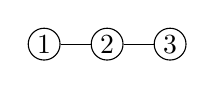
\begin{tikzpicture}[baseline=-0.6ex]
  \node[circle,draw,inner sep=1.2pt] (v1) at (0,0) {$1$};
  \node[circle,draw,inner sep=1.2pt] (v2) at (0.8,0) {$2$};
  \node[circle,draw,inner sep=1.2pt] (v3) at (1.6,0) {$3$};
  \draw (v1) -- (v2) -- (v3);
\end{tikzpicture}
\,} = \begin{pmatrix}
         X & Z & I \\
         Z & X & Z \\ 
         I & Z & X
     \end{pmatrix}
    \end{equation}
     Let $g_1 = XZI$, $g_2 = ZXZ$, $g_3=IZX$, this is a valid generator because there is an even amount of collisions of $X$'s and $Z$'s. 
\end{example}
\begin{example}
    \begin{equation}
        \Bigg|\,%
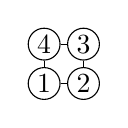
\begin{tikzpicture}[baseline=1.3ex, scale=0.5]
  % vertices
  \node[circle,draw,inner sep=1.2pt] (v1) at (0,0) {$1$};
  \node[circle,draw,inner sep=1.2pt] (v2) at (1,0) {$2$};
  \node[circle,draw,inner sep=1.2pt] (v3) at (1,1) {$3$};
  \node[circle,draw,inner sep=1.2pt] (v4) at (0,1) {$4$};
  % edges (a square)
  \draw (v1)--(v2)--(v3)--(v4)--(v1);
\end{tikzpicture}
\, \Bigg\rangle = \begin{pmatrix}
    X & Z& I& Z\\
     Z& X & Z& I\\
     I& Z & X & Z\\
     Z& I & Z & X
\end{pmatrix}
\end{equation}
\end{example}

\begin{fact}
    Graph states $\subset$ Stabilizer States. This can be seen because there are no minus signs. s
\end{fact}
There are multiple stabilizer states that correspond to the same graph. That homomorphism is a result of the following set of arguments which really shed light on the nature of stabilizer states themselves. 

\begin{definition}
    Local clifford (``LC") operators $\langle H, S \rangle$, where $H$ is Hadamard and $S$ is Phase $\sqrt{Z}$. 
\end{definition}
We take all possible strings of $H,S$ to strings which form a group, which is the single qubit Clifford group. (will come back to Clifford groups later). 
\begin{center}
    \begin{tabular}{c|c|c}
         $g$ & $HgH^\dagger$ & $SgS^\dagger$ \\
         \hline
         $X$ & $Z$ & $Y$ \\
         $Y$ & $-Y$ & $X$ \\
         $Z$ & $X$ & $Z$  
    \end{tabular}
\end{center}

\begin{claim}
    All stabilizer states are equivalent to a graph state under LC ops. (Check lecture notes after class on proofs). 
\end{claim}
Recall:
\begin{equation}
    S = \{g \in G \,|\, g\ket{\psi} = \ket{\psi} \}
\end{equation}
where $g$ is the stabilizer and $\ket{\psi}$ is the stabilizer state.
\begin{example}
    GHZ state = $\ket{000} + \ket{111}$, then $S = ZZI, IZZ, XXX$. What is $\ket{G}$?\\
    First we write down $S$ as a matrix. 
    \begin{equation}
        \begin{pmatrix}
            X &X &X \\
            I & Z& Z \\
            Z & Z& I 
        \end{pmatrix}
    \end{equation}
    We want $XXX$'s on the diagonal and $Z$'s on the outside. We'll use the local clifford operators. Labelling the columns $1,2,3$
    \begin{equation}
        \begin{pmatrix}
            X &X &X \\
            I & Z& Z \\
            Z & Z& I 
        \end{pmatrix}
        \xrightarrow{H_2H_3}
        \begin{pmatrix}
            X &Z & Z \\
            I & X& X \\
            Z & X& I 
        \end{pmatrix}
        \xrightarrow{c_2\leftrightarrow c_3}
        \begin{pmatrix}
            X &Z & Z \\
            I & X& X \\
            Z & I& X 
        \end{pmatrix}
        \xrightarrow{r_3\leftrightarrow r_2r_3} 
        \begin{pmatrix}
            X &Z & Z \\
            Z & X& I \\
            Z & I& X 
        \end{pmatrix}
    \end{equation}
    The graph state is then 
    \begin{equation}
        \Bigg| 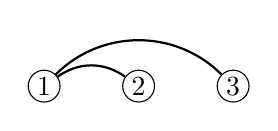
\begin{tikzpicture}[baseline=(n2.base)]
      \node[circle,draw,inner sep=1.2pt] (n1) at (0,0) {$1$};
      \node[circle,draw,inner sep=1.2pt] (n2) at (1.2,0) {$2$};
      \node[circle,draw,inner sep=1.2pt] (n3) at (2.4,0) {$3$};
    
      % same curves, but no arrowheads:
      \draw[line width=0.8pt] (n1) to[bend left=35] (n2);
      \draw[line width=0.8pt] (n1) to[bend left=45] (n3);
    \end{tikzpicture} \Bigg\rangle
    \end{equation}
    This is the same graph as the first one, so the first graph is a GHZ state. We're basically doing Gaussian elimination. 
\end{example}
\begin{example}
    Try yourself:
    \begin{equation}
        \begin{pmatrix}
            Z & Z & I \\
            I & Z & Z \\
            X & X & Y 
        \end{pmatrix}
    \xrightarrow{r_1r_3}
    \begin{pmatrix}
            X & X & Y \\
            Z & Z & I \\
            I & Z & Z 
        \end{pmatrix}
    \xrightarrow{H2S_3}
    \begin{pmatrix}
            X & Z & X \\
            Z & X & I \\
            I & X & Z 
        \end{pmatrix}
    \xrightarrow{H3}
    \begin{pmatrix}
        X & Z & Z \\
        Z & X & I \\
        I & X & X 
    \end{pmatrix}
    \xrightarrow{r_3 \rightarrow r_2r_3}
    \begin{pmatrix}
        X & Z & Z \\
        Z & X & I \\
        Z & Z & X 
    \end{pmatrix}
    \end{equation}
    
\end{example}
Remark: not all states are stabilizer states (ex $\ket{0 + \epsilon}$)\\ 
All states which can be $+1$ eigenstate of a Pauli operator. 
\begin{example}
    5-qubit code state $\ket{+_L}$ \\ 
    \begin{equation}
        \begin{pmatrix}
        X&Z&Z&X&I\\
        I&X&Z&Z&X\\
        X&I&X&Z&Z\\
        Z&X&I&X&Z\\
        X&X&X&X&Y
        \end{pmatrix}
    = \Bigg| 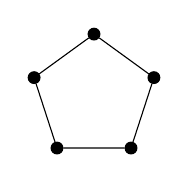
\begin{tikzpicture}[scale=0.4,
  every node/.style={circle, draw, fill=black, inner sep=1.5pt}
]

\node (n1) at (90:2)  {};
\node (n2) at (18:2)  {};
\node (n3) at (-54:2) {};
\node (n4) at (-126:2){};
\node (n5) at (162:2) {};

\draw (n1)--(n2)--(n3)--(n4)--(n5)--(n1);

\end{tikzpicture} \Bigg\rangle\end{equation} 
\end{example}

\begin{example}
    The graph for a 7 qubit code is a graph of half a cube, which is equivalent to 
    \begin{center}
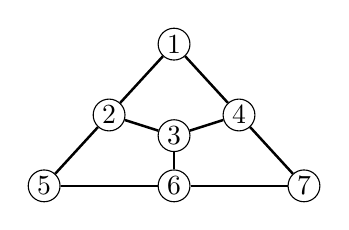
\begin{tikzpicture}[scale=0.75,
  every node/.style={circle, draw, fill=white, inner sep=1.2pt},
  e/.style={line width=0.9pt}
]

% --- triangle corners ---
\node (1) at (0,2.4) {1};
\node (5) at (-2.2,0) {5};
\node (7) at ( 2.2,0) {7};

% --- place 2,4,6 exactly on the triangle sides ---
% 2 on line segment 5--1, 4 on 1--7, 6 on 5--7
\node (2) at (-1.1,1.2) {2};
\node (4) at ( 1.1,1.2) {4};
\node (6) at (0,0) {6};

% interior node
\node (3) at (0,0.85) {3};

% --- outer triangle boundary as segmented sides ---
\draw[e] (5)--(2)--(1);
\draw[e] (1)--(4)--(7);
\draw[e] (5)--(6)--(7);

% --- interior edges (same as the original structure) ---
\draw[e] (2)--(3)--(4);
\draw[e] (3)--(6);

\end{tikzpicture}
\end{center}
\end{example}

Graph state construction circuits
\begin{enumerate}
    \item Each qubit starts in the $\ket{+}=H\ket{0} = $ vertices 
    \item Apply $CZ$-gate ($\Lambda_Z$) for every edge. 
\end{enumerate}
\begin{example}
    The circuit for the GHZ state: 
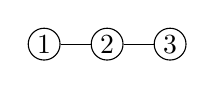
\begin{tikzpicture}[baseline=-0.6ex]
  \node[circle,draw,inner sep=1.2pt] (v1) at (0,0) {$1$};
  \node[circle,draw,inner sep=1.2pt] (v2) at (0.8,0) {$2$};
  \node[circle,draw,inner sep=1.2pt] (v3) at (1.6,0) {$3$};
  \draw (v1) -- (v2) -- (v3);
\end{tikzpicture}

\begin{center}
    \begin{quantikz}
        \lstick{$\ket{0}$} & \gate{H} \slice{$S_0$} & \ctrl{1}  \slice{$S_1$} & \qw \slice{$S_2$}& \qw  \\
        \lstick{$\ket{0}$} & \gate{H} & \ctrl{-1} & \ctrl{1} & \qw\\
        \lstick{$\ket{0}$} & \gate{H} & \qw & \ctrl{-1} & \qw
    \end{quantikz} \\
\end{center}
    Recall:
    \begin{quantikz}
        & \gate{X} & \ctrl{1} & \\
        &  &  \targ & \qw & \qw  
    \end{quantikz} = 
    \begin{quantikz}
        & \ctrl{1} & \gate{X} & \\
        &  \targ{} & \gate{X} &   
    \end{quantikz}
    and 
    \begin{quantikz}
        & \ctrl{1} & \\
        &  \targ{} &  
    \end{quantikz}
    = 
    \begin{quantikz}
        & \qw & \ctrl{1} &  & \\
         & \gate{H} &  \ctrl{-1} & \gate{H} &   
    \end{quantikz} \\
    Therefore, 
    \begin{quantikz}
        & \gate{X} & \ctrl{1} & \\
        &  & \ctrl{-1} & \qw 
    \end{quantikz} = 
    \begin{quantikz}
        & \ctrl{1} & \gate{X} & \\
        &  \ctrl{-1} & \gate{Z} &
    \end{quantikz}
 \\
At $S_0$, $S= \begin{pmatrix}
    X& I &I \\ I &X &I \\ I & I & X
\end{pmatrix}$, $\ket{\psi_0} = \ket{+}\ket{+}\ket{+}$ \\ 
At $S_1$, $S = \begin{pmatrix}
    X& X &I \\ I &Z &I \\ I & I & X
\end{pmatrix}$
At $S_2$, $S = \begin{pmatrix}
    X& Z &I \\ Z & X &I \\ I & I & X
\end{pmatrix}$
At $S_2$, $S = \begin{pmatrix}
    X& Z &I \\ Z & X & Z \\ I & Z & X
\end{pmatrix}$
\end{example}

\begin{theorem}
    $X\text{-}Z$ rule: 
    If you have a graph state and you apply a string of $X$'s to it, then the $X$ will be equivalent to something else in the same graph. 
    \begin{equation}
        X_k \ket{G} = \prod_{j \in neigh(k)} Z_j\ket{G}
    \end{equation}
    ($X$'s will cause a propagation of $Z$'s - just like the following circuit): 
     \begin{quantikz}
        & \gate{X} & \ctrl{1} & \\
        &  & \ctrl{-1} & \qw 
    \end{quantikz} = 
    \begin{quantikz}
        & \ctrl{1} & \gate{X} & \\
        &  \ctrl{-1} & \gate{Z} &
    \end{quantikz}
    The theorem states that bit flip errors can in turn into phase flip errors on a graph state.   
\end{theorem}
Suppose we had a error correction code that corrected possible phase flips, then it would equivalently correct bit flips, and vice-versa. 


\begin{example}
    $X$-$Z$ theorem: \\
    The graph 
    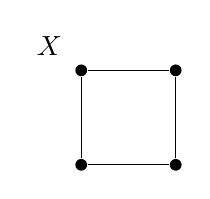
\begin{tikzpicture}[scale=1.2]
  % vertices (square)
  \node[circle,fill=black,inner sep=1.5pt] (v1) at (0,1) {};
  \node[circle,fill=black,inner sep=1.5pt] (v2) at (1,1) {};
  \node[circle,fill=black,inner sep=1.5pt] (v3) at (1,0) {};
  \node[circle,fill=black,inner sep=1.5pt] (v4) at (0,0) {};

  % edges
  \draw (v1)--(v2)--(v3)--(v4)--(v1);

  % label "x" near the top-left vertex
  \node[anchor=south east] at ($(v1)+(-0.1,0.05)$) {$X$};
\end{tikzpicture} 
    is equivalent to 
    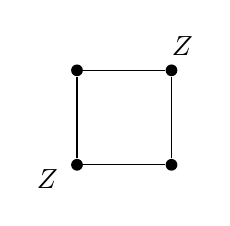
\begin{tikzpicture}[scale=1.2]
  % vertices (square)
  \node[circle,fill=black,inner sep=1.5pt] (v1) at (0,1) {};
  \node[circle,fill=black,inner sep=1.5pt] (v2) at (1,1) {};
  \node[circle,fill=black,inner sep=1.5pt] (v3) at (1,0) {};
  \node[circle,fill=black,inner sep=1.5pt] (v4) at (0,0) {};

  % edges
  \draw (v1)--(v2)--(v3)--(v4)--(v1);

  % label "Z" near the top-left vertex
  \node[anchor=south west] at ($(v2)+(-0.1,0.05)$) {$Z$};
  \node[anchor=north east] at ($(v4)+(-0.1,0.05)$) {$Z$};
\end{tikzpicture} 
\end{example}

This $X$-$Z$ rule led to Codeword Stabilized codes (CWS) codes. This is the to this day the largest systematic construction of non-stabilizing codes.



\subsection{Graph Codes}
(will be going quick because this is not so useful - but conceptually important) \\ 
Goal: Represent subspaces not just states \\
There is a degeneracy in graph representation, because if we flip the sign of any of these generators $g_k \rightarrow -g_k$, we get the same graph. Changing the sign of the generators changes the eigenvalue, like we go from 0 to 1 in a state.  \\
Recall: if $\ket{\psi}$ is a stabilizer state, 
\begin{equation}
    U \ket{\psi} = Ug \ket{\psi} = Ug U^\dagger U \ket{\psi} 
\end{equation}
then $UgU^\dagger$ are stabilizer transforms.

\begin{definition}
    Graph basis for $\ket{G}$ is \begin{equation}
        \{\ket{G_s}= Z^S \ket{G} \,|\, S = \{0,1\}^n \}
    \end{equation} 
    $Z^S$ causes sign change. so for $\ket{G} = \langle g_1, g_2, \ldots, g_n\rangle$, $\ket{G_s} = \langle (-1)^{S_1}g_1, (-1)^{S_2}g_2, \ldots, (-1)^{S_n}g_n\rangle$
\end{definition}

\begin{definition}
    A \textbf{graph code} $C(G,\{S_1,S_2, \ldots\}$ is the space spanned by $\{\ket{GS_1}, \ket{GS_2}, \ldots\}$. 
\end{definition}

\begin{fact}
    Graph codes $\subset$ Stabilizer codes
\end{fact}

\begin{example}
    \begin{equation}
        S = \begin{pmatrix}
            X&I&I \\ I&X&I \\ I&I&X
        \end{pmatrix}
    \end{equation}
    which corresponds to a graph of 3 vertices (no edges)
    $\ket{G} = \ket{+++}$, $Z^{\otimes 3} \ket{G} = \ket{---}$
\end{example}

\begin{example}
    \begin{equation}
        \Bigg| 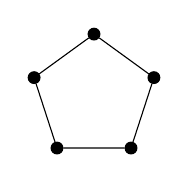
\begin{tikzpicture}[scale=0.4,
  every node/.style={circle, draw, fill=black, inner sep=1.5pt}
]

\node (n1) at (90:2)  {};
\node (n2) at (18:2)  {};
\node (n3) at (-54:2) {};
\node (n4) at (-126:2){};
\node (n5) at (162:2) {};

\draw (n1)--(n2)--(n3)--(n4)--(n5)--(n1);

\end{tikzpicture} \Bigg\rangle = \ket{G}
    \end{equation} and $Z^{\otimes 5} \ket{G} \Rightarrow [[5,1,3]]$ code \\ We only have one qubit.
\end{example}
This gives us a systematic way of getting arbitrary codes. 

\begin{example}
    Shor code graph: \\
    \begin{center}
    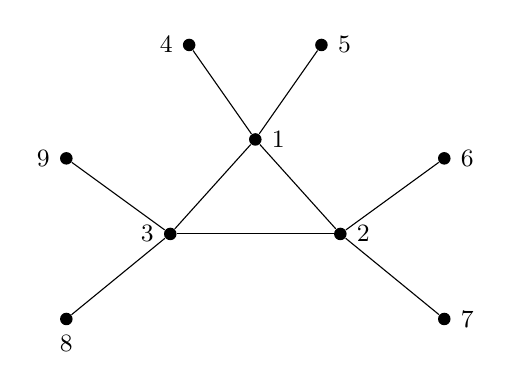
\begin{tikzpicture}[scale=1.2, every node/.style={font=\small}]
  % --- Nodes (positions chosen to match the drawing) ---
  \node[circle, fill=black, inner sep=1.6pt, label=right:$1$] (v1) at (0,1.2) {};
  \node[circle, fill=black, inner sep=1.6pt, label=left:$4$]  (v4) at (-0.7,2.2) {};
  \node[circle, fill=black, inner sep=1.6pt, label=right:$5$] (v5) at (0.7,2.2) {};

  \node[circle, fill=black, inner sep=1.6pt, label=left :$3$] (v3) at (-0.9,0.2) {};
  \node[circle, fill=black, inner sep=1.6pt, label=right:$2$]      (v2) at (0.9,0.2) {};

  \node[circle, fill=black, inner sep=1.6pt, label=left:$9$] (v9) at (-2.0,1.0) {};
  \node[circle, fill=black, inner sep=1.6pt, label=below:$8$] (v8) at (-2.0,-0.7) {};

  \node[circle, fill=black, inner sep=1.6pt, label=right:$6$] (v6) at (2.0,1.0) {};
  \node[circle, fill=black, inner sep=1.6pt, label=right:$7$] (v7) at (2.0,-0.7) {};

  % --- Edges (matching the picture) ---
  \draw (v1)--(v4);
  \draw (v1)--(v5);

  \draw (v1)--(v3);
  \draw (v1)--(v2);

  \draw (v3)--(v2);   % horizontal base edge

  \draw (v3)--(v9);
  \draw (v3)--(v8);

  \draw (v2)--(v6);
  \draw (v2)--(v7);
\end{tikzpicture}
\end{center}
    \hspace*{1.5cm} $=Z_1Z_2Z_3 \ket{G} \Rightarrow [[9,1,3]]$ Shor code.  
\end{example}


\subsection{Surface Codes}
Goal: Define a stabilizer code s.t. if qubits are on a surface, all generators of the code are local operations. \\
Concept: \\
\begin{center}
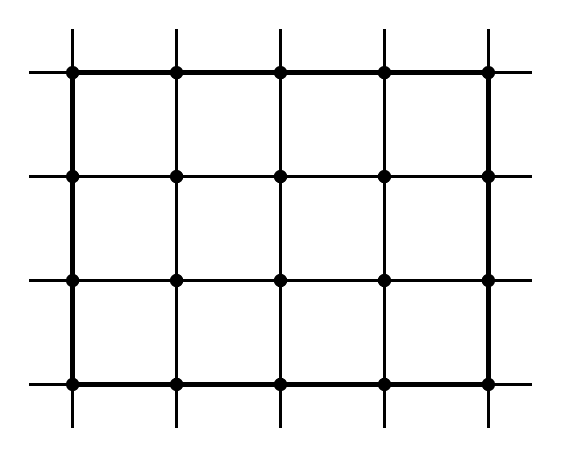
\begin{tikzpicture}[scale=1.1]
  % --- grid size (number of cells) ---
  \def\Nx{4}    % columns of cells
  \def\Ny{3}    % rows of cells
  \def\s{1.2}   % spacing
  \def\ext{0.5}% overshoot amount (in same units as coords)

  % --- draw vertical lines with overshoot ---
  \foreach \i in {0,...,\Nx} {
    \draw[line width=1.2pt]
      (\i*\s,-\ext) -- (\i*\s,\Ny*\s+\ext);
  }

  % --- draw horizontal lines with overshoot ---
  \foreach \j in {0,...,\Ny} {
    \draw[line width=1.2pt]
      (-\ext,\j*\s) -- (\Nx*\s+\ext,\j*\s);
  }

  % --- outer boundary (frame) ---
  \draw[line width=1.8pt] (0,0) rectangle (\Nx*\s,\Ny*\s);

  % --- dots at each intersection (inside the frame) ---
  \foreach \i in {0,...,\Nx} {
    \foreach \j in {0,...,\Ny} {
      \fill (\i*\s,\j*\s) circle (2.2pt);
    }
  }
\end{tikzpicture}
\end{center}

Edges $E$, Vertices $V$, Faces/Plaquette $F/P$;
The qubits be on edges. \\
Periodic boundary conditions = toric code \\
Planar = surface code \\
The goal of all of these constructions is to find a way to represent a stabilizer state, meaning we can write down a series of stabilizer generators which all commute with each other. (This is the fun game with simple rules - just find a systematic way of getting a bunch of stuff commuting and we get a code.) \\

The state generator which will be the products around the edges corresponds to the vertex $v$
\begin{equation}
    A_v = \prod_{e \sim v} X_e \text{ and } B_p =  \prod_{e \sim f} Z_e
\end{equation}

\begin{center}
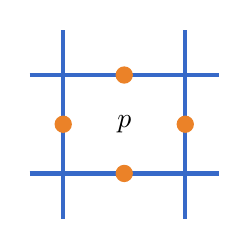
\begin{tikzpicture}[scale=0.5]
  % colors close to the figure
  \definecolor{lineblue}{RGB}{55,105,200}
  \definecolor{dotorange}{RGB}{235,130,40}

  % parameters
  \def\L{2.4}     % half-length of each long line segment
  \def\xs{1.55}   % x-position of the two vertical grid lines
  \def\ys{1.25}   % y-position of the two horizontal grid lines
  \def\r{0.22}    % dot radius

  % grid lines (2 vertical + 2 horizontal)
  \draw[line width=1.5pt, lineblue] (-\xs,-\L) -- (-\xs,\L);
  \draw[line width=1.5pt, lineblue] ( \xs,-\L) -- ( \xs,\L);
  \draw[line width=1.5pt, lineblue] (-\L,-\ys) -- (\L,-\ys);
  \draw[line width=1.5pt, lineblue] (-\L, \ys) -- (\L, \ys);

  % dots (midpoints of each side of the central square)
  \fill[dotorange, line width=1.5pt] (0, \ys)  circle (\r);   % top
  \fill[dotorange, line width=1.5pt] (0,-\ys)  circle (\r);   % bottom
  \fill[dotorange,  line width=1.5pt] (-\xs,0)  circle (\r);   % left
  \fill[dotorange, line width=1.5pt] ( \xs,0)  circle (\r);   % right

  % label
  \node at (0,0) {$p$};
\end{tikzpicture}
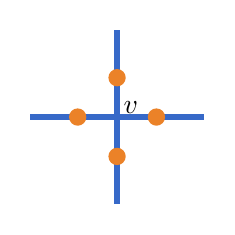
\begin{tikzpicture}[scale=0.5]
  % colors
  \definecolor{lineblue}{RGB}{55,105,200}
  \definecolor{dotorange}{RGB}{235,130,40}

  % parameters
  \def\L{2.2}   % half-length of the cross arms
  \def\r{0.22}  % radius of the dots

  % cross
  \draw[line width=2pt, lineblue] (-\L,0) -- (\L,0);
  \draw[line width=2pt, lineblue] (0,-\L) -- (0,\L);

  % dots (top, bottom, left, right)
  \fill[dotorange,  line width=1.5pt] (0, 1.0) circle (\r);
  \fill[dotorange, line width=1.5pt] (0,-1.0) circle (\r);
  \fill[dotorange, line width=1.5pt] (-1.0,0) circle (\r);
  \fill[dotorange, line width=1.5pt] ( 1.0,0) circle (\r);

  % label
  \node at (0.35,0.25) {$v$};
\end{tikzpicture}
\end{center}


\begin{claim}
    All $B_p, A_v$ commute if they share no qubits, i.e. disjoint. If there's an overlap, they share 2 edges, therefore $B_p, A_v$ commute. We always either share 0 or 2 edges. They commute because the two Pauli operators all multiply out together to give identity. 
\end{claim}

How many qubits are encoded? Let's look at how many degrees of freedom left over. We know that $k = n - |g|$ where $g$ is the number of independent generators. If we take two faces and we take their product: 1) if they're on top of each other, we get the same to each other; 2) if they're adjacent to each other, we get a bigger face; suppose we take all the faces and multiply them together i.e.
\begin{equation}
    \prod_p B_p = \mathbb{1}
\end{equation}
Similarly,
\begin{equation}
    \prod_v A_v = \mathbb{1}
\end{equation}
We have overcounted the number of independent generators. Given an $L \times L$ lattice, 
then 
\begin{align}
    &\text{number of faces } = L^2 \\
    &\text{number of vertices } = L^2 \\
    &\text{number of edges = qubits} = 2L^2
\end{align}
Therefore, 
\begin{equation}
    k = 2L^2 - [L^2 - 1 + L^2 -1] = 2
\end{equation}
where the $-1$ comes from overcounting by 1 since the product is identity. \\
\textit{For the torus code, it is easy to see we have 2 qubits because we have two non-contractible loops that go around the major and minor axis.} \\

Geometry of how these loops work: \\

Imagine if we have two faces next to each other, and we have face $f_1$ and $f_2$. $f_1$ has a $Z$ on the shared qubit and $f_2$ has a $Z$ on the shared qubit. $ZZ = I$, therefore we have 1 larger face.  \\ 

\begin{center}
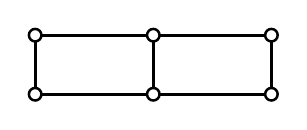
\begin{tikzpicture}[scale=0.75]
  % styles
  \tikzset{
    v/.style={circle, fill=white, draw=black, line width=0.9pt, inner sep=1.6pt},
    e/.style={draw=black, line width=1.2pt}
  }

  % coordinates (two squares sharing the middle vertical edge)
  \coordinate (A) at (0,1);    % top-left
  \coordinate (B) at (2,1);    % top-middle
  \coordinate (C) at (4,1);    % top-right
  \coordinate (D) at (0,0);    % bottom-left
  \coordinate (E) at (2,0);    % bottom-middle
  \coordinate (F) at (4,0);    % bottom-right

  % edges
  \draw[e] (A)--(B)--(C);
  \draw[e] (D)--(E)--(F);
  \draw[e] (A)--(D);
  \draw[e] (B)--(E);
  \draw[e] (C)--(F);
  \draw[e] (D)--(A); % (optional, same as A--D; remove if you want no double-draw)
  \draw[e] (A)--(B)--(E)--(D)--cycle; % left square
  \draw[e] (B)--(C)--(F)--(E)--cycle; % right square

  % vertices
  \node[v] at (A) {};
  \node[v] at (B) {};
  \node[v] at (C) {};
  \node[v] at (D) {};
  \node[v] at (E) {};
  \node[v] at (F) {};
\end{tikzpicture}, $f_1f_2 = $
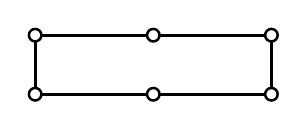
\begin{tikzpicture}[scale=0.75]
  \tikzset{
    v/.style={circle, fill=white, draw=black, line width=0.9pt, inner sep=1.6pt},
    e/.style={draw=black, line width=1.2pt}
  }

  % coordinates (outer rectangle corners + the two middle vertices)
  \coordinate (A) at (0,1);    % top-left
  \coordinate (B) at (2,1);    % top-middle (vertex only)
  \coordinate (C) at (4,1);    % top-right
  \coordinate (D) at (0,0);    % bottom-left
  \coordinate (E) at (2,0);    % bottom-middle (vertex only)
  \coordinate (F) at (4,0);    % bottom-right

  % outer rectangle edges ONLY (no middle vertical line)
  \draw[e] (A)--(C)--(F)--(D)--cycle;

  % vertices (keep all 6)
  \node[v] at (A) {};
  \node[v] at (B) {};
  \node[v] at (C) {};
  \node[v] at (D) {};
  \node[v] at (E) {};
  \node[v] at (F) {};
\end{tikzpicture}
\end{center}

\begin{equation}
    \prod_f B_f^\beta = \text{closed loops of } Z\text{'s } 
\end{equation}


For vertices, if we go through some loop path $\beta$
\begin{center}
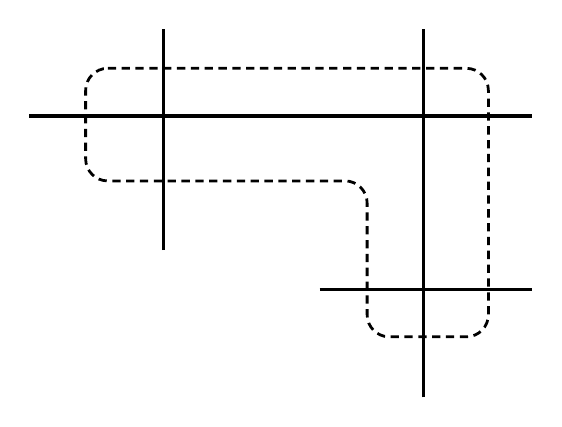
\begin{tikzpicture}[scale=1.1]
  % styles
  \tikzset{
    wire/.style={line width=1.2pt},
    boundary/.style={line width=1.0pt, dashed, dash pattern=on 3pt off 2pt},
    dot/.style={circle, draw, fill=white, inner sep=1.6pt, line width=1pt},
  }

  % junction centers
  \coordinate (A) at (0,1);    % left junction
  \coordinate (B) at (3,1);    % upper-right junction (circled)
  \coordinate (C) at (3,-1);   % lower-right junction

  % main connecting "wires"
  \draw[wire] (A) -- (B);
  \draw[wire] (B) -- (C);

  % draw plus-junctions (little crosses)
  % at A
  \draw[wire] ($(A)+(-1.55,0)$) -- ($(A)+(0.55,0)$);
  \draw[wire] ($(A)+(0,-1.55)$) -- ($(A)+(0,1.)$);

  % at B (plus + circle)
  \draw[wire] ($(B)+(-0.75,0)$) -- ($(B)+(1.25,0)$);
  \draw[wire] ($(B)+(0,-0.75)$) -- ($(B)+(0,1.00)$);

  % at C
  \draw[wire] ($(C)+(-1.20,0)$) -- ($(C)+(1.25,0)$);
  \draw[wire] ($(C)+(0,-1.25)$) -- ($(C)+(0,0.75)$);

  % dashed "L-shaped" boundary with an inner corner
  \draw[boundary, rounded corners=8pt]
    (-0.9, 1.55) -- (3.75, 1.55) -- (3.75,-1.55) -- (2.35,-1.55)
    -- (2.35, 0.25) -- (-0.9,0.25) -- cycle;
\end{tikzpicture}
\end{center}

\begin{equation}
    \prod_v A_v^\beta = \text{closed loops of } X\text{'s in the dual lattice}
\end{equation}

We can contract any loops, except for loops that are topologically non-trivial (like they wind all the way around). How much effort does it take to contract a loop? First, 
\begin{equation}
\text{the number of qubits = number of non-contractable loops}    
\end{equation}
We now have a well defined notion of distance:
\begin{equation}
\text{Distance = length of non-contractable loops}  
\end{equation}
If you imagine that the error is that each one of these edges gets an $X$ or a $Z$ error with some probability $p$, the only time you have an error that would go bad is if you went too far across, and you can't tell if it was actually going all the way around or not, because it becomes misidentified as a non-contractible loop. \\
The loop distance $L\sim \sqrt{n}$, since $n$ goes as $L^2$. So $L$ being the length across the lattice tells you about the number of errors before you start going bad. \\

Scaling properties of when the error correction code would fail: \\
Let $P_{fail}$ be the failure probability rate of decoding (syndrome) and recovery ($R$). 
\begin{equation}
    P_{fail} = C \left(\frac{P}{P_{th}}\right)^{\frac{d+1}{2}}
\end{equation}
where $C$ is a constant that depends on the hardware and decoding error, $P$ is the physical error rate (logical qubit), $P_{th}$ is the property of the code, i.e., the break-even point (threshold probability - will come back to fault-tolerant quantum computing). We can think $P_{th}$ as the number of fault paths in the code decoder. \\
In summary, $P_{th}$ scales with size of code, $P$ has to do with the number of qubits. \\

$d = \#$ physical errors to make non-contractable loop, code can correct up to $t = \frac{d-1}{2}$ errors.  

Matching algorithm: take the syndrome that you get and turn it into the error that you think happened. Perfect matching is an exhaustive way to do that. 
\section{Problem Set 3 - 22 February 2026}
\subsection{Problem 1 - Toric Code: Warmup}
As discussed in lecture, an example of a topological code is the toric code. We can visualize the physical qubits and stabilizers for the $n=18$ toric code via the following interactive diagram (drag to rotate, scroll or use the toolbar to zoom). Edges of the lattice represent physical qubits, blue dots (on vertices of the lattice) represent $X$ stabilizers, and orange dots (on faces) represent $Z$ stabilizers. \\

How many logical qubits are encoded by this code? 2 - this is because there are 2 non-contractable loops. \\
$Z$ operators applied on the red edges (4,5,6) correspond to a logical operator for this code. This is true. \\
Applying $Z$ operators to the red edges (4,5,6) is a distinct operation from applying $Z$ operators to the green edges $(10,11,12)$. This is true.



\newpage
\subsection{Problem 2 - The Toric Code: Syndrome Measurements}
As previously mentioned, the topology and error correction properties of topological codes are closely related. One way to build intuition for this is to examine how syndromes are corrected for in practice. When asked to give a list of stabilizer generators which anticommute with the error (i.e., syndrome measurements), provide your answer as a list of stabilizer indices. 

Assume there are $Z$ errors on the qubits associated with red edges in the following diagrams. For the one in the top left, these are qubits (5, 6, 13); top right, (8, 9, 16); bottom, (5, 6, 10, 11, 12, 13). \\

Measuring a stabilizer corresponding to a face (orange dot) will reveal an error has occurred in any of the above: this is false. \\

Syndrome indices for the top left diagram: \\
Syndrome indices for the top right diagram: \\
Syndrome indices for the bottom diagram: \\



\newpage
\subsection{Problem 3 - Decoherence free spaces and stabilizers}
Quantum error correction is an example of “active" error correction where one first detects whether an error occurs and then applies a correcting operation. An interesting area of research in quantum information is the possibility of “passive" error correction. We explore in this problem one of these possibilities, Decoherence Free Subspaces (DFS), in the context of stabilizer codes.

Recall the following: If $S$ is the stabilizer for the code $C$, then $\forall V \in S$, and $\forall \ket{\psi} \in C$, $V\ket{\psi = \ket{\psi}}$.

As an example, consider the three qubit bit flip code, $C_{bf}$, where $\ket{0_L} = \ket{000}$ and $\ket{1_L} = \ket{111}$. The stabilizer $S$ is generated by $ZZI$ and $IZZ$, that is $S = \langle ZZI, IZZ \rangle$ 

The code can correct error $E$ if $E$ is a Pauli group element which anticommutes with at least one of the generators of the code.  
 
Give the stabilizer generators which anticommute with each of the following errors.
\begin{itemize}
    \item $E_1 = XII$, then $S = \langle ZZI\rangle$
    \item $E_1 = IXI$, then $S = \langle ZZI, IZZ\rangle$
    \item $E_1 = IIX$, then $S = \langle IZZ\rangle$
    \item $E_4 = ZIZ$, then $S = \emptyset$
\end{itemize}




\newpage
\subsection{Problem 4 - Topological QEC - A Projective Plane Code}
Quantum error correction codes can be constructed using graphs on topological surfaces, where vertices and faces correspond to certain stabilizer operations, and the distance of the code is given by the shortest non-trivial topological chain of errors. In this problem, we explore a specific instance of such a construction, on a projective plane. \\

The projective plane in two dimensions, $\mathfrak{R}P^2$, can be drawn as a disc in which antipodal points on the boundary are identified. Recall that a cellulation $\mathcal{C}$ of a surface defines sets $F$, $E$, and $V$ of faces, edges, and vertices. For each $e \in E$, there corresponds a qubit on which $X_e$ and $Z_e$ are the Pauli $X$ and $Z$ operators. Let $E_f \subset E$ be the set of edges around face $f \in F$, and let $E_v \subset E$ be the set of edges attached to vertex $v \in V$. For the set of all $f$ and $v$, we define
\begin{align}
    A_f &= \bigotimes\limits_{e \in E_f} Z_e \\
    B_v &= \bigotimes\limits_{e \in E_v} X_e \\
\end{align}
The set of all $A_f$ and $B_v$ is the stabilizer for the code. We want to find a list of stabilizers for the following (three $A_f$ and single unique $B_v$ for the cellulation: 

\begin{center}
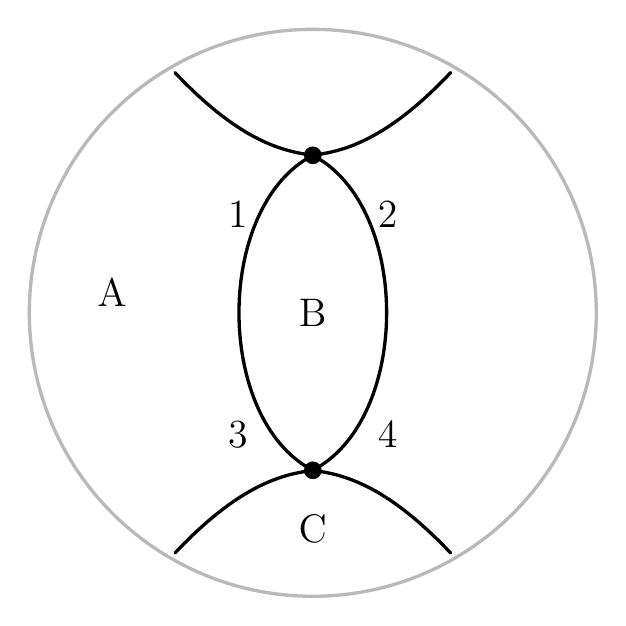
\begin{tikzpicture}[scale=1, line cap=round, line join=round]

% --- Parameters (adjust to taste) ---
\def\R{3.6}        % outer radius
\def\ytop{2.0}     % y of top black dot
\def\ybot{-2.0}    % y of bottom black dot
\def\xbulge{1.25}  % half-width of the B-oval

% --- Outer circle ---
\draw[gray!55, line width=1.2pt] (0,0) circle (\R);

% --- Top cap boundary curve (a smooth arc) ---
\draw[line width=1.2pt]
  (-1.75,3.05)
  .. controls (-0.9,2.15) and (-0.35,2.05) .. (0,\ytop)
  .. controls (0.35,2.05) and (0.9,2.15) .. (1.75,3.05);

% --- Central region B boundary (vertical oval made of two Beziers) ---
\draw[line width=1.2pt]
  (0,\ytop)
  .. controls (-\xbulge,1.35) and (-\xbulge,-1.35) .. (0,\ybot);
\draw[line width=1.2pt]
  (0,\ytop)
  .. controls (\xbulge,1.35) and (\xbulge,-1.35) .. (0,\ybot);

% --- Bottom cap boundary curve (a smooth arc) ---
\draw[line width=1.2pt]
  (-1.75,-3.05)
  .. controls (-0.9,-2.15) and (-0.35,-2.05) .. (0,\ybot)
  .. controls (0.35,-2.05) and (0.9,-2.15) .. (1.75,-3.05);

% --- Black nodes (dots) ---
\fill (0,\ytop) circle (3.2pt);
\fill (0,\ybot) circle (3.2pt);

% --- Labels ---
\node at (-2.55,0.25) {\Large A};
\node at (0,0.0)      {\Large B};
\node at (0,-2.75)    {\Large C};

% --- Edge numbers ---
\node at (-0.95,1.25) {\Large 1};
\node at ( 0.95,1.25) {\Large 2};
\node at (-0.95,-1.55){\Large 3};
\node at ( 0.95,-1.55){\Large 4};

\end{tikzpicture}
\end{center}


This code acts on four qubits ($|E| = 4$), corresponding to the four edges, labeled $1$ through $4$. Note there are only three distinct faces, labeled $A$, $B$, and $C$. These stabilizers must commute with each other.\\

There are 3 face stabilizers: \\
\begin{itemize}
    \item For face A: $ZZZZ$
    \item For face B: $ZZII$
    \item For face C: $IIZZ$
\end{itemize}
There are 2 vertices, however they both give the same stabilzer: $XXXX$ \\
Therefore the stabilizers are:
\begin{equation}
    [ZZZZ,ZZII,IIZZ,XXXX]
\end{equation}



\newpage
\subsection{Problem 5 - Topological QEC - A Projective Plane Code II}
In problem 4, we want to find out the states that they stabilize. The list of stabilizers from Problem 4 is 
\begin{equation}
    [ZZZZ,ZZII,IIZZ,XXXX]
\end{equation}
Then the states they stabilize are:
\begin{align}
    \ket{0_L} = \ket{0000} + \ket{1111} \\
    \ket{0_L} = \ket{0011} + \ket{1100} 
\end{align}


\newpage
\subsection{Problem 6 - Topological QEC - Another Projective Plane Code}
Quantum error correction codes can be constructed using graphs on topological surfaces, where vertices and edges correspond to certain stabilizer operations, and the distance of the code is given by the shortest non-trivial topological chain of errors. In this problem, we explore a specific instance of such a construction, on a projective plane.\\

The projective plane in two dimensions, $\mathfrak{R}P^2$, can be drawn as a disc in which antipodal points on the boundary are identified. Recall that a cellulation $\mathcal{C}$ of a surface defines sets $F$, $E$, and $V$ of faces, edges, and vertices. For each $e \in E$, there corresponds a qubit on which $X_e$ and $Z_e$ are the Pauli $X$ and $Z$ operators. Let $E_f \subset E$ be the set of edges around face $f \in F$, and let $E_v \subset E$ be the set of edges attached to vertex $v \in V$. For the set of all $f$ and $v$, we define
\begin{align}
    A_f &= \bigotimes\limits_{e \in E_f} Z_e \\
    B_v &= \bigotimes\limits_{e \in E_v} X_e \\
\end{align}
The set of all $A_f$ and $B_v$ is the stabilizer for the code. We want to find a list of stabilizers for the following cellulation:

\begin{center}
    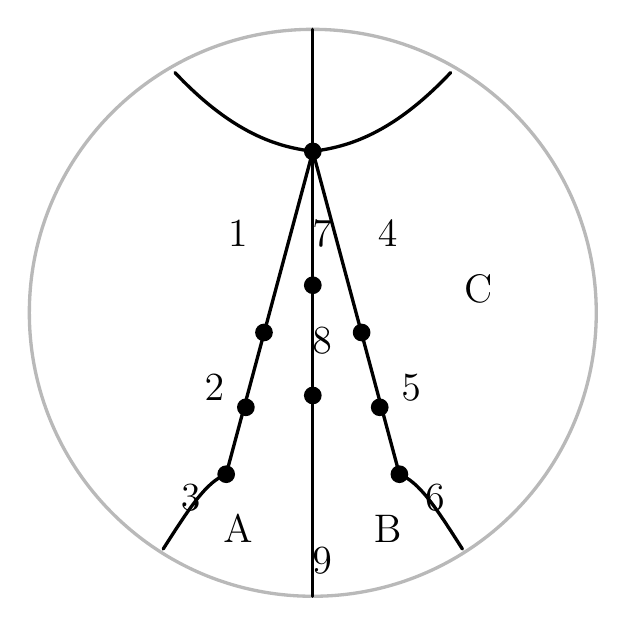
\begin{tikzpicture}[scale=1, line cap=round, line join=round]

% ----------------- Parameters (tweak to match perfectly) -----------------
\def\R{3.6}          % outer radius
\def\ytop{2.05}      % y-position of the apex dot
\def\capx{1.75}      % half-width of the top cap arc endpoints (x)
\def\capy{3.05}      % y of the top cap arc endpoints

% Key points
\coordinate (O)    at (0,0);
\coordinate (Top)  at (0,\R);
\coordinate (Bot)  at (0,-\R);

\coordinate (P)    at (0,\ytop);         % apex dot
\coordinate (L3)   at (-1.10,-2.05);     % lower-left slanted endpoint (dot)
\coordinate (R6)   at ( 1.10,-2.05);     % lower-right slanted endpoint (dot)

% Intermediate dots on slanted edges
\coordinate (L2)   at (-0.85,-1.20);
\coordinate (L1)   at (-0.62,-0.25);
\coordinate (R5)   at ( 0.85,-1.20);
\coordinate (R4)   at ( 0.62,-0.25);

% Dots on the center vertical line
\coordinate (C7)   at (0,0.35);
\coordinate (C8)   at (0,-1.05);

% Bottom arc endpoints (where the small arcs meet the outer circle)
\coordinate (BL)   at (-1.90,-3.00);
\coordinate (BR)   at ( 1.90,-3.00);

% ----------------- Outer circle -----------------
\draw[gray!55, line width=1.2pt] (O) circle (\R);

% ----------------- Top cap arc + top vertical segment -----------------
\draw[line width=1.2pt]
  (-\capx,\capy)
  .. controls (-0.95,2.20) and (-0.35,2.10) .. (P)
  .. controls ( 0.35,2.10) and ( 0.95,2.20) .. (\capx,\capy);

% vertical line from top of circle to apex
\draw[line width=1.2pt] (Top) -- (P);

% ----------------- Central vertical line (down to bottom) -----------------
\draw[line width=1.2pt] (P) -- (Bot);

% ----------------- Slanted boundaries -----------------
\draw[line width=1.2pt] (P) -- (L3);
\draw[line width=1.2pt] (P) -- (R6);

% ----------------- Bottom curved arcs (A and B boundaries) -----------------
\draw[line width=1.2pt]
  (BL) .. controls (-1.55,-2.45) and (-1.35,-2.15) .. (L3);
\draw[line width=1.2pt]
  (BR) .. controls ( 1.55,-2.45) and ( 1.35,-2.15) .. (R6);

% ----------------- Dots -----------------
\foreach \pt in {P,L1,L2,L3,R4,R5,R6,C7,C8}
  \fill (\pt) circle (3.2pt);

% ----------------- Region labels -----------------
\node at (-0.95,-2.75) {\Large A};
\node at ( 0.95,-2.75) {\Large B};
\node at ( 2.10, 0.30) {\Large C};

% ----------------- Edge/segment numbers -----------------
\node at (-0.95, 1.00) {\Large 1};
\node at (-1.25,-0.95) {\Large 2};
\node at (-1.55,-2.35) {\Large 3};

\node at ( 0.95, 1.00) {\Large 4};
\node at ( 1.25,-0.95) {\Large 5};
\node at ( 1.55,-2.35) {\Large 6};

\node at ( 0.12, 1.00) {\Large 7};
\node at ( 0.12,-0.35) {\Large 8};
\node at ( 0.12,-3.15) {\Large 9};

\end{tikzpicture}
\end{center}

For the 3 faces: Face A: $A_1 = ZZZIIIZZZ$, Face B: $A_2 = IIIZZZZZZ$, Face C: $A_3 = ZZZZZZIII$

For the 7 vertices:
\begin{itemize}
    \item Vertex 7: $B_1 = XIXXIXXIX$
    \item Vertex 1: $B_2 = XXIIIIIII$, Vertex 3: $B_3 = IXXIIIIII$
    \item Vertex 4: $B_4 = IIIXXIIII$, Vertex 6: $B_5 = IIIIXXIII$
    \item Vertex 8: $B_6 = IIIIIIXXI$, Vertex 9: $B_7 = IIIIIIIXX$
\end{itemize}



\newpage
\subsection{Problem 7 - Topological QEC - Another Projective Plane Code II}
The dimension of the vector space stabilized by these stabilizers is given by $2^{n-m}$. Here $n = 9$. We want to find the number of independent stabilizer generators. \\

There are 3 faces $A$, $B$, $C$, hence 3 operators $A_f$, but they satisfy $A_AA_BA_C = I$ because every edge appears in the boundary of exactly two faces (so every $Z_e$ appears twice and cancels). Therefore the number of independent face stabilizers is: 3-1 = 2 \\

There are 9 vertices, but from the  antipodal identification
\begin{itemize}
    \item 1 top vertices (edges 1,4,7 meet)
    \item 2 vertices on the left branch (one between edges 1-2, and one between edges 2-3)
    \item 2 vertices on the right branch (one between edges 4-5, and one between edges 5-6)
    \item 2 vertices on the central branch (one between edges 7-8, and one between edges 8-9)
\end{itemize}
Therefore we have 7 vertices. But the satisfy $B_1 B_2\cdots B_7 = I$. Therefore, the number of independent vertex stabilizers is $7-1=6$. \\

Therefore there are a total of $m$ independent stabilizers. \\

The dimension of the vector space stabilzed by these stabilizers is then given by $2^{9-8} = 2$. 


\newpage
\subsection{Problem 8 - Toric code on $3x3$ lattice}
Recall that the toric code had stabilizer generators
\begin{equation}
    B_f = \prod_{e\sim f} Z_e \text{ and } A_v = \prod_{e\sim v} X_e
\end{equation}
for faces $f$ and vertices $v$. Measuring these generators produces the syndromess, and once syndromes of the code are measured, we may process this data using classical routines to determine the recovery operation needed to be applied to fix errors. However, there is a great deal of flexibility in the classical routine we choose! In this problem, we will explore one such routine for the toric code and analyze its performance in a random error model. \\

We study a toric code on a $3\times 3$ square lattice. Define coordinates for the vertices so that $(0,0)$ is the bottom left vertex. Label coordiates for the faces so that $(1/2, 1/2)$ is the bottom face: 

\begin{center}
    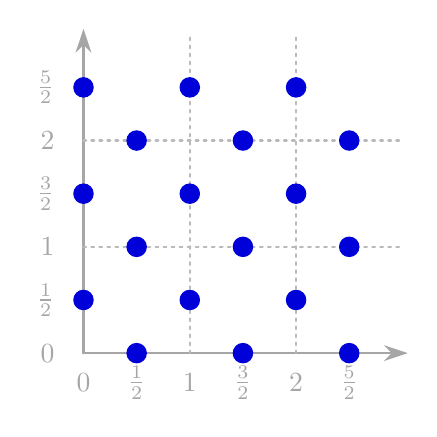
\begin{tikzpicture}[scale=1.35, line cap=round, line join=round]

% --- Axes ---
\draw[-{Stealth[length=3mm,width=2mm]}, gray!70, line width=0.9pt] (0,0) -- (3.05,0);
\draw[-{Stealth[length=3mm,width=2mm]}, gray!70, line width=0.9pt] (0,0) -- (0,3.05);

% --- Dotted guide lines (as in the picture) ---
\draw[gray!55, dotted, line width=0.9pt] (1,0) -- (1,3);  % x=1
\draw[gray!55, dotted, line width=0.9pt] (2,0) -- (2,3);  % x=2
\draw[gray!55, dotted, line width=0.9pt] (0,1) -- (3,1);  % y=1
\draw[gray!55, dotted, line width=0.9pt] (0,2) -- (3,2);  % y=2

% --- Points (blue) ---
\tikzset{pt/.style={circle, fill=blue!85!black, draw=blue!85!black, inner sep=0pt, minimum size=7pt}}

% x = 0 column: y = 1/2, 3/2, 5/2
\node[pt] at (0,0.5) {};
\node[pt] at (0,1.5) {};
\node[pt] at (0,2.5) {};

% x = 1/2 column: y = 0,1,2
\node[pt] at (0.5,0) {};
\node[pt] at (0.5,1) {};
\node[pt] at (0.5,2) {};

% x = 1 column: y = 1/2, 3/2, 5/2
\node[pt] at (1,0.5) {};
\node[pt] at (1,1.5) {};
\node[pt] at (1,2.5) {};

% x = 3/2 column: y = 0,1,2
\node[pt] at (1.5,0) {};
\node[pt] at (1.5,1) {};
\node[pt] at (1.5,2) {};

% x = 2 column: y = 1/2, 3/2, 5/2
\node[pt] at (2,0.5) {};
\node[pt] at (2,1.5) {};
\node[pt] at (2,2.5) {};

% x = 5/2 column: y = 0,1,2
\node[pt] at (2.5,0) {};
\node[pt] at (2.5,1) {};
\node[pt] at (2.5,2) {};

% --- Tick labels (fractions like the figure) ---
% x-axis labels at 0, 1/2, 1, 3/2, 2, 5/2
\node[gray!70] at (0,-0.28) {$0$};
\node[gray!70] at (0.5,-0.28) {$\frac12$};
\node[gray!70] at (1,-0.28) {$1$};
\node[gray!70] at (1.5,-0.28) {$\frac32$};
\node[gray!70] at (2,-0.28) {$2$};
\node[gray!70] at (2.5,-0.28) {$\frac52$};

% y-axis labels at 0, 1/2, 1, 3/2, 2, 5/2
\node[gray!70, anchor=east] at (-0.18,0) {$0$};
\node[gray!70, anchor=east] at (-0.18,0.5) {$\frac12$};
\node[gray!70, anchor=east] at (-0.18,1) {$1$};
\node[gray!70, anchor=east] at (-0.18,1.5) {$\frac32$};
\node[gray!70, anchor=east] at (-0.18,2) {$2$};
\node[gray!70, anchor=east] at (-0.18,2.5) {$\frac52$};

\end{tikzpicture}
\end{center}



Note that we also identify the top and bottom edges and the left and right edges to form a 2-torus, and recall that qubits (depicted as blue dots in the above figure) are positioned on edges.

\begin{enumerate}
    \item Syndrome operators are associated with a vertex or a face. Suppose the error $X_{(1/2,0)} \otimes Y_{(1,1/2)} \otimes Y_{1,3/2} \otimes Z_{2,3/2}$ happens. Which syndrome operators anticommute with this error? Give a list of the vertices and faces corresponding to these syndrome operator. \\

    We look for faces touching edges with $X$ or $Y$. 
    \begin{itemize}
        \item Horizontal edge (1/2,0) touches faces: (1/2, 1/2) and (1/2,5/2)
        \item Vertical edge (1,1/2) touches faces (1/2, 1/2) and (3/2,1/2) 
        \item Vertical edge (1,3/2) touches faces (1/2, 3/2) and (3/2, 3/2)
    \end{itemize}

    Now we count parity by face: 
    \begin{itemize}
        \item Face (1/2, 1/2) touches (1/2,0)$\rightarrow X$ and (1,1/2)$\rightarrow Y$; That is 2 X-components, an even number which means it commutes
        \item Face (1/2, 5/2) touches (1/2, 0) $\rightarrow 1 \rightarrow$ anticommutes
        \item Face (3/2, 1/2) touches (1,1/2) $\rightarrow 1 \rightarrow$ anticommutes
        \item Face (1/2, 3/2) touches (1,3/2) $\rightarrow 1 \rightarrow$ anticommutes
        \item Face (3/2, 3/2) touches (1,3/2) $\rightarrow 1 \rightarrow$ anticommutes
    \end{itemize}
    Therefore, the 4 face syndromes are $[(1/2,5/2), (3)]$
\end{enumerate}




\newpage
\subsection{Problem 9 - Syndrome decoding for random errors - recovery}




\newpage
\subsection{Problem 10 - Syndrome decoding for random errors - correctness}




\newpage
\subsection{Problem 11 - Matching algorithm performance}




\newpage
\subsection{Problem 12 - Matching algorithm performance II}




\newpage
\subsection{Problem 13 - Matching algorithm performance III}
%%%%% Week 4 %%%%% 
\section{Quantum Error Correction Midterm Review - 23 February 2026}
\subsection{Preliminaries}
Gates: 
\begin{itemize}
    \item Hadamard \begin{quantikz} & \gate{H} &\end{quantikz} $\frac{1}{\sqrt{2}}\begin{pmatrix} 1 & 1 \\ 1 & -1 \end{pmatrix}$
    \item Pauli-X \begin{quantikz} & \gate{X} &\end{quantikz} $\begin{pmatrix} 0 & 1 \\ 1 & 0 \end{pmatrix}$
    \item Pauli-Y \begin{quantikz} & \gate{Y} &\end{quantikz} $\begin{pmatrix} 0 & -i \\ i & 0 \end{pmatrix}$
    \item Pauli-Z \begin{quantikz} & \gate{Z} &\end{quantikz} $\begin{pmatrix} 1 & 0 \\ 0 & -1 \end{pmatrix}$
    \item Phase \begin{quantikz} & \gate{S} &\end{quantikz} $\begin{pmatrix} 1 & 0 \\ 0 & i \end{pmatrix}$
    \item $\pi/8$ \begin{quantikz} & \gate{T} &\end{quantikz} $\begin{pmatrix} 1 & 0 \\ 0 & e^{i\pi/4} \end{pmatrix}$
\end{itemize}
Matrix Multiplications:
\begin{itemize}
    \item $X\ket{0} = \ket{1}, X\ket{1} = \ket{0}$, $Y\ket{0} = i\ket{1}, Y\ket{1} = -i\ket{0}$, $Z\ket{0} = \ket{0}, Z\ket{1} = -\ket{1}$
    \item $HXH = Z$, $HZH = X$, $HYH = -Y$
    \item $SXS^\dagger = Y$, $SYS^\dagger = X$, $SZS^\dagger = Z$   
\end{itemize}

\subsection{Lecture 1: Introduction, Quantum Circuits and Density Matrices}

\subsection{Introduction}
Quantum Mechanics Postulates: 1) States: Quantum system = unit vector $=k\ket{\psi}$, 2) Gates: $\ket{\psi'} = U\ket{\psi}$, 3) Measurement: collection of $\{M_m\}$ of measurement operators. The index $m$ refers to the measurement outcomes, probability is given by $p(m) = \braket{\psi|M_k|\psi}$ , 4) Composition: Tensor Product (many qubits)  \\


\subsubsection{Quantum Circuits, Density Matrices}
Density matrices: Suppose we have $\ket{\psi}$ or $\ket{\phi} $ with probability $\frac{1}{2}$? The density matrix is given by $\rho = \frac{1}{2} \ketbra{\psi} + \frac{1}{2} \phi$. \\

Suppose
\begin{quantikz}
    \makeebit{$\ket{\psi}_{AB}$} & \wire[l][1]["A"{above,pos=0.3}]{a} & \rstick{state?} \\
            & \wire[l][1]["B"{above,pos=0.3}]{a}& \meter{}
\end{quantikz}
Let $\ket{\psi}_{AB} = \sqrt{\frac{3}{4}} \ket{00} + \sqrt{\frac{1}{4}} \ket{11}$. Suppose $B$ measures their state, $A$'s state is a statistical mixture: We get either $\sqrt{\frac{3}{4}} \ket{0}$ or $\sqrt{\frac{1}{4}} \ket{1}$. \\
Suppose we now apply a Hadamard to $B$ before we measure. Then the state after the Hadamard is $\frac{1}{\sqrt{2}}[\sqrt{\frac{3}{4}}\ket{0}(\ket{0} + \ket{1}) + \sqrt{\frac{1}{4}}\ket{1}(\ket{0} - \ket{1})].$ When $B$ measures a $\ket{0}$, then $A$ sees $\sqrt{\frac{3}{4}}\ket{0} + \sqrt{\frac{1}{4}}\ket{1}$. When $A$ measures a $\ket{1}$, then $A$ sees $\sqrt{\frac{3}{4}}\ket{0} - \sqrt{\frac{1}{4}}\ket{1}$. \\
These two matrices are the same statistical mixtures by calculating the density matrices. We can use the definition of density matrix:
\begin{equation}
    \rho = \sum_k \ketbra{\psi_k}
\end{equation}

\begin{definition}
    Density matrix $\rho$ is a density matrix iff $\Tr(\rho) = 1$ and $\rho \geq 0$, i.e. $\forall \ket{\phi}$, $\braket{\phi|\rho|\phi} \geq 0$ and is real. 
\end{definition}

\begin{claim}
    \begin{equation}
        \rho = \sum_k \ketbra{\psi_k}
    \end{equation}
    where $p_k$ is a probability distribution. \\
    Proof: $\Tr(\rho) = \sum p_k = 1$, and $\braket{\phi|\rho|\phi} = \braket{\phi|\psi_k}^2 \geq = 0$
\end{claim}

\begin{claim}
    Any $\rho$ can be expressed as stochastic combination of pure states$\sum_k p_k \ketbra{\psi_k}$ \\
    Proof: $\rho$ is positive and thus has a spectral decomposition. $\rho = \sum_k \lambda_k \ketbra{k}$. The trace is $\sum \lambda_k = 1$ where $\lambda$ is a probability distribution and real. 
\end{claim}

\begin{definition}
    $\rho$ is pure iff $\rho = \ketbra{\psi}$, otherwise $\rho$ is mixed
\end{definition}

Is $\rho = \sum_k p_k \rho_k$ a legal density matrix? Yes!

\begin{lemma}
    von Neumann unravellings: \\
    Let $\rho = \sum_k p_k \ketbra{\psi_k}$. Then $\rho = \rho' = q_k \ketbra{\phi_k}$ if 
    \begin{equation}
        \sqrt{p_k} \ket{\psi_k} = \sum_j U_{kj}\sqrt{q_j}\ket{\phi_j}
    \end{equation}
    (doesn't matter what basis $B$ measures in)
\end{lemma}

\begin{definition}
    A purification of $\rho_A$ is a state $\ket{\psi_{AB}}$ s.t. 
    \begin{equation}
        \rho_A = \Tr_B \ketbra{\psi_{AB}}
    \end{equation}
    where $\Tr_B$ is the partial trace (can be viewed as the circuit earlier. 
\end{definition}


\subsection{Lecture 2: Quantum Operations}
\subsubsection{System-environment model}
Goal: describe all ways in which an $\rho_{in} \xrightarrow{\mathcal{E}} \rho_{out}$, where $\mathcal{E}$ is a map. \\
Model: Suppose 
\begin{center}
\begin{quantikz}
    \lstick{$\ket{\psi}$} & \gate[2]{U} & \rstick{$\rho_{out}$? } \\
    \lstick{$\ket{e}$} &  & \meter{}
\end{quantikz} 
\end{center}
where $\ket{e}$ is the environment and the meter is the is the measurement operators $\ketbra{e_0}, \ketbra{e_1}, \ldots$. \\
\begin{equation}
    \ket{e}\ket{\psi} \rightarrow U \ket{e}\ket{\psi}
\end{equation}
Let $\oplus$ be ``or". Then:
\begin{align}
    \rho &= \braket{e_0|U|e} \oplus \braket{e_1|U|e} \oplus \cdots \\
    &= \oplus_k \braket{e_k|U|e} \ket{\psi}
\end{align}
$E_r = \braket{e_k|U|e}$ is called an ``operation element" or a Krauss operator, or error operator.
\begin{equation}
    \rho_{out} = \sum_k E_k \rho E_k^\dagger = \mathcal{E}(\rho) \quad \text{where } \sum_k E_kE_k^\dagger = I 
\end{equation}
This setup with the system-environment model giving us an equation that maps the input density matrix with an output density matrix is important idea for quantum error correction. 

\subsubsection{Quantum operations - definition and criteria}
In general, what is legal $\rho \rightarrow \mathcal{E}(\rho)$? 
\begin{definition}
    $\mathcal{E}$ is a valid quantum operation iff 
    \begin{enumerate}
        \item Trace preserving $\Tr[\mathcal{E}(\rho)] = 1$
        \item Convex and linear: $\mathcal{E}(\sum_k p_k\rho_k) = \sum p_k \mathcal{E}(\rho_k)$ where $p_k$ are probability distribution
        \item Complete positivity: a) if $\rho \geq 0 \Rightarrow \mathcal{E}(\rho) \geq 0$; b) $(I_R \otimes \mathcal{E}_Q)(\rho_{RQ}) \geq 0$ if $\rho_{RQ} \geq 0$
    \end{enumerate}
\end{definition}


\subsubsection{Operator Sum Representation}
\begin{theorem}
    Let 
    \begin{equation}
    \mathcal{E}(\rho) = \sum_k E_k \rho E_k^\dagger = \mathcal{E}(\rho) \quad \text{where } \sum_k E_kE_k^\dagger = I 
\end{equation}
$\mathcal{E}(\rho)$ is a valid quantum operation.
\end{theorem}
Check if this is true. \\
Thus, for all 
\[
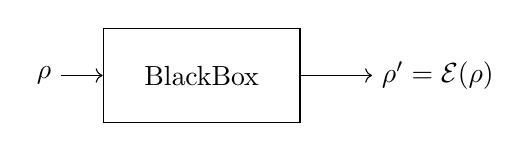
\begin{tikzpicture}[baseline=(current bounding box.center)]
    % Nodes
    \node (rho) at (0,0) {$\rho$};
    \node[draw, minimum width=2.5cm, minimum height=1.2cm] (box) at (2,0) {Black\\Box};
    \node (rho2) at (5,0) {$\rho' = \mathcal{E}(\rho)$};
    
    % Arrows
    \draw[->] (rho) -- (box);
    \draw[->] (box) -- (rho2);
\end{tikzpicture}
\qquad
\text{for some } \{\mathcal{E}_k\}
\]
For all black boxes taking $\rho$ to $\rho' = \mathcal{E}(\rho)$ there will exist a set of quantum operation elements  $\{E_k\}$ to describe any such black box transformation.
Additionally, there exists a system-environment model for any quantum operation $\mathcal{E}$. 
\begin{center}
\begin{quantikz}
    \lstick{$\ket{\psi}$} & \gate[2]{U} & \rstick{$\rho' = \mathcal{E}(\rho)$   } \\
    \lstick{$\ket{e}$} &  & \meter{}
\end{quantikz} 
\end{center}
Due to the fact that we can measure in any basis $E_k$'s are not necessarily unique. 

\begin{example} Operator Sum Representation\\
    \begin{enumerate}
        \item 
        \begin{quantikz}
            & \gate{U} &    
        \end{quantikz} then $\mathcal{E}(\rho) = U\rho U^\dagger$

        \item Let $\{P_k\}$ be projectors
        \begin{quantikz}
            & \meter{} &    
        \end{quantikz} then $\mathcal{E}(\rho) = \sum_k P_k \rho P_k^\dagger$

        \item 
        \begin{quantikz}
            \lstick{$\rho$} & \ctrl{1} & & \rstick{$\mathcal{E}(\rho)$} \\
            \lstick{$\ket{0}$} & \gate{R_y(\theta)} & \meter{}
        \end{quantikz} where the controlled $R_y(\theta)$ is the black box. Recall $R_y = \begin{pmatrix} \cos\frac{\theta}{2} & -\sin\frac{\theta}{2} \\ \sin\frac{\theta}{2} & \cos\frac{\theta}{2} \end{pmatrix}$. Let $\lambda = \sin^2 \frac{\theta}{2}$. Let $e$ be the first qubit and $s$ be the second qubit. Then,
        \begin{equation}
            U = \begin{pmatrix}
                1 & 0 & 0 & 0 \\
                0 & \sqrt{1-\lambda} & 0 & -\lambda \\
                0 & 0 & 1 & 0 \\
                0 & \sqrt{\lambda} & 0 & \sqrt{1-\lambda}
            \end{pmatrix}
        \end{equation}
        Recall $E_k = \braket{e_k|U|e}$. This is not a number but an operator that acts on the system qubit. We can read out of $U$ by looking at the matrix elements that are 0 for the environment qubit which is the upper left box.
        \begin{equation}
            E_0 = \braket{0|U|0} = \begin{pmatrix}1 & 0 \\ 0 & \sqrt{1-\lambda} \end{pmatrix}
        \end{equation}
        similarly, $E_1$ is given by the bottom left matrix. 
        $E_1 = \braket{1|U|0} = \begin{pmatrix}0 & 0 \\ 0 & - \lambda \end{pmatrix}$. \\

        This operation is an important physical process called phase damping. We can see this by applying it to an arbitrary density matrix. 
        \begin{align}
            \mathcal{E}(\rho) &= E_0\rho E_0^\dagger + E_1\rho E_1^\dagger \\
            &= \begin{pmatrix}a & b \\ b^*\sqrt{1-\lambda} & c\sqrt{1-\lambda}\end{pmatrix} E_0^\dagger + \begin{pmatrix}0 & 0 \\ b^* & c\lambda \end{pmatrix} E_1 \\
            &= \begin{pmatrix}a & b\sqrt{1-\lambda} \\ b^*\sqrt{1-\lambda}  & c(1-\lambda)\end{pmatrix} + \begin{pmatrix}0 & 0 \\ 0 & c\lambda \end{pmatrix} \\
            &= \begin{pmatrix}a & b\sqrt{1-\lambda} \\ b^*\sqrt{1-\lambda}  & c\end{pmatrix}
        \end{align}
        If $\sqrt{1-\lambda}$ is an exponentially decaying function in time, often in real practice. $\sqrt{1-\lambda} \rightarrow e^{-t/T_2}$, where $T_2$ is the phase damping time. 

        \item 
        \begin{quantikz}
            \lstick{$\rho$} & \ctrl{1} &  \targ{} &  &\rstick{$\mathcal{E}(\rho)$} \\
            \lstick{$\ket{0}$} & \gate{R_y(\theta)} & \ctrl{-1}& \meter{}
        \end{quantikz} where the controlled $R_y(\theta)$ and controlled-NOT is the black box. \\
        $E_0$ stays the same because the environment does not change only when the system qubit is in the $\ket{0}$ state. The second CNOT does nothing
        \begin{equation}
            E_0 = \braket{0|U|0} = \begin{pmatrix}1 & 0 \\ 0 & \sqrt{1-\lambda} \end{pmatrix}
        \end{equation}
        For $E_1$, the operation element is the same as before, except that an $X$ and not gate has to happen. 
        \begin{equation}
            E_1 = \braket{1|U|0} = \begin{pmatrix} 0 &1 \\ 1 & 0 \end{pmatrix} \begin{pmatrix}0 & 0 \\ 0 & - \lambda \end{pmatrix} = \begin{pmatrix}0 & \sqrt{\lambda} \\ 0 & 0 \end{pmatrix}
        \end{equation}
        This is called amplitude damping. If we apply this to an arbitrary density matrix.
        \begin{equation}
            \mathcal{E}(\rho) = \begin{pmatrix}
                1 - c(1-\lambda) & b\sqrt{1 - \lambda} \\ b^*\sqrt{1-\lambda} & c(1-\lambda) = \begin{pmatrix}
                    1 - ce^{-t/T_1} & b1 - be^{-t/2T_1} \\
                    b^*1 - ce^{-t/2T_1} & ce^{-t/T_1}
                \end{pmatrix}
            \end{pmatrix}
        \end{equation}
        Diagonal decay such that the left top element goes to 1, and the bottom right element goes to 0. Diagonal term decay is the loss of energy of the system, that is the amplitude decay. Note that $T1=2T_2$ which is the loss of energy from a qubit. 
    \end{enumerate}
\end{example}


\subsubsection{Unitary degree of freedom in OSR}
There are infinite choices of $\{E_k\}$ to give the same $\mathcal{E}$.
\begin{center}
\begin{quantikz}
    \lstick{$\ket{\psi}$} & \gate[2]{U} && \rstick{$\rho' = \mathcal{E}(\rho)$   } \\
    \lstick{$\ket{e}$} &  & \gate{U'} & \meter{}
\end{quantikz} 
\end{center}
We can change the basis of the environment before measuring. 
\begin{lemma}
    If $\{E_k\}$ describe a valid operator sum representation $\mathcal{E}$. then $F_j = \sum_k U_{jk}E_k$ describes the same $\mathcal{E}$. \\
    Proof: 
    \begin{equation}
        \sum_j F_j \rho F_j^\dagger = \sum_{jkk'}U_{jk}E_k\rho E_{k'}^\dagger U_{jk'}^* = \sum_{kk'} = \delta_{kk'}E_k\rho E_k^\dagger = \mathcal{E}
    \end{equation}
\end{lemma}


\subsection{Lecture 3: Quantum Error Correction}
\subsubsection{Classical Coding}
Error model: Let the left 0,1 be the sender and the right 0,1 be the receiver. 
\[
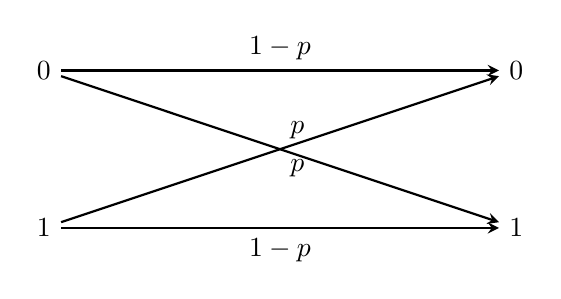
\begin{tikzpicture}[>=stealth, thick]

% Left labels
\node (l0) at (0,2) {$0$};
\node (l1) at (0,0) {$1$};

% Right labels
\node (r0) at (6,2) {$0$};
\node (r1) at (6,0) {$1$};

% Straight arrows (no flip)
\draw[->] (l0) -- node[above] {$1-p$} (r0);
\draw[->] (l1) -- node[below] {$1-p$} (r1);

% Cross arrows (flip)
\draw[->] (l0) -- node[midway, above right] {$p$} (r1);
\draw[->] (l1) -- node[midway, below right] {$p$} (r0);

\end{tikzpicture}
\]
The probability of error is given by $prob(error) = p$. This channel is symmetric and is known as the``binary symmetric channel". 

\begin{definition}
    A classical $[n,k,d]$ code is a set of $2^k$ $n$-bit strings with minimum Hamming distance $d$. 
\end{definition}

\begin{definition}
    $d(x,y) = w(x \oplus y ) = $ Hamming distance where $\oplus$ is bitwise $XOR$ and $w$ is the number of $1$'s (weight)
\end{definition}

\begin{example}
    $000 \rightarrow o_L$ and $111 \rightarrow 1_L$; thus $n=3$, $k=1$, $d=3$. Therefore, $[n,k,d] = [3,1,3]$ \\

    Suppose the sender sends $000 = 0_L$, then apply the binary symmetric channel with probability $p$. What the receiver sees as a result of this error can be written as a stochastic mixture of a certain set of received states
    
    \begin{center}
    \begin{tabular}{ c | c | c }
    Receive & Probability & Decode\\
    \hline
    000 & $(1-p)^3$ & 0 \\
    001 & $p(1-p)^2$ & 0 \\
    010 & $p(1-p)^2$ & 0 \\
    100 & $p(1-p)^2$ & 1 \\
    011 & $p^2(1-p)$ & 1 \\
    101 & $p^2(1-p)$ & 1 \\
    111 & $p^3$ & 1 \\
    \end{tabular}
    \end{center}
    The last 4 rows show that an error has occurred.\\
    The probability of error is given by
    \begin{align}
        Prob(err) = p^3 + 3p^2(1-p) = 3p^2 + 2p^3 = O(p^2)
    \end{align}
    which is lower than the original channel error probability which had $O(p)$. Thus this is an effective way of correcting errors. 
\end{example}


\subsubsection{Quantum Coding}
Circa 1995: Impossible because
\begin{enumerate}
    \item States collapse when measured
    \item Errors are continuous
    \item No-cloning (no redundancy code)
\end{enumerate}
We now get around it by
\begin{enumerate}
    \item Do not measure state holding quantum info - only measure environment
    \item Orthogonal using entanglement
    \item Orthogonal using entanglement
\end{enumerate}

Quantum bit-flip code: \\
Suppose $\mathcal{E}(\rho) = (1-p)\rho + p X \rho X$ ``bit-flip channel" \\
Schematically, 
\begin{center}
\begin{quantikz}
    \lstick{Alice} & \gate{\mathcal{E}(\rho)} & \rstick{Bob} 
\end{quantikz} 
\end{center}
\begin{definition}
    An $[[n,k]]$ quantum code $C$ is a $k$-qubit subspace of an $n$-qubit Hilbert space. 
\end{definition}
\begin{example}
    $n=3, k=1, \ket{000} = \ket{0_L}, \ket{111} = \ket{1_L}$ \\
    naive way of doing it is $a\ket{0} + b\ket{1} \rightarrow (a\ket{0} + b\ket{1})^{\otimes 3}$ but is not possible due to no cloning theorem. \\
    Returning to $\mathcal{E}(\rho) = (1-p)\rho + P X \rho X$. Let $\psi = a\ket{000} + b\ket{111}$
    \begin{center}
    \begin{tabular}{ c | c}
    Receive & Probability \\
    \hline
    $a\ket{000} + b\ket{111}$ & $(1 -p)^3$  \\  
    $a\ket{001} + b\ket{110}$ & $p(1-p)^2$  \\  
    $a\ket{010} + b\ket{101}$ & $p(1-p)^2$  \\  
    $a\ket{100} + b\ket{001}$ & $p(1-p)^2$  \\  
    $a\ket{011} + b\ket{100}$ & $p^2(1-p)$  \\  
    $a\ket{101} + b\ket{010}$ & $p^2(1-p)$  \\  
    $a\ket{100} + b\ket{001}$ & $p^2(1-p)$  \\  
    $a\ket{111} + b\ket{000}$ & $p^3$ 
    \end{tabular}
    \end{center}
    The last 4 states, and error has occurred. The first 4 states are mutually orthogonal, so in principle distinguishable. Error correction should be possible by projecting it onto these orthogonal subspace
\end{example}


\subsubsection{Operator measurement and error syndromes}
Given $U$ has eigenvalues $\pm 1$, and eigenvectors $\ket{\pm U}$, ``measuring U" is: \\
\begin{quantikz}
    \lstick{$\ket{0}$} & \gate{H} \slice{$\phi_0$}& \ctrl{1} \slice{$\phi_1$}& \gate{H} \slice{$\phi_2$}& \meter{Z} \\
    \lstick{$c_0\ket{u_+} + c_1 \ket{u_-}$} & & \gate{U} & & \rstick{$\ket{\psi}$}
\end{quantikz}
\begin{align}
    \ket{\phi_0} &= \frac{\ket{0} + \ket{1}}{\sqrt{2}}[c_0 \ket{u_+} + c_1 \ket{u_-}] \\
    \ket{\phi_1} &=  \frac{\ket{0}}{\sqrt{2}}[c_0 \ket{u_+} + c_1 \ket{u_-}] + \frac{\ket{1}}{\sqrt{2}}[c_0 \ket{u_+} - c_1 \ket{u_-}] \\
    \ket{\phi_2} &=  \frac{\ket{0} + \ket{1}}{\sqrt{2}}[c_0 \ket{u_+} + c_1 \ket{u_-}] + \frac{\ket{0}-\ket{1}}{\sqrt{2}}[c_0 \ket{u_+} - c_1 \ket{u_-}] \\
     &=  \ket{0}c_0 \ket{u_0} + \ket{1} c_1 \ket{u_-}
\end{align}
If we measure $Z=0$, the state is $\ket{\psi} = \ket{u_+}$, and if we measure $Z =1$, the state is $\ket{\psi} = \ket{u_-}$\\



Error correction and Syndrome Measurements

Operation measurement is thus seen as a projector into the $\pm 1$ eigenvalue subspaces of a unitary operator. This is extremely useful for error. Specifically, we will employ operator measurement to obtain the error syndrome. The error syndrome tells us what error has occurred, that is the effect of the environment will be determined by syndrome operators. 

\begin{enumerate}
    \item measure ``syndrome" ops\\
    For the 3-qubit bit-flip code, these are the two syndrome operators: $U_1 = ZZI$ and $U_2 = IZZ$ \\
    Recall the measurement results obtained when the syndrome operators are measured: $ZZI\ket{000} = + \ket{000}$ and $ZZI\ket{111} = (-1 \ket{1})(-1\ket{1})\ket{1}= + \ket{111}$ Therefore, $U_1(a\ket{000} + \ket{b}\ket{111}) = \ket{a}\ket{000} + b\ket{111}$ which has a $+1$ eigenstate which means $m=0$. $U_2\ket{001} = IZZ \ket{001} = -\ket{001}$, $U_2\ket{110} = -\ket{110}$ \\
    We can make the following statement:
    \begin{equation}
        ZZ\ket{xy} = \begin{cases}
            \ket{xy} \text{ if even \#1's} \\
            -\ket{xy} \text{ if odd \#1's} \\
        \end{cases}
    \end{equation}
    Therefore, $U_2(a\ket{001} + \ket{b}\ket{110}) =  -(\ket{a}\ket{001} + b\ket{110})$

\begin{center}
    \begin{tabular}{ c | c | c | c | c | c}
    Receive & Probability & $U_1=ZZI$ & $U_2=IZZ$ & Recovery $R$ & State\\
    \hline
    $a\ket{000} + b\ket{111}$ & $(1 -p)^3$ & 0 & 0 & $I$ & $a\ket{000} + b\ket{111}$\\  
    $a\ket{001} + b\ket{110}$ & $p(1-p)^2$ & 0 & 1 & $X_3$ &$ a\ket{000} + b\ket{111}$\\ 
    $a\ket{010} + b\ket{101}$ & $p(1-p)^2$ & 1 & 1 & $X_2$ & $a\ket{000} + b\ket{111}$\\
    $a\ket{100} + b\ket{001}$ & $p(1-p)^2$ & 1 & 0 & $X_1$ & $a\ket{000} + b\ket{111}$ \\
    $a\ket{011} + b\ket{100}$ & $p^2(1-p)$ & 0 & 1 & $X_3$ & $a\ket{111} + b\ket{000}$\\
    $a\ket{101} + b\ket{010}$ & $p^2(1-p)$ & 1 & 1 & $X_2$ & $a\ket{111} + b\ket{000}$\\
    $a\ket{100} + b\ket{001}$ & $p^2(1-p)$ & 1 & 0 & $X_1$ & $a\ket{111} + b\ket{000}$\\
    $a\ket{111} + b\ket{000}$ & $p^3$ & 0 & 0 & $I$ & $a\ket{111} + b\ket{000}$
    \end{tabular}
\end{center}
\item Apply unitary ``recovery operation" $R$\\ 
$R$ conditioned on syndrome. The result of this recover operation recovers original qubit. This is for single qubit errors. \\

If two errors occurred, we can also get the syndrome measurements. We then get the inverted qubit
$a\ket{111} + b\ket{000}$, the wrong state. \\
    
\end{enumerate}

How good is the error corrected state?:\\
Fidelity: $F= \rho, \ket{\psi}^2 = \braket{\psi|\rho|\psi} \geq 1 -3p^2(1-p) - p^3 = 1 - 3p^2 + 2p^3 = 1 - O(p^2)$. Without quantum error correction this fidelity would have gone as $1-O(p)$. This is a significant improvement, and this is a signature of quantum error correction. \\

Three qubit bit-flip QEC example overall circuit: \\
\begin{center}
\begin{quantikz}
 \wireoverride{n} &  \wireoverride{n} & \wireoverride{n} & \wireoverride{n} \lstick{$\ket{0}$} & \gate{H} & \ctrl{1} & \ctrl{2} & \gate{H} & \meter{m_0} & \cw & \cwbend{1} \\ 
\lstick{$a\ket{0} + b\ket{1}$} & \ctrl{1}  & \ctrl{2} & \gate{\mathcal{E}_{BF}} & \qw  & \gate{Z} & \qw  & \qw  & \qw & \qw & \gate[wires=3]{R} & \qw \\
\lstick{$\ket{0}$} & \targ{} &\qw & \gate{\mathcal{E}_{BF}} & \qw & \qw & \gate{Z} & \gate{Z} & \qw  &\qw  & & \qw \\
\lstick{$\ket{0}$} &   \qw & \targ{} & \gate{\mathcal{E}_{BF}} & \qw & \gate{Z} & \qw & \qw & \qw  & \qw & & \qw \\
 \wireoverride{n} &  \wireoverride{n} & \wireoverride{n} & \wireoverride{n} \lstick{$\ket{0}$} & \gate{H} & \ctrl{-1} & \qw & \ctrl{-2} & \gate{H} & \meter{m_1} & \cwbend{-1} \\ 
\end{quantikz}
\end{center}
The output is $a\ket{000} + b\ket{111}$ with high fidelity. \\

\begin{claim}
    This scheme can also correct a small rotation error! \\
    Proof: $\mathcal{E}(\rho) = e^{-i \epsilon X_1} \rho e^{i \epsilon X_1}$, where $e^{-i \epsilon X_1} = R_{x1}(2\epsilon)$. Then $\mathcal{E}\ket{\psi} = R_{x1}(2\epsilon) \ket{\psi} \simeq \ket{\psi} - i \epsilon X_1 \ket{\psi}$. When no error correction is applied, the fidelity of this output is is the overlap $F = \sqrt{\norm{\braket{\psi|\psi'}}^2} \geq 1- \epsilon$. When error correction is applied, something different happens due to the syndrome measurement. The syndrome measurement causes the superposition of error or no error to collapse. Thus we obtain $\ket{\psi}$ or $-i\epsilon X_1 \ket{\psi}$ where $\epsilon X$ has a bit flip error applied to it. There is no continuous error cases. We either have error or no error and thus the recovery operator applied to the error channel output state gives us a fidelity which to leading error gives us $F(R(\mathcal{E}(\ket{\psi}))) \geq \sqrt{1 - \epsilon^4} \simeq 1 - \epsilon^2$. This is the same improvement as the full quantum error correction circuit. Therefore, the scheme corrects for a small rotation error. 
\end{claim}




\subsubsection{Correcting quantum errors}
Bit flip channel: $\mathcal{E}_{bf}(\rho) = (1-p)\rho + pX\rho X$ ``classical" errors\\ 
Phase flip channel: $\mathcal{E}_{pf}(\rho) = (1-p)\rho + pZ\rho Z$ quantum! \\

Review the bit-flip code: the code word is $\ket{\psi} = a\ket{000} + b\ket{111} = a\ket{0_L} + b\ket{1_L}$. How do we correct phase errors. Recall $H = \frac{1}{\sqrt{2}} = \begin{pmatrix} 1 & 1 \\ 1 & -1 \end{pmatrix}$, $HXH=Z$, and $HZH = X$. Thus
\begin{equation}
    H \mathcal{E}_{bf}(H\rho H) H = \mathcal{E}_{pf}
\end{equation}
Let $\ket{\pm} = \frac{\ket{0} \pm \ket{1}}{\sqrt{2}}$. The the phase flip code is 
\begin{equation}
    \ket{\psi} = c_1 \ket{+++} + b\ket{---}
\end{equation}
where $\ket{+++} = \ket{0_L}$ and $\ket{---} = \ket{1_L}$. Note that $\mathcal{E}_{pf}: \ket{-} \Leftrightarrow \ket{+}$. \\
Phase flip circuit: 
\begin{center}
    \begin{quantikz}
        \lstick{$a\ket{0}+ b\ket{1}$} & \ctrl{1} & \ctrl{2} & \gate{H} & \gate[3]{\mathcal{E}_{pf}}^{\otimes 3} & \gate{H} & \\
        \lstick{$\ket{0}$} & \targ{} & & \gate{H} & & \gate{H} & \rstick{......}\\
        \lstick{$\ket{0}$} &  & \targ{} & \gate{H} & &\gate{H} & 
    \end{quantikz}
\end{center}
Where the circuit is the same syndrome measurements and recovery operations as we did for the 3-qubit bit flip code. 
\begin{claim}
    Arbitrary qubit errors can be represented as $X$, $Z$, $XZ$ errors. \\
    Proof: Recall $\mathcal{E}(\rho) = \sum_k E_k \rho E_k^\dagger$. Recall $Y = \begin{pmatrix}
        0 & -i \\ i & 0 
    \end{pmatrix} = i XZ$. Let $\sigma_j = \{I,X,Y,Z\}$ and $E_k = \sum_j c_{jk}\sigma_j$. Then 
    \begin{equation}
        \mathcal{E}(\rho) = \sum_{kjj'} c_{kj}c_{kj'} \sigma_j \rho \sigma_{j'} = \sum_{jj'} \sigma_j \rho \sigma_{j'}
    \end{equation}
\end{claim}

\begin{example}
    Recall $R_x(2\epsilon) \ket{\psi} \simeq \ket{\psi} - i \epsilon X \ket{\psi}$. Then 
    \begin{equation}
        \mathcal{E}(\rho) = \rho - i\epsilon(X\rho - \rho X) + \epsilon^2 X\rho X
    \end{equation}
    The second term disappears in the syndrome measurement. In particular, what the syndrome measurement does in general removes all these off-diagonal terms in the $\chi$ matrix representation. The syndrome measurement projects the environment into a definite action given action by Pauli matrix namely, $\{X,Y,Z\}$ as the error
\end{example}


\subsubsection{Shor's 9-qubit code}
Codewords for Shor's 9-qubit code:
\begin{align}
    \ket{0_L} & = \frac{(\ket{000} + \ket{111})^{\otimes 3}}{\sqrt{8}} \\
    \ket{1_L} & = \frac{(\ket{000} - \ket{111})^{\otimes 3}}{\sqrt{8}}
\end{align}
This code can correct for any single qubit error. \\
Syndromes and recovery procedure:
\begin{align}
    \ket{0_L} & = (\ket{0_10_20_3} + \ket{1_11_21_3})(\ket{0_40_50_6} + \ket{1_41_51_6})(\ket{0_70_80_9} + \ket{1_71_81_9}) \\
    \ket{1_L} & = (\ket{0_10_20_3} - \ket{1_11_21_3})(\ket{0_40_50_6} - \ket{1_41_51_6})(\ket{0_70_80_9} - \ket{1_71_81_9}) 
\end{align}

For the bit-flip errors: 
\begin{align}
    Z_1Z_2 &\quad Z_2Z_3\\ 
    Z_4Z_5 &\quad Z_5Z_6\\ 
    Z_7Z_8 &\quad Z_8Z_9 
\end{align}
Phase-flip errors:
\begin{align}
    X_1X_2X_3X_4X_5X_6 \\
    X_4X_5X_6X_7X_8X_9
\end{align}
For bit flips, the parity check operators check the pairs of all possible qubits in each one of these triplets for errors. Why are there 3 copies? This is evident from phase flip operators. For phase flips it checks for sign parity between the pairs. 9-qubit code concatenates a bit flip code and a phase flip code. \\

Performance:\\
\# of possible errors: Identity + ($X,Y,Z$ and 9 qubits) $ = 1 + 3\cdot 9 = 28$\\
\# of possible syndrome values: we have 6 possible bit flip syndrome values, and 2 possible phase flip values.,Thus we have $2^8 = 256$ distinguishable errors. Thus, this code can correct some two qubit errors! 

\begin{definition}
    A perfect $[[n,k]]$ code has $\log_2(1+3n)$ syndrome operators.
\end{definition}
\begin{example}
    $[[5,1]]$ code. There are $1 + 3\cdot 5 = 16$ errors, and we have 4 syndrome errors, thus we have $2^4 = 16$ syndrome values. Thus the 5 qubit code is perfect. 
\end{example}



\subsection{Lecture 4: Stabilizer and CSS codes}
\subsubsection{Quantum Error Correction Criteria}
Quantum Error Correction Criteria:\\
Let the channel be $\mathcal{E}(\rho) = \sum_k E_k \rho E_k^\dagger$. 
\begin{theorem}
    Let $C$ be a quantum code defined by the projector $P = \sum_l \ketbra{\psi_l}$. There exists a quantum operation, a recovery and syndrome measurement $R$ which corrects a certain set of errors defined by $\mathcal{E}$ on the subspace $C$ iff 
    \begin{equation}
        PE_k^\dagger E_j P = d \delta_{jk} P
    \end{equation}
    $E_k^\dagger E_j $ denotes the relationship of the two errors $E_k$ and $E_j$. \\
    Equivalently, 
    \begin{equation}
        \braket{\psi_l|E_j^\dagger E_k|\psi_l} = 0, \forall j \neq k, \forall l 
    \end{equation}
    The off-diagonal terms talk about $E_j$ and $E_k$ and say they must be orthogonal for all errors which are different from each other and for all codeword states. This is the \textbf{orthogonality} criterial. For the on-diagonal element 
    \begin{equation}
        \braket{\psi_l|E_k^\dagger E_k|\psi_l} = d_k, \forall l
    \end{equation}
    That is, it must not distinguish codewords. This is the \textbf{non-deformation} criterion. 
\end{theorem}
When these algebraic conditions are satisfied, $R$ exists, and can be also be found using the proof of these conditions. \\
Proof: Intuition: There's a Hilbert space with a subset $C$. This codeword space has as its image under error operators $E$ some transform vector space. For example, $E$ may transform to a smaller or displaced version of itself. Another different error may also map $C$ into an image. If that image collides with the image of the first operator $E$, then we cannot distinguish these two images from each other. Collisions like this are ruled out by the orthogonality. If the images. If the images are all orthogonal and thus distinguishable, the second error correction criterion requires that images not be deformed, that is, an error operator cannot differentially change one basis state by a length that is different from how another basis state is changed. That is the non-deformation criterion. \\

The recovery operator should thus distinguish these image subspace and unshrink them to recover the original by polar decomposition. By polar decomposition, each one of the error operators may be written as $E_k P = U_k \sqrt{PE_k^\dagger E_k P}$, where $u_k$ is the phase portion, i.e. the rotation, and the magnitude is portion is $PE_k^\dagger E_k P$. From the error correction criteria, we know that $PE_k^\dagger E_k P = d_k$. Summarizing,
\begin{equation}
    E_kP = U_k \sqrt{PE_k^\dagger E_k P} = \sqrt{d_k}U_k P 
\end{equation}
The two parts of the recovery operation are first a syndrome measurement and second a rescaling. \\
\begin{enumerate}
    \item Syndrome measurement: We want to project into the $k$th image of the code word space. Let $p_k = U_kPu_k^\dagger = \frac{E_kPu_k^\dagger}{\sqrt{d_k}} = \frac{u_kPE_k^\dagger}{\sqrt{d_k}}$ \\
    By QEC Criteria: $PE_k^\dagger E_jP = d_k \delta_{jk} P$, the $P_k$ are orthogonal to each other: 
    \begin{equation}
        \forall k \neq j\! P_kP_j \propto U_kPE_k^\dagger E_jPu_j^\dagger = 0 
    \end{equation}This is expected since we required that the images of $C$ be orthogonal to each other. and $P_k$ project into the image of $C$. \\
    Thus the recovery operator : measure $P_k$ which gives $k$ as the syndrome for the error. \\

    Given the syndrome for the error, we now want to recover the initial state.

    \item Recovery: Perform $U_k^\dagger$ which undoes the rotation caused by $E_k$. 
    \begin{equation}
        R(\rho) = \sum_k U_k^\dagger P_k \rho P_k U_k
    \end{equation}
    The overall recovery operation combines the syndrome measurement $P_k$. The post-syndrome measurement $\rho'= P_k\rho P_k$. \\
    For a state $\ket{\psi} \in C$, 
    \begin{equation}
        U_k^\dagger P_kE_j \ket{\psi} = \ket{\psi}
    \end{equation}
     where $E_j\ket{\psi}$ is the erroneous state (error on code), $P_k$ is the syndrome measurement operation, $U_k^\dagger$ is the recovery operation which rotates the state back, ideally gives us $\psi$. Check:
     \begin{align}
         U_k^\dagger P_kE_j \ket{\psi} &= \frac{U_k^\dagger U_k P E_k^\dagger E_j}{\sqrt{d_k}} \ket{\psi} \\
         &= \frac{U_k^\dagger U_k P E_k^\dagger E_jP_k}{\sqrt{d_k}} \ket{\psi} \qquad \text{can insert $P$ since $P\ket{\psi} \in C$} \\ 
         &= \frac{d_k}{\sqrt{d_k}} \delta_{jk} \ket{\psi}
     \end{align}
     Thus,
     \begin{align}
         R(\mathcal{E}(\ketbra{\psi})) &= R(\sum_j E_j \ketbra{\psi}E_j^\dagger) \\
         &= \sum_{kj} U_k^\dagger P_kE_j \ketbra{\psi} E_j^\dagger P_jU_k \\
         &=\sum_{jk}d_k \delta_{jk} \ketbra{\psi} \\W
         &= \ketbra{\psi}\sum_k d_k \\
         &= \ketbra{\psi}
     \end{align}
    Where $\sum_k d_k = 1$ by $\sum_k = E_k^\dagger E_k = I$. 
\end{enumerate}


\subsubsection{Classical linear codes}
An important concept in classical coding theory is tools to generate families of codes with useful parameters. 
\begin{definition}
    A linear $[n,k,d]$ error correcting code is a $2^k$ $n$-bit strings which are closed under (binary) addition. (note: $0\dots0$ always a codeword). 
\end{definition}
We have already seen an example of a linear code: namely the three-bit repetition code or in fact any repetition code. The reason linear codes are so interesting is because they can be described by a smaller set of generators. 

\begin{definition}
    The $n \times k$ generator matrix $G$ encodes data $\Vec{x}$ into the code word space via matrix multiplication $\Vec{v} = G\Vec{x}$. Columns of $G$ are basis codewords. (Linear multiplication generates the code word states)
\end{definition}
\begin{example}
    \begin{equation}
        G = \begin{pmatrix}
            1 \\ 1 \\ 1
        \end{pmatrix}, \qquad G \begin{pmatrix}
            0
        \end{pmatrix} = \begin{pmatrix}
            0 \\ 0 \\ 0
        \end{pmatrix}, \qquad  G \begin{pmatrix}
            1
        \end{pmatrix} = \begin{pmatrix}
            1 \\ 1 \\ 1
        \end{pmatrix}
    \end{equation}
    These correspond to logical 0 and logical 1. 
\end{example}
Linear codes also offer a very straightforward way to determine when an error has occurred and what the error is. This is done by the parity check matrix. 
\begin{definition}
    The parity check matrix $H$ is an $(n-k) \times n$ matrix such that $H \vec{v} = 0, \forall v \in C$. ($H$ annihilates code words). Equivalently, $HG= 0$. 
\end{definition}
\begin{example}
    Repetition Code:
    \begin{equation}
        H = \begin{pmatrix}
            1 & 1 & 0 \\ 0 & 1 & 1
        \end{pmatrix}
    \end{equation}
    It checks the parity of the first two qubits and the last two qubits. Rows of $H$ are orthogonal to columns of $G = \begin{pmatrix}1 & 1 & 1 \end{pmatrix}^T$. \\
    If $\vec{v}$ is corrupted by some string $\vec{e}$, $\vec{v} \rightarrow \vec{v} + \vec{e}$, then when $H (\vec{v} + \vec{e})= H \vec{e} = $ syndrome. Under certain circumstances this error syndrome will be unique and allow $\vec{e}$ to be uniquely determined. 
\end{example}
Note that the code words constrain columns of $H$. 
\begin{lemma}
    If code has distance $d$, then $H$ has at least d linearly independent columns. 
\end{lemma}
In the 3-bit repetition code, 
\begin{equation}
\begin{pmatrix}
    1 & 1 & 0 \\ 0 & 1 & 1
\end{pmatrix} \begin{pmatrix}
    1 \\ 1 \\ 1
\end{pmatrix} = 0
\end{equation}
The sum of columns = 0. \\
\begin{equation}
\end{equation}

\begin{example}
    For $d=3$, no 2 columns of $H$ should be the same. 
\end{example}
\begin{example}
    Hamming codes: for $r \geq 2$, let $H$ cols $= 2^r - 1$ as bit strings $\in \{0,1\} \neq 0$. \\
    For $r=2$, we get the 3-bit repetition code. \\
    For $r=3$, 
    \begin{equation}
        H = \begin{pmatrix}
            0 & 0 & 0 & 1 & 1 & 1 & 1 \\
            0 & 1 & 1 & 0 & 0 & 1 & 1 \\
            1 & 0 & 1 & 0 & 1 & 0 & 1
        \end{pmatrix}    
    \end{equation}
    This 7-bit Hamming code has parameters $[7,4,3]$\\
    In general, $n=2^r - 1$ and $k = n-r$. \\
    The generator $G$ may be constructed by taking the transpose of a matrix, which takes $H$ and adds an additional row of 1's
    \begin{equation}
        H = \begin{pmatrix}
            1 & 1 & 1 & 1 & 1 & 1 & 1 \\
             &  &  & H &  &  &  \\
             &  &  &  &  &  & 
        \end{pmatrix}^T    
    \end{equation}
    Recall $G$ must have columns orthogonal to the rows of $H$. Note that every row of $H$ has four 1's and note that rows of $H$ are orthogonal to each other and this is why $G$ has this structure. 
\end{example}
For quantum codes, we will later need a specific kind of classical linear code. 
\begin{definition}
    Let code $C$ be $[n,k]$ with given generator $G$ and parity check matrix $H$. Define $C^\perp$ is the code with generator $H^T$ and parity check matrix $G^T$. The code words of $C^\perp$ are orthogonal to those of $C$. Therefore we may call $C^\perp$ the dual code to those of $C$. 
\end{definition}
\begin{lemma}
    If $x \in C^\perp$ is given then $\sum_y in C$, then
    \begin{equation}
        \sum_{y \in C} (-1)^{x\cdot y} = \norm{c}
    \end{equation}
    Otherwise,
    \begin{equation}
        \sum_{y \in C} (-1)^{x\cdot y} = 0
    \end{equation}
\end{lemma}


\subsubsection{Stabilizers}
\begin{definition}
    The Pauli group $G_n$ on $n$-qubits $=$ all $n$-fold tensor products of $\{X,Y,Z\}$ and $\{\pm 1, \pm i\}$. 
\end{definition}
\begin{example}
    For $n=1$ qubit, $G = \{I, X,Y, Z, \ldots \}$. 
\end{example}
Note: for $g,h \in G$, either $gh=hg$ or $gh=-hg$. 
\begin{definition}
    For a given vector subspace $V_s \doteq \{\ket{\psi_l}\}$, a stabilizer is the set $S = \{g \in G \! | \! g \ket{\psi} = \ket{\psi} \forall \ket{\psi} \in V_s\}$. By convention $-I \notin S$. Note $S$ is an Abelian group. 
\end{definition}
Note for $\dim V_s = 2^k$, $k = n - \min \text{ \# of generators}$
\begin{example} Stabilizer examples 
    \begin{enumerate}
        \item $V_s = \{\ket{00}\}$, then $S = \{ZZ,IZ, ZI,IZ\} = \langle ZI, IZ \rangle \leftarrow \text{ generated by}$ 
        \item $V_s = \{\frac{\ket{00} + \ket{11}}{\sqrt{2}}\}$, Then $S = \{XX,ZZ,II,-YY\} = \langle XX,ZZ\rangle$
        \item $S = \{X,Y\}$, then $V_s \doteq \emptyset$ (from dimensions)
        \item $V_s = \{\ket{000}, \ket{111}\}$, then $S = \langle IZZ,ZZI \rangle$ (these are syndrome ops from 3 bit quantum bit flip code - not a coincidence. 
        \item $V_s = \{(\ket{000} + \ket{111})^{\otimes 3}, (\ket{000} - \ket{111})^{\otimes 3}\}$, $n=9$, $k=1$, therefore min \# gen $= 8$, which are the same as the syndrome operators for the 9-qubit code. 
        \item $S= \langle XX \rangle$, then $V_s = \{(\ket{00}) + \ket{11}, (\ket{01} + \ket{10})\}$ This is an example of a 2 qubit space with a single qubit vector subspace stabilized by a stabilizer with one non-trivial generator. 
        \item $V_s = \{\ket{1}\}$, then $S = \{-Z\}$
        \item $V_s = \{\ket{0}\}$, then $S = \{Z\}$
        \item $V_s = \{\frac{\ket{01} + \ket{10}}{\sqrt{2}}, \ket{11}\}$, then $S = \emptyset$
        \item $V_s = \{\ket{000} + \ket{111}\}$, then $S = \{XXX,ZZI,IZZ\}$ These are actually generators for the stabilizer, and in contrast to the 3 bit code we had to add one extra generator, namely $XXX$ because the vector space is a single state and not a two-dimensional space
    \end{enumerate}
\end{example}



\subsubsection{Stabilizer codes and criteria}
We now employ the stabilizer formalism to define a family of quantum codes which is the analog of classical linear codes. 
\begin{definition}
    An $[[n,k]]$ stabilizer code $c(s)$ is defined as the $k$ qubit vector subspace of an $n$-qubit Hilbert space stabilized by the stabilized by $S \in G_n$, where $S = \langle g_1, g_2, \cdots, g_{n-k}\rangle$
\end{definition}
We have seen that the $[[9,1]]$ code is an example of this kind of definition. 
\begin{theorem}
    Given errors $\{E_a\} \in G$, if  $\exists g \in S$ s.t. $Eg = -gE$, $\forall E = E_a^\dagger E_b$ then $\{E_a\}$ can be corrected by the code $C(s)$. \\
    In other words, given a set of errors $\{E_a\} \in G$ if $\exists g \in S$ such that $Eg = -gE$ (anticommutes) and this is true for all $E = E_a^\dagger E_b$ which are a product of any two errors, then there will exist a recovery operation, namely a syndrome measurement and a recovery operator which corrects all the errors in this set $E_a$ on this code $C(S)$. 
\end{theorem}
\begin{proof}
    We prove this theorem by reducing it to the orthogonality and non-deformation criteria of the quantum error correction conditions. \\
    
    Orthogonality: We note that $\forall \ket{\psi} \in C(S)$ and $\forall g \in S$, the matrix element: $\braket{\psi|E|\psi} = \braket{\psi|Eg|\psi} = - \braket{\psi|gE|\psi} = - \braket{\psi|E|\psi} = 0$. This satisfies the orthogonality conditions, namely, $\braket{\psi_l | E_j^\dagger E_k |\psi_l} = 0, \forall l$. That is, errors do not cause one codeword state into another codeword state. \\

    Non-deformation: We look at the case when $E_a = E_b$, then $E_aE_b = I$, which trivially shows us that the criterion is satisfied with $d_k = 1$. 
\end{proof}
\begin{definition}
    For $S = \langle g_1, g_2, \ldots, g_k\rangle$ and error $E$, the error syndrome (bit string the size of the stabilizer) for $l = 1,\ldots, k $ is
    \begin{equation}
        \begin{cases}
            0 & \text{if } [g_l,E] = 0 \\
            1 & \text{otherwise}
        \end{cases}
    \end{equation}
    This error syndrome bit string will be used to determine where the error occurred and what to do about the error. 
\end{definition}
In the case where each error has a unique syndrome string, the code will be known as a ``non-degenerate" code. Degenerate codes will have non-unique syndromes.
\begin{example}
    \begin{enumerate}
        \item $S = \langle IZZ, ZII\rangle$. If the error is a bit flip on the middle qubit, i.e. $E = IXI$, then the syndrome is $\{1,1\}$, indicating that both generators anti-commute with the error. 
        \item $S = \langle IZZ, ZII\rangle$. Suppose $E = XXX$, then the syndrome is $\{0,0\}$ since this syndrome does not anticommute with any of the generators. 
        \item $S = \langle XX \rangle$. Then $C(S) = \{(\ket{00} + \ket{11}), (\ket{01} + \ket{10})\}$. Suppose the error was a single phase flip $E= ZI$ or $E = IZ$. Be careful here because the product of the two generators is $ZZ$, which commutes with both errors. In this case we have an error detection code which detects phase errors but cannot correct for the phase errors. 
        \item $S = \langle ZXIZ, ZXZI, IZXZ, ZIZX\rangle$. Here $n=4$ and $k = 0$ meaning it's a state and not a space. What errors anticommute with these generators? It turns out any single qubit error does, but no qubit is encoded by this code since $k=0$. 
        \item $7$ qubit code example: 
        \begin{equation}
            S = \begin{pmatrix}
                g_1 = & I & I & I & I & X & X & X \\
                g_2 = & I & X & X & I & I & X & X \\
                g_3 = & X & I & X & I & X & I & X \\
                g_4 = & I & I & I & Z & Z & Z & Z \\
                g_5 = & I & Z & Z & I & I & Z & Z \\
                g_6 = & Z & I & Z & I & Z & I & Z
            \end{pmatrix}
        \end{equation}
        We have 6 generators. $n=7, n-k = 6, k=1$. It is straightforward and instructive to look at all $2^6 = 64$ possible syndrome values resulting resulting from single qubit errors, $I, X, Y, Z$. This is to be contrasted with the number of possible errors that could occur, namely 22 possible errors. This is the famous $[7,1]$ Steane code, where every single qubit error has a unique syndrome and by the stabilizer code theorem is correctable. This shows that we have a beautiful description of the Steane code as being a stabilzer code. 
        \item $5$ qubit code example:
        \begin{equation}
            S = \begin{pmatrix}
                X & Z & Z & X & I \\
                I & X & Z & Z & X \\
                X & I & X & Z & Z \\
                Z & X & I & X & Z
            \end{pmatrix}
        \end{equation}
        We have $n=5, k =1 \rightarrow [[5,1]]$ quantum error correction code, i.e. 5 physical qubits encoding one logical qubit. We can verify that for any arbitrary single qubit errors, we get a unique set of syndrome strings.
        \begin{center}
    \begin{tabular}{ c | c  c  c  c  c}
    Error & $X_1$ & $Z_1$ & $X_2$ & $Y_2$ & etc\\
    \hline
     & 0 & 1 & 1 & etc. &  \\
    syndrome & 0 & 0 & 0 & & \\
    bits & 0 & 1 & 0 & &  \\
    & 1 & 0 & 0 & & 
    \end{tabular}
    \end{center}
    \end{enumerate}
    Just as for the Steane code, every single qubit error has a unique error syndrome, and thus this code which has few qubits, 5 qubits, can correct for an arbitrary single qubit error since every error has a unique syndrome, therefore it is correctable. This is the perfect 5-qubit quantum error correction code. 
    
\end{example}



\subsection{Lecture 5: Graph states and surface codes}
Goal: Define a stabilizer code s.t. if qubits are on a surface, all generators of the code are local operations. \\
Concept: \\
\begin{center}
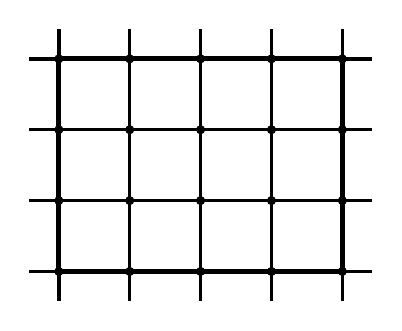
\begin{tikzpicture}[scale=0.75]
  % --- grid size (number of cells) ---
  \def\Nx{4}    % columns of cells
  \def\Ny{3}    % rows of cells
  \def\s{1.2}   % spacing
  \def\ext{0.5}% overshoot amount (in same units as coords)

  % --- draw vertical lines with overshoot ---
  \foreach \i in {0,...,\Nx} {
    \draw[line width=1.2pt]
      (\i*\s,-\ext) -- (\i*\s,\Ny*\s+\ext);
  }

  % --- draw horizontal lines with overshoot ---
  \foreach \j in {0,...,\Ny} {
    \draw[line width=1.2pt]
      (-\ext,\j*\s) -- (\Nx*\s+\ext,\j*\s);
  }

  % --- outer boundary (frame) ---
  \draw[line width=1.8pt] (0,0) rectangle (\Nx*\s,\Ny*\s);

  % --- dots at each intersection (inside the frame) ---
  \foreach \i in {0,...,\Nx} {
    \foreach \j in {0,...,\Ny} {
      \fill (\i*\s,\j*\s) circle (2.2pt);
    }
  }
\end{tikzpicture}
\end{center}

Edges $E$, Vertices $V$, Faces/Plaquette $F/P$;
The qubits be on edges. \\
Periodic boundary conditions = toric code \\
Planar = surface code \\
The goal of all of these constructions is to find a way to represent a stabilizer state, meaning we can write down a series of stabilizer generators which all commute with each other. (This is the fun game with simple rules - just find a systematic way of getting a bunch of stuff commuting and we get a code.) \\

The state generator which will be the products around the edges corresponds to the vertex $v$
\begin{equation}
    A_v = \prod_{e \sim v} X_e \text{ and } B_p =  \prod_{e \sim f} Z_e
\end{equation}

\begin{center}
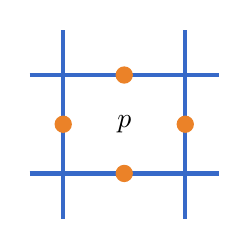
\begin{tikzpicture}[scale=0.5]
  % colors close to the figure
  \definecolor{lineblue}{RGB}{55,105,200}
  \definecolor{dotorange}{RGB}{235,130,40}

  % parameters
  \def\L{2.4}     % half-length of each long line segment
  \def\xs{1.55}   % x-position of the two vertical grid lines
  \def\ys{1.25}   % y-position of the two horizontal grid lines
  \def\r{0.22}    % dot radius

  % grid lines (2 vertical + 2 horizontal)
  \draw[line width=1.5pt, lineblue] (-\xs,-\L) -- (-\xs,\L);
  \draw[line width=1.5pt, lineblue] ( \xs,-\L) -- ( \xs,\L);
  \draw[line width=1.5pt, lineblue] (-\L,-\ys) -- (\L,-\ys);
  \draw[line width=1.5pt, lineblue] (-\L, \ys) -- (\L, \ys);

  % dots (midpoints of each side of the central square)
  \fill[dotorange, line width=1.5pt] (0, \ys)  circle (\r);   % top
  \fill[dotorange, line width=1.5pt] (0,-\ys)  circle (\r);   % bottom
  \fill[dotorange,  line width=1.5pt] (-\xs,0)  circle (\r);   % left
  \fill[dotorange, line width=1.5pt] ( \xs,0)  circle (\r);   % right

  % label
  \node at (0,0) {$p$};
\end{tikzpicture}
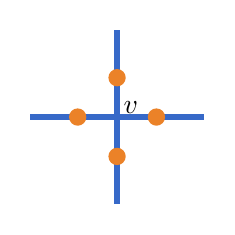
\begin{tikzpicture}[scale=0.5]
  % colors
  \definecolor{lineblue}{RGB}{55,105,200}
  \definecolor{dotorange}{RGB}{235,130,40}

  % parameters
  \def\L{2.2}   % half-length of the cross arms
  \def\r{0.22}  % radius of the dots

  % cross
  \draw[line width=2pt, lineblue] (-\L,0) -- (\L,0);
  \draw[line width=2pt, lineblue] (0,-\L) -- (0,\L);

  % dots (top, bottom, left, right)
  \fill[dotorange,  line width=1.5pt] (0, 1.0) circle (\r);
  \fill[dotorange, line width=1.5pt] (0,-1.0) circle (\r);
  \fill[dotorange, line width=1.5pt] (-1.0,0) circle (\r);
  \fill[dotorange, line width=1.5pt] ( 1.0,0) circle (\r);

  % label
  \node at (0.35,0.25) {$v$};
\end{tikzpicture}
\end{center}

%%%%% Module 2 %%%%% 
%%%%% Week 4 %%%%% 
\section{Lecture 6: Quantum Signal Processing}
Lecture overview:
\begin{enumerate}[label=(\Roman*)]
    \item Conceptual Overview
    \item Quantum signal processing
    \item Eigenvalue transformation
    \item Quantum Singular Value Transformation
\end{enumerate}

\subsection{Conceptual overview}
Quantum signal processing and the quantum singular value transform algorithm capture the essence behind, and fully reproduce (and in some cases improve upon) Grover's quantum search algorithm, the HHL quantum linear systems algorithm, Hamiltonian simulation, quantum phase estimation, and many other algorithms. This works based on two ingredients
\begin{itemize}
    \item block-encoded operator
    \item polynomial transform of its singular values
\end{itemize}

A general unitary transform on $n$ qubits is described by a $2^n \times 2^n$ matrix. The idea of \textit{block encoding} is to use just a sub-block $A$,  of this matrix, which we may take wlog to be the top left block:
\begin{equation}
    \begin{pmatrix}
        A & \ldots \\
        \vdots & \ddots
    \end{pmatrix}
\end{equation}
where the $\norm{A} < 1$ for $U$ to be unitary. In particular the norm of $A$ must be sufficiently small. The dimension of $A$ just needs to be smaller than that of $U$. For example, we may have $A$ being $2^{n-1} \times 2^{n-1}$, such that $A$ inhabits one quarter of the matrix $U$. This example represents the case when one of the $n$ qubits is special, drawn here as a circuit representation of $U$ with the top qubit being separated from the remaining $n - 1$ qubits:




\begin{claim}
    Quantum singular value transformation (informal) \\
    Given $U$ encoding $A$, one can systematically construct a new unitary $U'$ which block encodes $\text{poly}_d^{\text{SV}}(A)$, where in terms of the singular value decomposition of $A$:
    \begin{equation}
        A = \sum_\lambda \lambda \ketbra{v_\lambda}{w_\lambda}
    \end{equation}
    the polynomial is defined as 
    \begin{equation}\poly_d^{\text{SV}}(A) = \sum_\lambda \poly_d(\lambda)\ketbra{v_\lambda}{w_\lambda}\end{equation}
    and $d$ is the degree of the polynomial. This requires $O(d)$ gates and accesses to $U$. Note that only $\sim d$ gates and accesses are required for a degree $d$ polynomial, independent of the size of $A$.
\end{claim}

Quantum algorithms can be mapped onto quantum singular value transformation and vice versa, based on choices for just two ingredients:
\begin{itemize}
    \item The block-encoded operator $A$ - this may be the Hamiltonian we want to simulate, or the matrix we want to invert, or an oracle capturing the search problem
    \item The degree $d$ polynomial designed for the task
\end{itemize}
Quantum signal processing is the method by which a quantum circuit is specified to realize a desired polynomial transformation, and it will be seen that this can be accomplished efficiently. QSVT encompasses the general method of transforming arbitrary implicitly encoded $A$.

\subsection{Quantum Signal Processing}
Consider a single qubit system undergoing the dynamics described \\
\begin{center}
\begin{quantikz}
     & \gate{\phi_{d}} & \gate{R_x(\theta)} & \gate{\phi_{d - 1}} & \gate{R_x(\theta)} & \ \ldots \  & \gate{R_x(\theta)} & \gate{\phi_{0}} & 
\end{quantikz}
\end{center}
where $\phi_k$ is a phase rotation (about $\hat{z}$) by angle $\phi_k$
\begin{equation}
    \begin{quantikz}
        & \gate{\phi_k} & 
    \end{quantikz} = e^{i \phi_k Z}
\end{equation}
and $R_x(\theta)$ is the usual single qubit rotation by angle $\theta$ about $\hat{x}$
\begin{equation}
    \begin{quantikz}
        & \gate{R_x(\theta)} & 
    \end{quantikz} = e^{i \phi_k X/2} = \begin{pmatrix}
        \cos \frac{\theta}{2} & -i \sin \frac{\theta}{2} \\
        -i \sin \frac{\theta}{2} & \cos \frac{\theta}{2}
    \end{pmatrix}
\end{equation}

Let $U_{\vec{\phi}, \theta}$ be the unitary described by circuit. This circuit has $d+1$ phase rotations, and $d$ queries to $R_x(\theta)$. Let
\begin{align}
    a = \cos \left(- \frac{\theta}{2}\right) \\
    \sqrt{1-a^2} = \sin \left(- \frac{\theta}{2}\right)
\end{align}
where $a$ is a real number in the interval $[-1,1]$, such that we may write
\begin{equation}
    W(a) = \begin{pmatrix}
        a & i \sqrt{1-a^2} \\ 
        i\sqrt{1-a^2} & a
     \end{pmatrix} = R_x(-2\cos^{-1}a)
\end{equation}
The parameter $a$ (or equivalently $\theta$) is the input signal, and $R_x(\theta)$ is known as the signal operator; these are given to us, and outside of our control. The set of phase
angles $\vec{\phi} = {\phi_k}$ are under our control, and these describe how the signal is processed. \\

The quantum signal processing theorem establishes that:
\begin{theorem}
    For 
    \begin{equation}
        U_{\vec{\phi}} = e^{i \phi_0 Z} \prod_{k=1}^d W(a) e^{i \phi_k Z} = \begin{pmatrix}
            P(a) & iQ(a)\sqrt{1-a^2} \\ iQ^*(a)\sqrt{1-a^2} & P^*(a)
        \end{pmatrix}
    \end{equation}
    where $P$ and $Q$ are complex polynomials such that 
    \begin{itemize}
        \item $\deg(P) \leq d$ and $\deg(Q) \leq d-1$
        \item $P$ has parity $d \!\mod 2$ and $Q$ has parity $(d-1) \!\mod 2$
        \item $\abs{P}^2 + (1-a^2) \abs{Q}^2 = 1$
    \end{itemize}
    and moreover, any polynomials $P$, $Q$ satisfying these constraints can be realized by some choice of the phase angles $\vec{\phi}$
\end{theorem}



\subsection{Eigenvalue transformation}
Perhaps the most powerful aspect of quantum signal processing and quantum singular value transformations is that the signal a need not be a classical variable of unknown value, but instead, it may be a quantum variable, potentially in superposition. This is illustrated by the quantum eigenvalue transformation algorithm. Suppose we have a signal unitary on $n + 1$ qubits which may be expressed as
\begin{equation}
    U = \begin{pmatrix}
        H & \sqrt{1-H^2} \\
        \sqrt{1-H^2} & -H
    \end{pmatrix}
\end{equation}
where $H$ is some Hermitian matrix, and for $H$ expressed in its eigenbasis:
\begin{equation}
    H = \sum_\lambda \lambda \ketbra{v_\lambda}
\end{equation}


\subsection{Quantum singular value transformation}




\section{Lecture 7: Fourier Transforms and Lattices - 2 March 2026}
Outline: 
\begin{enumerate}[label=(\Roman*)]
    \item The Fourier transform and its Applications to Dirac Combs
    \item Quantum Fourier Transforms
    \item Oracle period finding (1-Dim)
    \item Oracle period finding (k-Dim)
\end{enumerate}

\subsection{The Continuous and Discrete Fourier Transforms and its Applications to Dirac Combs}
\subsubsection{Continuous Fourier Transform}
consider the Fourier transform. The key theme throughout is:
Period in one only because they listing one domain becomes spacing in the dual domain, and spatial shift becomes phase. 


\section{Problem Set 4 - 8 March 2026}
\subsection{QSP Example: BB1}
In Quantum Signal Processing (QSP), we transform a given $x$-rotation "signal operator" $R_x(\theta)$ by interleaving $z$-rotation "signal processing operators" with repetitions of the signal operator. This gives the QSP sequence unitary operator $U_\Phi(\theta) \in SU(2)$:

\subsubsection{Quantum circuit for BB1 as QSP}
This is the BB1 pulse sequence, expressed as a QSP quantum circuit (with time going from left to right, as usual):
\begin{quantikz}[row sep={0.8cm,between origins}, wire types={q,n}]
& \gate{U_x}
& \gate{e^{-i\phi Z}}
& \gate{U_x}
& \gate{e^{2i\phi Z}}
& \gate{U_x}
& \gate{e^{i0 Z}}
& \gate{U_x}
& \gate{e^{-2i\phi Z}}
& \gate{U_x}
& \gate{e^{i\phi Z}}
& \qw \\
& \push{Unknown}
& \push{known}
& \push{Unknown}
& \push{known}
& \push{Unknown}
& \push{known}
& \push{Unknown}
& \push{known}
& \push{Unknown}
& \push{known}
&
\end{quantikz}\\

where $U_x = R_x(\theta)$ and $R_z(\phi) = e^{-i\phi Z / 2}$. Note that $\theta$ is generally unknown, whereas all the $\phi_k$ are known. 

Implement this single-qubit quantum circuit in pytket:
\begin{lstlisting}
    import pytket
    import numpy as np
    
    def bb1_circuit(theta):
        circ = pytket.Circuit(1)        # pytket one-qubit circuit
        phi = np.arccos(-1/4)/2         # BB1 phase angle
        theta = theta / np.pi           # pytket angles have units of pi
        phi = phi / np.pi
    
        # BB1 pulse sequence
        circ.Rx(theta, 0)
        # complete the BB1 pulse sequence here ** CHANGE ME **    
        circ.Rz(2*phi,0)
        circ.Rx(theta, 0)
        circ.Rz(-4*phi,0)
        circ.Rx(theta, 0)
        circ.Rz(0,0)
        circ.Rx(theta, 0)
        circ.Rz(4*phi,0)
        circ.Rx(theta, 0)
        circ.Rz(-2*phi,0)
        
        return(circ)

\end{lstlisting}


\subsubsection{BB1 response function}
Consider the response $p(\theta) = \braket{0|U|0}$ for $U = R_x(\theta)$ being a single rotation pulse, versus $U = U_\Phi$  being the BB1 pulse sequence. Plotting $p(\theta)$ versus $\theta$ gives, for the two cases:\\

Expand $p$ as a power series in $\theta$ around $\theta=0$, to give:
\begin{equation}
    p = 1 + c \theta^k + O(\theta^{k+1})
\end{equation}
such that 
\begin{itemize}
    \item $k$ represents the order of the first non-vanishing error term (indicating how "flat" the response is).
    \item $c$ is the numerical coefficient of that leading error term.
\end{itemize}


Using the code below to evaluate $p(\theta) = \braket{0|U|0}$,
\begin{lstlisting}
    from pytket.utils.symbolic import circuit_to_symbolic_unitary

    theta = sympy.Symbol("theta")
    bc = bb1_circuit(theta)
    symu = circuit_to_symbolic_unitary(bc)
    p = symu[0,0]
    p = sympy.simplify(p)
    print(p)
    
    def chop_small(expr, threshold=1e-10):
        """Replaces any float smaller than threshold with 0."""
        return expr.xreplace({n: 0 for n in expr.atoms(sympy.Float) if abs(n) < threshold})
    
    chop_small(p.series(theta,0, 8).evalf(chop=True))
\end{lstlisting}

\noindent\fbox{%
  \parbox{\dimexpr\linewidth-2\fboxsep-2\fboxrule}{%
    From the code above, the output is:
    \begin{align}
        &((1.875 + 0.484122918275927i)*\sin(0.159154943091896\pi\theta)^4 + \cos(0.159154943091896\pi\theta)^4 \notag \\ 
        & \quad - 0.3125\cos(0.636619772367582\pi\theta) + 0.3125)*\cos(0.159154943091896\pi\theta) \\
        & = 1.0 + 0.0302576823922455i\theta^4 + \theta^6(-0.00488281250000001 - 0.00882515736440497i) + O(\theta^8)
    \end{align}
    Therefore $k = 4$ and $c = 0.0302576823922455$
    }%
}
\newpage
\subsection{Problem 2 - The Quantum Fourier Transform (QFT)}
This problem explores the structure of the Quantum Fourier Transform (QFT) and how it can be used to perform state preparation and phase manipulations. You will analyze the effect of applying phase shifts in the Fourier basis.

The Quantum Fourier Transform (QFT) is the "engine" behind Shor’s algorithm and many other quantum speedups. While classically the Discrete Fourier Transform (DFT) on $N$ points takes$O(N\log N)$ time, the QFT on $n$ qubits (where $N = 2^n$) can be performed in $O(n^2)$ gates.

Recall the definition of the QFT acting on a basis state $\ket{j}$ for a system of dimension $N$: 
\begin{equation}
    \mathrm{QFT}_N \ket{j} = \frac{1}{\sqrt{N}} \sum_{k=0}^{N-1}\omega_N^{jk}\ket{k}
\end{equation}
where $\omega_N = e^{2\pi i/N}$ is the $N$-th root of unity.

\subsubsection{QFT on 2 Qubits}
Consider a 2-qubit system ($N=4$). We apply the QFT to the state $\ket{1}$ (which is $\ket{01}$ in binary.\\

After apply $\mathrm{QFT}_4$ to the state $\ket{1}$, the result state is $\frac{1}{2} \sum_{k=0}^3 \alpha_k \ket{k}$. What is the value of the coefficient $\alpha_2$? 

\noindent\fbox{%
  \parbox{\dimexpr\linewidth-2\fboxsep-2\fboxrule}{%
        \begin{align}
            \mathrm{QFT}_4 \ket{1} &= \frac{1}{2} \sum_{k=0}^3 \alpha_k \ket{k} \\
            &=  \frac{1}{\sqrt{N}} \sum_{k=0}^{N-1}\omega_N^{jk}\ket{k} \\
            &= \frac{1}{2} \left[e^{2\pi i 1\cdot 0/4}\ket{0} + e^{2\pi i 1\cdot 1/4}\ket{1} + e^{2\pi i 1\cdot 2/4}\ket{2} + e^{2\pi i 1\cdot 3/4}\ket{3}\right]
        \end{align}
        From here we can read off the coefficient $\alpha_2 =  e^{2\pi i 1\cdot 2/4} = e^{i \pi} = -1$. 
    }%
}
\subsubsection{Visualizing the Phase}
The QFT can be viewed as "encoding" the value $j$ into the phases of a uniform superposition. \\

If we apply the QFT to a basis state $\ket{j}$ and get some state $\sum_k c_k\ket{k}$, what is the relative phase between $c_k$ and $c_{k+1}$, namely $\Delta = c_{k+1}^*c_k$? 

\noindent\fbox{%
    \parbox{\dimexpr\linewidth-2\fboxsep-2\fboxrule}{%
        \begin{align}
            \Delta &= c_{k+1}^*c_k \\
            &= \frac{1}{\sqrt{N}} (e^{2\pi i j(k+1)/N})^*\frac{1}{\sqrt{N}}(e^{2\pi i j k/N}) \\
            &= \frac{1}{N}(e^{- 2\pi i j(k+1)/N})(e^{2\pi i j k/N}) \\
            &= \frac{1}{N}\exp[2\pi i j/N (-k-1 + k)] \\
            &= \frac{1}{N}\exp[-2\pi i j/N]
        \end{align}
    }%
}




\subsubsection{The Inverse QFT and Pattern Recognition}
In period finding, we usually end up with a periodic state in the computational basis and apply the Inverse QFT ($\mathrm{QFT}^\dagger$) to extract the period. \\

Suppose $N=8$, ($3$ qubits). We have a state that is a uniform superposition of all even basis states:
\begin{equation}
    \ket{\psi} = \frac{1}{2} (\ket{0} + \ket{2} + \ket{4} + \ket{6})
\end{equation}

This state has a period $T = 2$. If we apply $\mathrm{QFT}_8$ to the state $\ket{\psi}$ defined above,which basis states will have non-zero probability of being measured? \\

\noindent\fbox{%
  \parbox{\dimexpr\linewidth-2\fboxsep-2\fboxrule}{%
The QFT is defined as 
\begin{equation}
    \mathrm{QFT}_N \ket{j} = \frac{1}{\sqrt{N}} \sum_{k=0}^{N-1}\omega_N^{jk}\ket{k}
\end{equation}
where $\omega_N = e^{2\pi i/N}$ is the $N$-th root of unity.

\begin{align}
    \mathrm{QFT}_8 \ket{\psi} &=\mathrm{QFT}_8\left[\frac{1}{2} (\ket{0} + \ket{2} + \ket{4} + \ket{6})\right] \\
    &= \frac{1}{4}\left[\left(\sum_{k=0}^7\omega_8^{0k} \ket{k}\right) + \left(\sum_{k=0}^7\omega_8^{2k} \ket{k}\right) + \left(\sum_{k=0}^7\omega_8^{4k} \ket{k}\right) + \left(\sum_{k=0}^7\omega_8^{6k} \ket{k}\right) \right] \\
    &= \frac{1}{4}\left[\sum_{k=0}^7\left(\omega_8^{0k} + \omega_8^{2k} + \omega_8^{4k} + \omega_8^{6k}\right)\ket{k}\right] \\
    &= \frac{1}{4}\left[\sum_{k=0}^7\left(e^{2\pi i 0\cdot k/8} + e^{2\pi i 2\cdot k/8} + e^{2\pi i 4\cdot k/8} + e^{2\pi i 6\cdot k/8}\right)\ket{k}\right] \\
    &= \frac{1}{4}\left[\sum_{k=0}^7\left(1 + e^{2\pi i 2\cdot k/8} + e^{2\pi i 4\cdot k/8} + e^{2\pi i 6\cdot k/8}\right)\ket{k}\right] \\
    &= \frac{1}{4}\left[\left(1 + e^{2\pi i 2\cdot 0/8} + e^{2\pi i 4\cdot 0/8} + e^{2\pi i 6\cdot 0/8}\right)\ket{0} + \left(1 + e^{2\pi i 2\cdot 1/8} + e^{2\pi i 4\cdot 1/8} + e^{2\pi i 6\cdot 1/8}\right)\ket{1}\right. \notag \\
    &\qquad + \left(1 + e^{2\pi i 2\cdot 2/8} + e^{2\pi i 4\cdot 2/8} + e^{2\pi i 6\cdot 2/8}\right)\ket{2} + \left(1 + e^{2\pi i 2\cdot 3/8} + e^{2\pi i 4\cdot 3/8} + e^{2\pi i 6\cdot 3/8}\right)\ket{3} \notag \\
    &\qquad + \left(1 + e^{2\pi i 2\cdot 4/8} + e^{2\pi i 4\cdot 4/8} + e^{2\pi i 6\cdot 4/8}\right)\ket{4} + \left(1 + e^{2\pi i 2\cdot 5/8} + e^{2\pi i 4\cdot 5/8} + e^{2\pi i 6\cdot 5/8}\right)\ket{5} \notag \\
    &\left.\qquad + \left(1 + e^{2\pi i 2\cdot 6/8} + e^{2\pi i 4\cdot 6/8} + e^{2\pi i 6\cdot 6/8}\right)\ket{6} + \left(1 + e^{2\pi i 2\cdot 7/8} + e^{2\pi i 4\cdot 7/8} + e^{2\pi i 6\cdot 7/8}\right)\ket{7} \right] \\
    &= \frac{1}{4}\left[\left(1 + 1 + 1 + 1\right)\ket{0} + \left(1 + e^{\pi i /2} - 1 + e^{12\pi i/8}\right)\ket{1} + \left(1 -1 + 1 + -1\right)\ket{2} + \left(1 + e^{12\pi i /8} - 1 + e^{32\pi i /8}\right)\ket{3} \right. \notag \\
    &\qquad\left. + \left(1 + 1 + 1 + 1\right)\ket{4} + \left(1 + e^{20\pi i /8} - 1 + e^{60\pi i /8}\right)\ket{5} + \left(1 -1 -1 + 1\right)\ket{6} + \left(1 + e^{28\pi i /8} -1 + e^{84\pi i /8}\right)\ket{7}\right]
\end{align}
We want to know which states will have non-zero probability of being measured. If we do 
\begin{equation}
    \norm{\braket{\psi|\mathrm{QFT}_8^\dagger \mathrm{QFT}_8| \psi}}^2
\end{equation}
we can only see that the $\ket{0}$ and $\ket{4}$ terms survive. 
}%
}

\subsubsection{Constructive Interference}
The reason we only see certain values is due to constructive interference. For a state with period $T$, the QFT concentrates the amplitude on multiples of $N/T$.\\

Suppose $N = 1024$ and we have a periodic state with period $T=16$. If we measure the state after a QFT, what is the smallest non-zero integer we are likely to observe? \\
\noindent\fbox{%
  \parbox{\dimexpr\linewidth-2\fboxsep-2\fboxrule}{%
\begin{equation}
    \frac{N}{T} = \frac{1024}{16} = 64
\end{equation}
}%
}

\subsubsection{Phase Rotations in the Fourier Basis}
Consider the following operation sequence $U$:
\begin{enumerate}
    \item Apply $\mathrm{QFT}_N$.
    \item Apply a phase gate $\exp(2\pi i \alpha Z)$ to each qubit
    \item Apply $\mathrm{QFT}^\dagger_N$.
\end{enumerate}
If we apply $U$ to the state $\ket{x}$, what is the resulting state $\ket{v} = U\ket{x}$. \\

\noindent\fbox{%
  \parbox{\dimexpr\linewidth-2\fboxsep-2\fboxrule}{%
The following operation can be described as the following
\begin{equation}
    U = \mathrm{QFT}_N^\dagger e^{2\pi i \alpha Z}\mathrm{QFT}_N 
\end{equation}
We know that 
\begin{equation}
    \mathrm{QFT}_N\ket{x} = \frac{1}{\sqrt{N}}\sum_{y=0}^{N-1} e^{2\pi i xy/N}\ket{y}
\end{equation}

\begin{align}
    e^{2 \pi i \alpha Z} &= \cos(2\pi \alpha) I + i \sin(2\pi \alpha) Z \\
    &= \begin{pmatrix}
        \cos(2\pi \alpha) + i \sin(2\pi \alpha) & 0 \\
        0 & \cos(2\pi \alpha) - \sin(2\pi \alpha)
    \end{pmatrix} \\
    &= \begin{pmatrix}
        e^{2\pi i \alpha} & 0 \\
        0 & e^{-2\pi i \alpha}
    \end{pmatrix}
\end{align}


Then the resulting state $\ket{v}$ is 
\begin{align}
    \ket{v} &= U\ket{x} \\
    &= \mathrm{QFT}_N^\dagger e^{2\pi i \alpha Z}\mathrm{QFT}_N \ket{x} \\
    &= \frac{1}{\sqrt{N}} \mathrm{QFT}_N^\dagger e^{2\pi i \alpha Z} \sum_{y=0}^{N-1} e^{2\pi i xy / N}\ket{y} \\
    &= \frac{1}{\sqrt{N}} \mathrm{QFT}_N^\dagger \sum_{y=0}^{N-1} e^{2\pi i xy / N}e^{2\pi i \alpha y}\ket{y} \\
    &= \frac{1}{\sqrt{N}} \mathrm{QFT}_N^\dagger \sum_{y=0}^{N-1} e^{2\pi i (x + \alpha N)y / N}\ket{y} \\
    &= \mathrm{QFT}_N^\dagger \mathrm{QFT}_N \ket{x + \alpha N} \\
    &= \ket{x + \alpha N} \\
\end{align}
}%
}

\newpage
\subsection{Problem 3 - Jevons' constant}
In 1874, the English economist William Stanley Jevons wrote in his work Principles of Science:\\
Can the reader say what two numbers multiplied together will produce the number 8,616,460,799? I think it unlikely that anyone but myself will ever know.\\

Use sympy to find the factors of this number.
\begin{lstlisting}
    import sympy

    def factor():
        N = 8616460799
        # write code here to get p and q such that p * q = N
        prime_factors_list = sympy.primefactors(N)
        p=prime_factors_list[0]
        q=prime_factors_list[1]
        return p, q

\end{lstlisting}


\newpage
\subsection{Problem 4 - Factoring larger integers}
We will need to go a lot bigger than Jevons' number if we want factoring to be hard. It turns out making $N$ bigger is necessary, but not sufficient, for factoring to be hard! Indeed, certain special-purpose factoring algorithms make certain numbers surprisingly easy to factor. \\

Play around with the following code using the accompanying colab notebook to get a sense of what makes a number easy or hard to factor. Note that sympy tries several different factoring algorithms under the hood, in order to exploit different properties that might make a number easy to factor.\\ 

\begin{lstlisting}
    def generate_composite(factor_bit_lengths):
    	"""
    	Generate a random composite number N, whose factors have the bit lengths
    	given in the list factor_bit_lengths.
    	"""
    	rtn = 1
    	for nbits in factor_bit_lengths:
    		rtn *= sympy.randprime(2**(nbits-1), 2**nbits)
    	return rtn
      
    N = generate_composite([64, 64])
    factor(N)
\end{lstlisting}

Answer the this multiple-choice question with the understanding that:
\begin{itemize}
    \item ``Completely factor" means find \textit{all} prime factors
    \item  a ``$k$-bit number" $x$ means $2^{k-1}\leq x < 2^k$
    \item For the purposes of this question, ``quickly" means ``can be completed on a laptop in under a minute". In the question below, none of the options are ``borderline"; they are either much cheaper than 1 minute on a laptop, or much more expensive.
\end{itemize}

Note: sympy's factoring function with default settings will not quickly succeed on all of the "true" options below. Sometimes it gets "stuck" trying a factoring algorithm that is not appropriate for the given number. Here are some things to look at for the trickier ones:
\begin{itemize}
    \item Sympy's documentation of the elliptic curve method
    \item Fermat's factorization method (see in particular the paragraph at the end of the "basic method" section)
    \item Sympy's integernthroot function
\end{itemize}


Mark the completions that make the following statement true: ``A number $N$ can typically be completely factored quickly if, \\
\noindent\fbox{%
  \parbox{\dimexpr\linewidth-2\fboxsep-2\fboxrule}{%
\begin{itemize}
    \item it has two independently random 1024-bit prime factors - FALSE
    \item it has 64 independently random 32-bit prime factors - TRUE (? but I let this run for 15 minutes on my Colab)
    \item it has 6 independently random prime factors with bit lengths 8, 16, 24, 32, 512, and 1024 - FALSE
    \item it has 6 independently random prime factors with bit lengths 8, 16, 24, 32, 48, and 1024 - TRUE
    \item it has two 1024-bit prime factors $p$ and $q$ such that $\abs{p-q} < 2^{256}$ - TRUE
    \item it is of the form $N=p^k$, generated by taking a random 1024-bit prime $p$ and raising it to a random integer $k$ - TRUE
    \item it is a random 2048-bit integer - FALSE
    \item it is a 2048-bit prime (i.e. can it be shown to be prime itself?) - TRUE
\end{itemize}
}%
}

\newpage
\subsection{Problem 5 - Factoring via greatest common divisor (GCD)}
The following two 2048-bit integers are of the form $N=pq$ and $M=p'q$, where $p,p',q$ are independently chosen random 1024-bit prime numbers. That is, they each have two factors, but share exactly one of those factors. \\

Completely factor both of the following integers:
\begin{align}
    N &= 159561411736037650842019124481796807324653887498957019629693014541934972183567204227090048408510 \notag \\
    &0594623667305823548069239886835926577827307963162794252537977761232853616531034623384624193949447948 \notag \\
    &2729739717981515034610081599748088566170735181775069833678327297641125301847641581785458916257668327 \notag \\
    &1496994091982625236831691115784289288601428297252619706889242210655171991531524434059614632842548539 \notag \\
    &2085388716024207148066709346005591720423815927809654581005922834289243666711697761849453572709254404 \notag \\
    &2008680162164394618561967958640596584574851594992002821134408274551341181004283029878977210398250107 \notag \\
    &932326435166672158783 \\
    M &= 197522169540569518410872161674921093361642926577863700550819484785864780322285005242395528760276 \notag \\
    &2513020211613081148242140775277536585325936056579361506718814695400934698319342664131435070116939766 \notag \\
    &4979533865953115520677515139471918301325427435066428085291947839137221435063741367676152991685877443 \notag \\
    &2231453177697795313922894454281778061507602728517409577605989931930702324895943430604183916347145650 \notag \\
    &8984034021008099278125019917820630490974999306015737191466142018044916599340159431249755004434587385 \notag \\
    &4706062818840944811973901557690394700783290278061812190021681573748368419641902330577496400417103902 \notag \\
    &974764441598764147391
\end{align}


\begin{lstlisting}
    N = (number in (12.27))
    M = (number in (12.28))

    
    p = sympy.gcd(N,M)
    print(f"p={p}")
    
    q1 = N//p
    q2 = M//p
    print(f"q1 = N/p={N/p}")
    print(f"q2 = M/p={M/p}")
    assert(q1 * p == N)
    assert(q2 * p == M)
\end{lstlisting}

\noindent\fbox{%
  \parbox{\dimexpr\linewidth-2\fboxsep-2\fboxrule}{%
1434479188310610121491452576747852241279360893200798140186898204494123419282799437437880665917483
2788856336366905219768190021301778280400637439599169562422453076700890524978061539130492082832709
2665394992044261829429798263455243699549745801990350836742392901838631978262884860079993111405104
624378572690015873
}%
}\\

This can actually be a serious problem in computer security: if you use a faulty random number generator to generate the primes $p$ and $q$  for cryptographic purposes, it might turn out that one of them is not particularly random at all. If you can find two cryptographic keys $M$ and $N$ that share exactly one factor, you can break both of them! See for example: Heninger et al., ``Mining Your Ps and Qs: Detection of Widespread Weak Keys in Network Devices".


\newpage
\subsection{A quantum algorithm for discrete logarithms}
For any integer $M$, the nonnegative integers $a<M$ that are co-prime to $M$ form a group under multiplication $\mod M$. This group can be denoted $\mathbb{Z}^*_M$. \\

The discrete logarithm problem over integers $\mod M$ is thus defined as follows:
\begin{definition}
    Given an integer $M$, and integers $g, w \in \mathbb{Z}^*_M$, find an integer $s$ such that $g^* \equiv w (\mod M)$ (given the promise that such an $s$ exists).
\end{definition}

With appropriate parameters, this problem is computationally hard classically, and is the basis of a wide array of cryptosystems, most importantly Diffie-Hellman key exchange and the Digital Signature Algorithm (DSA).

In quantum computing, Shor's algorithm for discrete logarithms relies on the fact that we can find the "period" of a function in a high-dimensional space. Let's explore the math behind this classically using a small prime-order subgroup of $\mathbb{Z}^*_M$.

Consider the group $\mathbb{Z}^*_{23}$ (integers modulo 23 under multiplication). Let $g=2$ be a generator for a subgroup.

\subsubsection{Group Order}
First, we want to determine the order $p$ of the subgroup generated by $g$. Find the smallest integer $p > 0$ such that $g^p \equiv 1\mod{23}$

\noindent\fbox{%
  \parbox{\dimexpr\linewidth-2\fboxsep-2\fboxrule}{%
\begin{align}
    2^1 &= 2 \\
    2^2 &= 4 \\
    2^3 &= 8 \\
    2^4 &= 16 \\
    2^5 &= 32 - 23 = 9\\
    2^6 &= 64 -(2\cdot23) = 18 \\
    2^7 &= 128 -(5\cdot23) = 13 \\
    2^8 &= 256 - (11\cdot23) = 3 \\
    2^9 &= 512-(22\cdot23) = 6 \\
    2^{10} &= 1024-(44\cdot23) = 12 \\
    2^{11} &= 2048-(89\cdot23) = 1 \\
\end{align}
Therefore, the smallest integer $p>0$ such that $g^p \equiv 1\mod{23}$ is $p=11$.
}%
}

\subsubsection{The Discrete Logarithm}
Now, suppose we are given the value $w=18$. Because $p$ is prime, we are guaranteed that $w$ exists within the subgroup $\langle g\rangle$. Find the discrete logarithm $s$ such that $g^p \pmod 1 \mod 23$\\
\noindent\fbox{%
  \parbox{\dimexpr\linewidth-2\fboxsep-2\fboxrule}{%
From the previous question we saw that $2^6 = 64 -(2\cdot23) = 18$, therefore, $s=6$
}%
}


\subsubsection{A periodic function for discrete log: numerical example}
Consider the function
\begin{equation}
    f(x,y) = g^x \cdot w^{-y} \mod{23}
\end{equation}
and note that the modular inverse $18^{-1} \mod{23}=9$\\
Compute the value of $f(1,1)$\\
\noindent\fbox{%
  \parbox{\dimexpr\linewidth-2\fboxsep-2\fboxrule}{%
\begin{align}
    f(1,1) &= 2^1\cdot 18^{-1} \mod 23 \\
    &=2 \cdot 9 \mod 23 \\
    &= 18 \mod 23
\end{align}
}%
} \\\\
Compute the value of $f(1+s,2)$ using the $s$ you found above\\
\noindent\fbox{%
  \parbox{\dimexpr\linewidth-2\fboxsep-2\fboxrule}{%
\begin{align}
    f(1+6,2) &= 2^7\cdot 18^{-1}\cdot 18^{-1} \mod 23 \\
    &=13 \cdot 81 \mod 23 \\
    &= 18 \mod 23
\end{align}
}%
} 

\newpage
\subsection{Quantum period finding for the discrete logarithm problem}
Following what we've learned in class, let's apply quantum period finding to solve the discrete logarithm problem. The first step is to find a periodic function whose period gives us information about the value $s$ we are trying to compute. Then we can apply quantum period finding to extract that period.

\subsubsection{A periodic function for discrete log}
For the purposes of this problem, let's assume that $g$ generates a prime-order subgroup of $\mathbb{Z}^*_M$, and furthermore that we know the order $p$. Put another way: suppose that along with $M$ and $g$, we are handed a prime $p$ for which $g^p \equiv 1 \mod M$.

To factor an integer $N$, we perform period finding on the function $f(x) = a^x \mod N$, and this gives us the order of the group generated by $a$. It might feel intuitive that for discrete log we should try finding the order of $f(x) = w^x \mod M$. Would this help us find $s$ such that $w = g^s \mod M$?  \\

Let's approach this systematically. First, what is the period of the function $f(x) = w^x \mod M$. \\

\noindent\fbox{%
  \parbox{\dimexpr\linewidth-2\fboxsep-2\fboxrule}{%
The period of the function $f(x) = w^x \mod M$ is the order, and we were given $M, g,$ and a prime $p$ for which $g^p \equiv 1 \mod M$. Therefore, the period $= p$. 
}%
} \\\\


Well, that's not helpful: we already knew that! Let's try again. Consider the following function:
\begin{equation}
    f(x_0,x_1) = g^{x_0}w^{x_1} \mod M
\end{equation}
Note this function has two inputs, so the period should be of the form $\vec{T} = (T_0,T_1)$. It should hold that $f(x_0',x_1') = f(x_0,x_1)$ if and only if there exists an integer $j$ such that $\vec{x}' = \vec{x} + j \vec{T} \mod p$. (with all arithmetic done $\mod p$). Give $T_0$ and $T_1$ in terms of the known variables in this problem.

\noindent\fbox{%
  \parbox{\dimexpr\linewidth-2\fboxsep-2\fboxrule}{%
\begin{align}
    f(x_0,x_1) &= g^{x_0}w^{x_1} \mod M \\
    &= g^{x_0} g^{sx_1} \mod M \\
    f(x_0,x_1) &= g^{x_0 + sx_1} \mod M
\end{align}
It should hold that $f(x_0',x_1') = f(x_0,x_1)$ if and only if there exists an integer $j$ such that $\vec{x}' = \vec{x} + j \vec{T} \mod p$, therefore 
\begin{equation}
    f(x_0',x_1') = f(x_0+jT_0, x_1+jT_1) = f(x_0,x_1)
\end{equation}
Then, 
\begin{equation}
    f(x_0 + jT_0, x_1 + jT_1) = g^{x_0+jT_0 + s(x_1 + jT_1)} \mod M
\end{equation}
and we must have that 
\begin{align}
    jT_0 + sjT_1 = 0
\end{align}
Therefore, we can choose $T_0 = -s$, and $T_1 = 1$.
}%
}

\subsubsection{Dual lattice}
In a moment we will go through all the machinery of writing down the quantum states at each step of period finding, taking their Fourier transforms, etc. But first we get to see the power of lattices, that allows us to skip all of that. \\

We learned in lecture that when we take the Fourier transform along each dimension of the multidimensional "comb state" with period $\vec{T}$, we get out a superposition over all vectors having $\vec{y} \cdot \vec{T} = 0 \mod p$. In terms of lattices, this corresponds to the dual lattice, which is the all of the vectors orthogonal to the primal (coset) lattice corresponding to the original comb state. \\

We want to find $\vec{y} = (y_0, y_1)$ of the new comb state after the QFT---or equivalently, a basis vector for the dual lattice---written in terms of $s$. Subjectively, this should be the "simplest" possible $\vec{y} = (y_0, y_1)$ such that $\vec{y} \cdot \vec{T} = 0 \mod p$. \\

\noindent\fbox{%
  \parbox{\dimexpr\linewidth-2\fboxsep-2\fboxrule}{%
From above, we saw that $T_0 = -s = p-s$, and $T_1 = 1$. We need 
\begin{equation}
    \vec{y} \cdot \vec{T}  = y_0T_0 + y_1T_1= 0 \mod p
\end{equation}
From here the ``simplest possible $\vec{y} = (y_0,y_1) = (1,s)$
}%
}


\subsubsection{Quantum period finding in 2D}
This suggests that if we go through with quantum period finding, the result we should get out is a random multiple of that. We begin the quantum period finding algorithm by setting up the following state (suppressing normalizations for clarity):
\begin{equation}
    \sum_{x_0}^{p-1}\sum_{x_1}^{p-1} \ket{x_0}\ket{x_1} \ket{g^{x_0}w^{w_1} \mod M }
\end{equation}
As usual, the next step is to measure the ``output register, returning some group element $y$. \\

We have that $y = g^{x_0}w^{x_1}\mod M$. Write this in terms of only $g,s,x_0,x_1,M$. \\

From above we have that $w = g^s \mod M$, so substituting into $y$ gives us
\begin{align}
    y &= g^{x_0}w^{x_1}\mod M \\
    &= g^{x_0}(g^s)^{x_1} \mod M \\
    &= g^{x_0 + sx_1} \mod M
\end{align}
    
Let $c$ be an integer such that $y = g^c$. Dropping the output register we just measured, we now have the following state:
\begin{equation}
    \sum_{x_0,x_1|c=x_0 + sx_1} \ket{x_0}\ket{x_1} = \sum_{x_1=0}^{p-1} \ket{c-sx_1} \ket{x_1}
\end{equation}
for some $c$ (for which $y = g^c$). If we now take the quantum Fourier transform with modulus $p$ of these two registers, we get: 
\begin{equation}
    \sum_{y_0 =0}^{p-1}\sum_{y_1 =0}^{p-1}\sum_{x_0 =0}^{p-1} e^{2\pi i (c-sx_1)y_0/p}e^{2 \pi i x_1 y_1 / p} \ket{y_0} \ket{y_1} = \sum_{y_0,y_1} e^{2 \pi i c/p} \left[\sum_{x_1}e^{2\pi i (y_1 - sy_0)/p}\right] \ket{y_0}\ket{y_1}
\end{equation}
Now for the very important part. Let $a = y_1 - sy_0$, and consider the following question: For any non-zero integer $a$ such that $0 < a < p$, what is the value of 
\begin{equation}
    \sum_{x_1=0}^{p-1} e^{2\pi i x_1 a/ p}
\end{equation}

\noindent\fbox{%
  \parbox{\dimexpr\linewidth-2\fboxsep-2\fboxrule}{%
Using geometric sum, 
\begin{align}
    \sum_{x_1=0}^{p-1} e^{2\pi i x_1 a/ p} & = \frac{1 -e^{2 \pi i a \cdot p/p}}{1 - e^{ 2\pi i a/p}} \\ 
    &= \frac{1 -e^{2 \pi i a }}{1 - e^{ 2\pi i a/p}}
\end{align}
For any integer $0 < a < p$, $e^{2 \pi i a} = 1$, therefore,
\begin{equation}
    \sum_{x_1=0}^{p-1} e^{2\pi i x_1 a/ p}  = 0
\end{equation}
}%
}


\subsubsection{The period!}
This brings us to our big moment: given the above, the only values of $y_0$ and $y_1$ that will have nonzero probability of measurement are those for which $y_1 -sy_0 \equiv 0 \mod p$. \\

If we now measure the registers holding $y_0$ and $y_1$, we are guaranteed to get values for which this relationship holds. Observe that such vectors are all integer multiples of the dual lattice basis vector we found above. \\

Now for the grand finale: solve for $s$ in terms of $y_0$ and $y_1$, using modular inverses if necessary (and assume this is 
$\mod p$). \\

\noindent\fbox{%
  \parbox{\dimexpr\linewidth-2\fboxsep-2\fboxrule}{%
\begin{equation}
    y_1 -sy_0 \equiv 0 \Rightarrow y_1 = sy_0 \Rightarrow s = (y_0)^{-1}y_1
\end{equation}
}%
}



\subsubsection{Real Example}
Suppose this is the following discrete logarithm problem over a multiplicative group of integers:
\begin{align}
    M &= 1095550635930499780328836414265613952331296552518307158401468301279464852292985836534577579704019393 \notag \\
    &06518068610993318061680053829828007817761863357435454036528274297904172133116946345116794394821415178264 \notag \\
    &870822647137796780969201371084096191228398246824739528671084440237463388177371566396396125234680083052107 \\
    \notag \\
    g &= 4 \\
    \notag \\
    w &= 1830104363094415330119253691710843018713108382528896575327557338092803995952710295675988751077307534 \notag \\
    &87434904633278008421545772254490936964505797156644220939497569164732185192675720179206113244515964966306 \notag \\
    &45374422190105536549936395638455664693560182656495650571179357625293599309221766299968467709714744663000
\end{align}
Recall, your goal is to find some $s$ such that $g^s \equiv w \mod M$. Suppose you run the algorithm described above on your quantum computer, and measure the following results: 
\begin{align}
    y_0 &= 897374748569185086389714192807682256550514976884135801112484108919210136525639372079954707785842370 \notag \\
    &15105668869413656454918335423184883171058484429026662448482971813243629924388023455828859083362628888148 \notag \\
    &32481925003108298224703486970428065787835183709493132398177983762839306431729910996023695339441979095905 \\
    \notag \\
    y_1 &= 297449510752121271826654544782620643188195652943251749153605047937416124898828997833139549263153514 \notag \\
    &96123270672401630748583070649867632482902932638378032551865971532525949387085399875497160761163267211080 \notag \\
    &10132429371019393320757153085165452257306397792174570580018051830005321730256083552594060220096339912730 \notag \\
    &65900631124344157646517713197844426347440589103000736208299198184913886573705
\end{align}

Given these values, compute $s$ such that $w = g^s \mod M$:

\noindent\fbox{%
  \parbox{\dimexpr\linewidth-2\fboxsep-2\fboxrule}{%
We need to calculate $s = (y_0)^{-1}y_1$. We first need to find the modular inverse of $y_0$.
\begin{align}
y_0^{-1}= &72500626049479460629106151733487205214100361162073684529569546401215661196 \notag\\
&39830230395008397483541712725094942291828189853231700326656581357397800732 \notag\\
&93948220972881037226508324548420428643185631174267405398570331041328946348 \notag\\
&09805750711806242732366924108836878280492317899301646114709571908750700461 \notag\\
&430115205007
\end{align}
Then,
\begin{equation}
    s=y_0^{-1} y_1 \mod M = 33146632577570099237373573513513327566297498444842356751283756760092278878761
\end{equation}
}%
} \\ \\

Bonus question: convert the integer $s$ into a 32-byte ASCII encoded string: \\
\begin{lstlisting}
    n = 33146632577570099237373573513513327566297498444842356751283756760092278878761
    print(n.to_bytes(32,'big').decode())
\end{lstlisting}

\noindent\fbox{%
  \parbox{\dimexpr\linewidth-2\fboxsep-2\fboxrule}{%
Output of code: IHTFP (I hold the Fourier power). \\
  
Under the hood explanation from ChatGPT: \\
First we convert the number 33146632577570099237373573513513327566297498444842356751283756760092278878761 to hexadecimal (base 16). This gives us 
\begin{equation}
    494854465020284920686f6c642074686520466f757269657220706f77657229
\end{equation}
This is 64 hex digits, therefore this is 32 bytes long. We then group the hex digits into pairs:
\begin{align}
    &49 \ 48 \ 54 \ 46 \ 50 \ 20 \ 28 \ 49 \notag \\
    &20 \ 68 \ 6f \ 6c \ 64 \ 20 \ 74 \ 68 \notag \\
    &65 \ 20 \ 46 \ 6f \ 75 \ 72 \ 69 \ 65 \notag \\
    &72 \ 20 \ 70 \ 6f \ 77 \ 65 \ 72 \ 29 \notag 
\end{align}
Then we convert each byte to ASCII
\begin{table}[h!]
\centering
\begin{tabular}{|c c c|c c c|c c c|c c c|}
\hline
\textbf{Hex} & \textbf{Dec} & \textbf{ASCII} &
\textbf{Hex} & \textbf{Dec} & \textbf{ASCII} &
\textbf{Hex} & \textbf{Dec} & \textbf{ASCII} &
\textbf{Hex} & \textbf{Dec} & \textbf{ASCII} \\
\hline
49 & 73 & \texttt{I} &
20 & 32 & \textvisiblespace &
46 & 70 & \texttt{F} &
70 & 112 & \texttt{p} \\

48 & 72 & \texttt{H} &
68 & 104 & \texttt{h} &
6f & 111 & \texttt{o} &
6f & 111 & \texttt{o} \\

54 & 84 & \texttt{T} &
6f & 111 & \texttt{o} &
75 & 117 & \texttt{u} &
77 & 119 & \texttt{w} \\

46 & 70 & \texttt{F} &
6c & 108 & \texttt{l} &
72 & 114 & \texttt{r} &
65 & 101 & \texttt{e} \\

50 & 80 & \texttt{P} &
64 & 100 & \texttt{d} &
69 & 105 & \texttt{i} &
72 & 114 & \texttt{r} \\

20 & 32 & \textvisiblespace &
20 & 32 & \textvisiblespace &
65 & 101 & \texttt{e} &
29 & 41 & \texttt{)} \\

28 & 40 & \texttt{(} &
74 & 116 & \texttt{t} &
72 & 114 & \texttt{r} &
 &  &  \\

49 & 73 & \texttt{I} &
68 & 104 & \texttt{h} &
20 & 32 & \textvisiblespace &
 &  &  \\
\hline
\end{tabular}
\caption{ASCII decoding of the 32-byte integer message}
\end{table}

Therefore, the 32-byte ASCII encoded string is IHTFP (I hold the Fourier power). \\

The process is integer $\rightarrow$ hexadecimal $\rightarrow$ split into bytes $\rightarrow$ convert to ASCII.
}%
} 

\newpage
\subsection{Factoring via discrete logarithm}
The factoring algorithm we learned in class, where we find the order $\phi_a(N)$ of a randomly chosen integer $a$ in the multiplicative group mod $N$, corresponds to the original construction invented by Peter Shor. Nowadays, the best quantum factoring algorithms actually factor by computing a discrete logarithm, as follows. \\

Recall that for an integer $N=pq$, the order of a multiplicative group $\mathbb{Z}^*_N$ is $\phi = (p-1)(q-1)$. This means that for any positive integers $a$ and $x$, $a^x = a^{N \mod (p-1)(q-1)} \mod N$. \\

It turns out this lets us factor by picking some $a$, and then taking the discrete logarithm of $w = a^N \mod N = a^{N \mod (p-1)(q-1)} \mod N$, as follows.

\subsubsection{Discrete log of $a^N \mod N$}
Compute $d = N\mod (p-1)(q-1)$, expressing in terms of $p$ and $q$. We are given that $N=pq$ and $\phi = (p-1)(q-1) = pq - p-q+1= N - p-q+1$. 

\noindent\fbox{%
  \parbox{\dimexpr\linewidth-2\fboxsep-2\fboxrule}{%
\begin{align}
    d &= N \mod (p-1)(q-1) \\
    &=N \mod (N-p-q+1)
\end{align}
From this we can see that the remainder is $p+q-1$. Therefore, $d = p+q-1$
}%
} 

\subsubsection{Factors from discrete log}
The answer $d$ to the previous question is what you would get from computing the discrete logarithm of $w$. (If you accidentally picked an $a$ that is part of an extremely small cyclic subgroup this could go wrong; that is so overwhelmingly unlikely we will ignore it). Solve for $p$ in your equation for $d$, then substitute that value for $p$ into the expression $N=pq$. This will give you a quadratic equation that you can solve for $q$, one of the factors! (Importantly, this quadratic equation is over regular integers, not integers $\mod N$). \\

Write out the solution for $q$ in terms of $d$ and $N$, giving just the equation for the positive branch of the quadratic equation solution:

\noindent\fbox{%
  \parbox{\dimexpr\linewidth-2\fboxsep-2\fboxrule}{%
We have that $d = p+q-1$, so solving for $p$, we get $p = d-q+1$. Substituting that back int $N = pq$, we get $N = (d-q+1)q = qd -q^2 + q \rightarrow q^2 -(d+1)q + N = 0$. Using the quadratic equation
\begin{align}
    \frac{(d+1) \pm \sqrt{(d+1)^2 - 4N}}{2} &= \frac{(d+1) \pm \sqrt{d^2 +2d + 1 - 4N}}{2}
\end{align}
}%
} 

\subsubsection{Factoring using discrete log: numerical example}
We will look at a practical example: suppose you want to factor the following integer $N$, and by using a quantum computer you have gotten the following value of $d = \log_a w$ where $w = a^N \mod N$ (for some $a$ which doesn't matter).
\begin{align}
    N&= 6365373119164398187907802762834086381661956297407375880887779968703510058002061682579767231975007418 \notag\\
    &41218028324394642727368227866967925801631097781937358805467761685945996149205310830031650461629683531724 \notag\\
    &46330275156200352318375559830827282558643048337647038325095347916080254339175809008387139775378908006307  \\
    d &= 1616378148705005598172588708624290522161484472831290537629284548522274745417485242937489689882589063 \notag \\
    &4896479391086825696470137541503752422998951381361243787
\end{align}

\noindent\fbox{%
  \parbox{\dimexpr\linewidth-2\fboxsep-2\fboxrule}{%
Using the formula in the previous part, we get that:
\begin{align}
    q&= 937155224897192155900900405043580252832357763998019996638689294025618151025084651172094223151 \notag \\
    &7352736011110636796969679252829061493127659194825595209374471
\end{align}
}%
} 
\\\\
\textbf{Remark:} you may notice that above, $d$  is rather small --- about half the length of $N$. The fact that $d$ is so short has proven crucial for reducing the number of qubits needed for quantum factoring!

%%%%% Week 5 %%%%% 
\section{Problem Set 5 - 15 March 2026}
\subsection{The Quantum Fourier Transform Circuit}
This problem explores the circuit for the Quantum Fourier Transform (QFT). \\

For $N = 2^n$, the QFT can be defined recursively. If we separate the input state $\ket{x_1x_2\ldots x_n}$ into the first bit and the remaining bits, the transformation can be expressed as:
\begin{equation}
    QFT_n\ket{x_1x_2\ldots x_n} = \frac{1}{\sqrt{2}}\left(\ket{0} + e^{2\pi i [0.x_1x_2\ldots x_n]}\ket{1} \otimes QFT_{n-1}\ket{x_2\ldots x_n}\right)
\end{equation}
 
In this recursive structure, the first qubit undergoes a Hadamard transform followed by a series of controlled phase shifts $R_k$, where each shift depends on the values of the subsequent qubits $x_2, \ldots, x_n$. Specifically, a rotation $R_k$ is applied to the first qubit, controlled by the $k$-th qubit. This structure repeats for each subsequent qubit.

\subsubsection{QFT Circuit Implementation}
The QFT circuit uses Hadamard gates ($H$) and controlled-phase rotations ($R_k$). The rotation gate is defined as
\begin{equation}
    R_k = \begin{pmatrix}
        1 & 0 \\ 0 & e^{2\pi i/2^k}
    \end{pmatrix}
\end{equation}

Which of the following statements about the QFT circuit are true? \\
\noindent\fbox{%
  \parbox{\dimexpr\linewidth-2\fboxsep-2\fboxrule}{%
    \begin{itemize}
        \item The circuit requires $O(n^2)$ gates for $n$ qubits. \textbf{TRUE}
        \item The circuit naturally outputs the bits in reversed order (LSB to MSB). \textbf{TRUE}
        \item A Hadamard gate is applied to every qubit exactly once. \textbf{TRUE}
        \item The controlled-$R_k$ gates are performed after all the Hadamard operations. \textbf{FALSE} 
    \end{itemize}
    }%
} 
\newline \\ \\
In cirq, the QFT is implemented by iterating through each qubit, applying a Hadamard, and then iterating through the remaining qubits to apply the conditional rotations. Note that the "distance" between the control and target qubits determines the power of the rotation. \\

Complete the function below to return a Cirq circuit implementing an $n$-qubit QFT on the provided qubits. Do not include the final swap gates.


\begin{lstlisting}
import cirq
import numpy as np

def qft_no_swaps(nqubits):
    circuit = cirq.Circuit()
    qubits = cirq.LineQubit.range(nqubits)
    for i in range(nqubits):
        # Apply Hadamard to the current qubit
        circuit.append(cirq.H(qubits[i]))
        # Write your code here
        for j in range(i + 1, nqubits):
            exponent = 1 / (2 ** (j - i))
            circuit.append(cirq.CZPowGate(exponent=exponent)(qubits[j], qubits[i]))
    return circuit

\end{lstlisting}


\newpage
\subsection{Spectral Analysis of the QFT Operator}
The Quantum Fourier Transform (QFT) operator $\mathcal{F}$ acting on an $N$-dimensional Hilbert space is defined by its matrix elements $F_{jk} = \frac{1}{\sqrt{N}}\omega^{jk}$, where $\omega = e^{2\pi i /N}$.

\subsubsection{The Characteristic Equation}
Let $N=4$. What is the state $\ket{\psi} = \mathcal{F}^2 \ket{3}$. \\

\noindent\fbox{%
  \parbox{\dimexpr\linewidth-2\fboxsep-2\fboxrule}{%
    Calculating $\mathcal{F}^2$,
    \begin{equation}
        (\mathcal{F}^2)_{jk} = \sum_{l=0}^{N-1} \left(\frac{1}{\sqrt{N}} \omega^{jl}\right) \left(\frac{1}{\sqrt{N}} \omega^{lk}\right) = \frac{1}{N}\sum_{l=0}^{N-1} \omega^{jl}\omega^{lk} =\frac{1}{N}\sum_{l=0}^{N-1} \omega^{l(j+k)} = \frac{1}{N}\sum_{l=0}^{N-1} e^{2\pi i l(j+k)/N} 
    \end{equation}
    Let $m = j+k$, where $m \mod N \not\equiv 0$, then
    \begin{equation}
        (\mathcal{F}^2)_{jk} = \frac{1}{N}\sum_{l=0}^{N-1} e^{2\pi i l m /N} = \frac{1}{N} \frac{1 - e^{2\pi i m}}{1 - e^{2\pi i m /N}} = 0  
    \end{equation}
    Let $m = j+k$, where $m \mod N \equiv 0$, then writing $m=Nq$, where $q$ is an integer
    \begin{equation}
        (\mathcal{F}^2)_{jk} = \frac{1}{N}\sum_{l=0}^{N-1} e^{2\pi i l (Nq) /N} = \frac{1}{N} \sum_{l=0}^{N-1} e^{2\pi i l q}= \frac{1}{N} \sum_{l=0}^{N-1} 1
    \end{equation}
    Therefore, to find $\ket{\psi} = \mathcal{F}^2 \ket{3}$, we must find $ m \mod N  = j+k \mod N = 0$. We are given that $j = 3$, $N = 4$. Therefore, $(j+k) \mod N = 3 + k \mod N = 0$. Therefore $k = 1$. Therefore
    \begin{equation}
        \ket{\psi} = \mathcal{F}^2 \ket{3} = \ket{1}
    \end{equation}
    
    
    Useful fact: Standard root of unity: Let $\omega = e^{2 \pi i / N}$, then
    \begin{equation}
        \sum_{k=0}^{N-1}\omega^{km} = 
        \begin{cases}
            N, & m \mod N \equiv 0 \\
            0, & m \not\equiv 0 
        \end{cases}
    \end{equation}
    }%
} 
\newline \\\\
What is the state $\ket{\psi} = \mathcal{F}^4\ket{3}$? \\
\noindent\fbox{%
  \parbox{\dimexpr\linewidth-2\fboxsep-2\fboxrule}{%
        \begin{align}
            \mathcal{F}^4 &= \sum_{l,m,n=0}^{N-1}\left(\frac{1}{\sqrt{N}} \omega^{jl}\right) \left(\frac{1}{\sqrt{N}} \omega^{lm}\right)\left(\frac{1}{\sqrt{N}} \omega^{mn}\right) \left(\frac{1}{\sqrt{N}} \omega^{nk}\right) \\
            &=\frac{1}{N^2} \sum_{l,m,n=0}\omega^{l(j+m)}\omega^{n(m+k)} \\
            &=\frac{1}{N^2} \sum_{m=0}^{N-1}\left(\sum_{l=0}^{N-1}\omega^{l(j+m)}\right)\left(\sum_{n=0}^{N-1}\omega^{n(m+k)}\right)
        \end{align}
        Therefore, $j+m \equiv 0 \mod N$ and $m+k \equiv 0 \mod N$. In this case, $j = 3$ and $N = 4$ are given, therefore, $m=1$ and $k=3$.  \\

        Alternatively, $\mathcal{F}^2 \ket{j} = \ket{-j \mod N}$, since from standard root of unity, $j + k \equiv 0 \mod N \Rightarrow k = -j \mod N$. \\
        Therefore, $\mathcal{F}^4 \ket{j} = (\mathcal{F}^2)^2 = \ket{-(-j) \mod N} = \ket{j \mod N}$, Therefore, $\mathcal{F}^4 = I$.
    }%
} 
\newline \\\\


Based on what you have just worked out, what are the possible eigenvalues of the QFT operator? \\
\noindent\fbox{%
  \parbox{\dimexpr\linewidth-2\fboxsep-2\fboxrule}{%
        From above, we can see that the eigenvalue of $\mathcal{F}^2$ is 1 and $\mathcal{F}^4$ is 1. Therefore all values $x$ that satisfy $\sqrt{x} = 1$ and $\sqrt[4]{x} = 1$. Therefore, the values are $1, -1, i, -i$. 
    }%
} 



\subsubsection{Multiplicity of Eigenvalues}
The trace of the QFT matrix, $\Tr(\mathcal{F})$, is known as a \textbf{Gauss Sum}. For a given $N$, the trace is given by:
\begin{equation}
    S(N) = \Tr(\mathcal{F}) = \frac{1}{\sqrt{N}} \sum_{j=0}^{N-1}e^{2 \pi i j^2 / N }
\end{equation} 
For the specific case of $N=4$, calculate the numerical value of the Gauss sum $S(N)$:\\
\noindent\fbox{%
  \parbox{\dimexpr\linewidth-2\fboxsep-2\fboxrule}{%
        \begin{align}
             S(4) &= \Tr(\mathcal{F}) = \frac{1}{\sqrt{N}} \sum_{j=0}^{N-1}e^{2 \pi i j^2 / N } \\
             &= \frac{1}{2} \left(e^{2\pi i 0^2 / 4} + e^{2\pi i 1^2 / 4} + e^{2\pi i 2^2 / 4} + e^{2\pi i 3^2 / 4}\right) \\
             &= \frac{1}{2} \left(1 + i + 1 + i\right)\\
             S(4)&=1+i
        \end{align}
    }%
} 

\subsubsection{Constructing Eigenstates}
Quantum states that are invariant under the QFT are known as "Fourier-invariant" states. \\

Let $\ket{\psi}$ be an arbitrary state. Show that the state:
\begin{equation}
    \ket{\phi} = \ket{\psi} + \mathcal{F}\ket{\psi} + \mathcal{F}^2\ket{\psi} + \mathcal{F}^3\ket{\psi} 
\end{equation}

is an eigenstate of the QFT. What is the corresponding eigenvalue? \\
\noindent\fbox{%
  \parbox{\dimexpr\linewidth-2\fboxsep-2\fboxrule}{%
        We want to show that $\mathcal{F}\ket{\phi}$ is an eigenstate of $\mathcal{F}$, i.e., $F\ket{\phi} = \lambda \ket{\phi}$ for some eigenvalue $\lambda$.
        \begin{align}
            \mathcal{F}\ket{\phi} & = \mathcal{F}(\ket{\psi} + \mathcal{F}\ket{\psi} + \mathcal{F}^2\ket{\psi} + \mathcal{F}^3\ket{\psi} ) \\ 
            &= \mathcal{F}\ket{\psi} + \mathcal{F}^2\ket{\psi} + \mathcal{F}^3\ket{\psi} + \mathcal{F}^4\ket{\psi} \\
            &= \mathcal{F}\ket{\psi} + \mathcal{F}^2\ket{\psi} + \mathcal{F}^3\ket{\psi} + \ket{\psi} \\
            &=\ket{\psi} + \mathcal{F}\ket{\psi} + \mathcal{F}^2\ket{\psi} + \mathcal{F}^3\ket{\psi}  \\
            \mathcal{F}\ket{\phi}&=\ket{\phi}
        \end{align}
        The corresponding eigenvalue is 1.
    }%
} 
\newline \\\\

If we choose $\ket{\psi} = \ket{00}$ in a 2-qubit system ($N=4$), analytically compute the resulting normalized eigenstate $\ket{\phi}$. \\
\noindent\fbox{%
  \parbox{\dimexpr\linewidth-2\fboxsep-2\fboxrule}{%
        In this case, $\ket{\psi} = \ket{00} = \ket{0}$. Then,
        \begin{align}
            \ket{\phi} & = \ket{\psi} + \mathcal{F}\ket{\psi} + \mathcal{F}^2\ket{\psi} + \mathcal{F}^3\ket{\psi} \\
            &= \ket{0} + \mathcal{F}\ket{0} + \mathcal{F}^2\ket{0} + \mathcal{F}(\mathcal{F}^2\ket{0}) \\
            &= \ket{0} + \mathcal{F}\ket{0} + \mathcal{F}^2\ket{0} + \mathcal{F}\ket{0} \\
            &= \ket{0} + \frac{1}{2}(\ket{0} + \ket{1} + \ket{2} + \ket{3}) + \ket{0} + \frac{1}{2}(\ket{0} + \ket{1} + \ket{2} + \ket{3}) \\
            &= 3\ket{0} + (\ket{1} + \ket{2} + \ket{3})
        \end{align}
        The normalization is given by $\norm{\braket{\phi|\phi}} = 3^2 + 1^2 + 1^2 + 1^2 = 12$.\\
        Therefore,
        \begin{equation}
            \ket{\phi}  = \frac{1}{\sqrt{12}} (3\ket{00} + \ket{01} + \ket{10} + \ket{11})
        \end{equation}
    }%
} 



\newpage
\subsection{Quantum Arithmetic in the Fourier Domain}
The \textbf{Draper Adder} is an algorithm that performs addition in the ``phase" or Fourier domain. Unlike classical ripple-carry adders, it does not require auxiliary (ancilla) qubits for carry bits, making it highly space-efficient for quantum hardware. \\ 

\textbf{Background and Notation}\\
Consider two $n$-bit integers, $a$ and $b$. We represent these in two quantum registers $\ket{a}$ and $\ket{b}$, where:
\begin{itemize}
    \item $\ket{a} = \ket{a_{n-1}a_{n-2}\ldots a_0}$
    \item $\ket{b} = \ket{b_{n-1}b_{n-2}\ldots b_0}$
\end{itemize}
We first apply the Quantum Fourier Transform (QFT) to the second register to obtain the state $\ket{\phi(b)} = \mathrm{QFT}\ket{b}$. The $l$-th qubit of the register $\ket{\phi(b)}$ (where $l \in \{1,\ldots, n\}$ is in the state:
\begin{equation}
    \frac{1}{\sqrt{2}} (\ket{0} + e^{2 \pi i (b/2^l)}\ket{1})
\end{equation}
 
Note that $b/2^l$ can be written in binary fraction notation as $0.b_{l-1}b_{l-2}\ldots b_0$.\\

\textbf{The Task}\\
To perform addition, we want to evolve the state of the $l$-th qubit of the second register such that its phase reflects the sum $(a+b)$. Specifically, we want the final phase of the $l$-th qubit to be:
\begin{equation}
    \exp\left(2\pi i \frac{a+b}{2^l}\right)
\end{equation}
 
After applying this phase shift, we apply an inverse QFT to obtain:
\begin{equation}
    \mathrm{QFT}^{-1}\ket{\phi(a+b)} = \ket{(a+b) \mod 2^n}
\end{equation}

The final state of the second register is the binary representation of the sum $a+b$, while the first register $\ket{a}$ remains unchanged. Because this method uses the phase of the qubits to ``store" the carry information implicitly, it requires \textbf{zero ancilla qubits}, making it notably more space-efficient than classical-style ripple-carry adders on quantum hardware. \\

\textbf{Analytical Derivation}: Show that by applying a sequence of controlled-phase rotations $R_k$ (where $R_k$ applies a phase $e^{2\pi i / 2^k}$) to the $l$-th qubit of register $b$, controlled by the $j$-th bit of register $a$, we can achieve the desired phase. Determine the $k$ in terms of $l$ and $j$ to give the desired result: \\
    \noindent\fbox{%
      \parbox{\dimexpr\linewidth-2\fboxsep-2\fboxrule}{%
            $R_k$ is given by 
            \begin{equation}
                R_k = \begin{pmatrix}
                    1 & 0 \\ 0 & e^{2\pi i/2^k}
                \end{pmatrix}
            \end{equation}
            The $l$-th qubit of the register $\ket{\phi(b)}$ (where $l \in \{1,\ldots, n\}$ is in the state:
            \begin{equation}
                \frac{1}{\sqrt{2}} (\ket{0} + e^{2 \pi i (b/2^l)}\ket{1})
            \end{equation}
            If we apply $R_k$ controlled by the $j$-th bit of register $a$, then if $R_k\ket{0} = \ket{0}, R_k\ket{1}= e^{2\pi i/2^k} \ket{1}$, succinctly the phase is given by $e^{2\pi i a_j/2^k}$
            \begin{equation}
                \frac{1}{\sqrt{2}} (\ket{0} + e^{2 \pi i (b/2^l)} e^{2\pi i a_j/2^k}\ket{1})
            \end{equation}
            If we let $k = l-j$, then 
            \begin{align}
                \frac{1}{\sqrt{2}} (\ket{0} + e^{2 \pi i (b/2^l)} e^{2\pi ia_j/2^{l-j}}\ket{1}) = \frac{1}{\sqrt{2}} (\ket{0} + e^{2 \pi i (b+ a_j2^j)/2^l} \ket{1})
            \end{align}
            Multiplying over all $j < l$
            \begin{equation}
                \frac{1}{\sqrt{2}} (\ket{0} + e^{2 \pi i (b+ a)/2^l} \ket{1})
            \end{equation}\\

            Review:\\
            Split bits into $j < l$ and $j \leq l$. So
            \begin{equation}
                \frac{a}{2^l} = \sum_{j=0}^{l-1}a_j2^{j-l} + \sum_{j=l}^{n+1}a_j^{j-1}
            \end{equation}
            For $j < l$,
            \begin{equation}
                2^{j-l} = \frac{1}{2^{l-j}}
            \end{equation}
            These terms are the fractional part.
            For $j < l$,
            \begin{equation}
                2^{j-l}
            \end{equation}
            This is an integer. We only care about the $j < l$ parts since $e^{2 \pi i \cdot \text{integer}}= 1$. 
        }%
    } 
    \newline \\\\
\textbf{Cirq Implementation}: Write a Python function using cirq that implements a 2-qubit Draper Adder, by completing the code below: \\
    \begin{lstlisting}
        import cirq

        def draper_adder_2qubit(a_val, b_val):
            # Qubits 0,1: Register A | Qubits 2,3: Register B
            qubits = cirq.LineQubit.range(4)    
            # a_val, b_val should be in range [0, 3]
            a, b = qubits[:2], qubits[2:]       
            circuit = cirq.Circuit()
        
            # 1. QFT on register b (Simplified for 2 qubits)
            circuit.append([
                cirq.H(b[0]), 
                cirq.CZ(b[1], b[0])**0.5, 
                cirq.H(b[1])
            ])
        
            # 2. Phase Addition: Apply rotations to b based on a
            for i in range(2):
              for j in range(2):
                      exponent = 1 / (2 ** (j - i))
                      circuit.append(cirq.CZPowGate(exponent=exponent)(b[i], a[j]))
        
        
            # 3. Inverse QFT on register b
            circuit.append([
                cirq.H(b[1]), 
                cirq.CZ(b[1], b[0])**-0.5, 
                cirq.H(b[0])
            ])

            # 4. Measure the result register
            circuit.append(cirq.measure(*b, key='sum'))  
            # 5. Simulate starting from state |a_val><b_val|
            initial_state = (a_val << 2) | b_val         
            result = cirq.Simulator().simulate(circuit, initial_state=initial_state)
            
            # Extract the measurement from the result object
            # Returns the integer value of the bits measured in register 'b'
            return result.measurements['sum'][0] * 2 + result.measurements['sum'][1]

    \end{lstlisting}











\newpage
\subsection{Shor's Algorithm as Unitary Phase Estimation}
In this problem, we re-examine Shor’s factoring algorithm by treating the modular multiplication step as a phase estimation task. Let $N$ be the integer we wish to factor, and let $a$ be a coprime integer ($\gcd(a,N) = 1$). \\

We define the unitary operator $U_a$ acting on an $L$-qubit register ($L \approx \log_2 N$) as: 
\begin{equation}
    U_a\ket{x} = \ket{ax \mod N}
\end{equation}

\subsubsection{Eigenstates of the Modular Multiplication Operator}
The operator $U_a$ permutes the elements of the group $\mathbb{Z}_N^*$. Let $r$ be the order of $a$ modulo $N$ (i.e., $a^r \equiv 1 \mod N$).

\begin{enumerate}
    \item For each $s \in \{0, 1, \ldots, r-1\}$, define the state:
    \begin{equation}
        \ket{u_s} = \frac{1}{\sqrt{r}}\sum_{k=0}^{r-1}\exp\left(\frac{-2\pi i s k}{r}\right)\ket{a^k \mod N}
    \end{equation}
    Show analytically that $\ket{u_s}$ is an eigenstate of $U_a$. 
    \item Determine the corresponding eigenvalue $\lambda_s$. Express your answer in the form $\lambda_s = e^{2\pi i \phi}$, where $\phi_s$ is the phase we aim to estimate. 
\end{enumerate}
    \noindent\fbox{%
      \parbox{\dimexpr\linewidth-2\fboxsep-2\fboxrule}{%
            \begin{align}
                U_a \ket{u_s} &= \frac{1}{\sqrt{r}}\sum_{k=0}^{r-1}\exp\left(\frac{-2\pi i s k}{r}\right)U_a\ket{a^k \mod N} \\
                &=\frac{1}{\sqrt{r}}\sum_{k=0}^{r-1}\exp\left(\frac{-2\pi i s k}{r}\right)\ket{aa^k \mod N} \\
                &= \frac{1}{\sqrt{r}}\sum_{k=0}^{r-1}\exp\left(\frac{-2\pi i s k}{r}\right)\ket{a^{k+1} \mod N} 
            \end{align}
            Because $r$ is the order of $a \mod N$, the states $\ket{a^0 \mod N}, \ket{a^1 \mod N}, \ldots, \ket{a^{r-1} \mod N}$ are all distinct. Therefore the map $k \mapsto k+1 \mod r$ is just a cyclic relabeling of the same set. 
            \begin{align}
                U_a \ket{u_s} &= \frac{1}{\sqrt{r}}\sum_{k=0}^{r-1}\exp\left(\frac{-2\pi i s (k-1)}{r}\right)\ket{a^k \mod N} \\
                &= \frac{1}{\sqrt{r}}\sum_{k=0}^{r-1}\exp\left(\frac{-2\pi i s k}{r}\right) \exp\left(\frac{2\pi i s}{r}\right)\ket{a^k \mod N}                 
            \end{align}
        } %
    }

\subsubsection{The Superposition of Eigenstates}
In a real implementation of Shor's algorithm, we do not know the period $r$ beforehand, so we cannot easily prepare a specific eigenstate $\ket{u_s}$. Instead, we initialize the target register to $\ket{1}$.
\begin{enumerate}
    \item Prove that the state $\ket{1}$ can be written as a uniform superposition of all $r$ eigenstates:
    \begin{equation}
        \ket{1} = \frac{1}{\sqrt{r}} \sum_{s=0}^{r=1}\ket{u_s}
    \end{equation}

    \item With such an implementation, which of the following statements regarding the measurement of the phase $\phi \approx s/r$ and the extraction of the period $r$ are true? Select all that apply: \\
\end{enumerate}
\noindent\fbox{%
  \parbox{\dimexpr\linewidth-2\fboxsep-2\fboxrule}{%
        \begin{align}
            \frac{1}{\sqrt{r}} \sum_{s=0}^{r-1}\ket{u_s} &= \frac{1}{\sqrt{r}} \sum_{s=0}^{r-1} \left(\frac{1}{\sqrt{r}}\sum_{k=0}^{r-1}\exp\left(\frac{-2\pi i s k}{r}\right)\ket{a^k \mod N}\right) \\
            &= \frac{1}{r} \sum_{k=0}^{r-1}\left(\frac{-2\pi i s k}{r}\ket{a^k \mod N}\right)
        \end{align}
        If $k=0$, then every term is 1, so 
        \begin{equation}
            \sum_{s=0}^{r-1}e^{2\pi i s\cdot 0/r} = \sum_{s=0}^{r-1}1 = r
        \end{equation}
        If $k\neq 0$, then using the geometric series, 
        \begin{align}
            \sum_{s=0}^{r-1}\exp\left(\frac{-2\pi i s k}{r}\right) = \frac{1 - (e^{-2\pi i s k /r})^r}{1 - e^{-2\pi i s k /r}} = 0
        \end{align}
        Therefore, the only term that survives is $k=0$ which means the state is at $\ket{a^0 \mod N} = \ket{1}$. Summing up over $s=0$ to $r-1$, cancels out the $1/r$ therefore,
        \begin{equation}
            \ket{1} = \frac{1}{\sqrt{r}} \sum_{s=0}^{r-1}\ket{u_s}
        \end{equation}
    }%
} \newline \\\\
\noindent\fbox{%
      \parbox{\dimexpr\linewidth-2\fboxsep-2\fboxrule}{%
            \begin{itemize}
                \item The algorithm fails to find $r$ if the measurement collapses the state into an eigenstate where $\gcd(s,r) > 1$. \textbf{FALSE}: \textit{ if $\gcd(s,r) d > 1$, then the fraction is not in lowest terms (for example, 2/6=1/3). If QPE gives $2/6$, continued fractions will recover the reduced fraction $1/3$, whose denominator is $3$ not $6$. But that does not mean the algorithm fails completely.}
                \item If the measurement yields $s=0$, the resulting phase $\phi = 0$ provides no information about $r$ and the trial must be repeated. \textbf{TRUE}:\textit{ if $s=0$, then $\phi = 0/r = 0$. The run says nothing.}
                \item Every value of $s \in \{0,1,\ldots,r-1\}$ is nearly equally likely to be measured with a probability of $1/r$. \textbf{TRUE}: \textit{the amplitude of each eigenstate $\ket{u_s}$ is $1/\sqrt{r}$. So the probability is $1/r$}
                \item The continued fractions algorithm can be used as a post-processing step used to derive the simplified fraction $s/r$ from the QPE output. \textbf{TRUE}.
                \item If $s$ and $r$ are coprime ($\gcd(s,r) = 1$), the denominator of the simplified fraction found via continued fractions is exactly $r$. \textbf{TRUE}.
                \item The state $\ket{1}$ is used because it is an eigenstate of the unitary operator $U$, allowing for a deterministic measurement of $r$. \textbf{FALSE}: \textit{$\ket{1}$ is not an eigenstate of $U$.}
                \item Even if $\gcd(s,r) = d > 1$, we can often recover $r$ by combining results from multiple trials. \textbf{TRUE}.
            \end{itemize}
        }%
    } 
    


\subsubsection{Implementation via Controlled-U Gate}
To perform Phase Estimation, we require the ability to implement controlled versions of $U_{a}^{2j}$
 efficiently. \\

Why is it critical to implement these as modular exponentiations rather than simply applying the base operator $U$, $\ket{x} \rightarrow \ket{ax \mod N}$, repeatedly? Select all that apply: \\
\noindent\fbox{%
  \parbox{\dimexpr\linewidth-2\fboxsep-2\fboxrule}{%
        \begin{itemize}
            \item Applying $U$ repeatedly $2^j$ times would require an exponential number of gates, making the algorithm no faster than classical factoring. \textbf{TRUE}
            \item Modular exponentiation allows us to compute $U^{2^j}$ using only $j$ modular squarings, which keeps the total gate count polynomial in $\log N$. \textbf{TRUE}
            \item Applying $U$ repeatedly is physically unrealistic because quantum gates suffer from decoherence, and a circuit with $2^n$ gates would likely lose its quantum state before finishing. \textbf{TRUE}
            \item Modular exponentiation is only necessary because the phase estimation algorithm requires the input state to be $\ket{1}$ rather than an eigenstate. \textbf{FALSE}
            \item The total number of modular multiplications required for the entire QPE circuit using modular exponentiation is $O(n)$, where $n \approx \log_2 N$. \textbf{TRUE}
            \item Computing $a^{2^j} \mod N$ can be done efficiently by repeatedly squaring the previous result: $a^{2^j} = (a^{2^{}j-1})^2$. \textbf{TRUE}
        \end{itemize}
    }%
} 

\newpage
\subsection{Reversible Computing of a Sequential Function}
Consider the sequential function
\begin{equation}
    f = f_5 \circ f_4 \circ f_3 \circ f_2 \circ f_1  
\end{equation}
that is,
\begin{equation}
    f(x) = f_5(f_4(f_3(f_2(f_1(x)))))
\end{equation}
where each $f_1$  maps classical bit strings to bit strings. In quantum algorithms — for example, in quantum walk algorithms, quantum simulation, and Regev's recent quantum factoring algorithm — we often need to implement $f$  as a unitary (reversible) gate acting on a superposition input. \\

In this problem set you will analyze \textbf{why} garbage-free reversible computation is essential for quantum coherence, \textbf{how} to quantify the space-time cost of doing so using pebbling games, and \textbf{how} quantum ghost pebbling reduces the required space. \\

We begin with why reversible, garbage-free computation is desirable and often necessary for the goals of quantum algorithms.

\subsubsection{Forward Computation and the Garbage Problem}
The standard reversible gate for a function $f_1$ is the controlled mapping
\begin{equation}
    R_{f_1} \! : \! \ket{x}\ket{0} \longmapsto \ket{x}\ket{f_1(x)}
\end{equation}
Starting from five fresh ancilla registers, the \textbf{naive forward computation} of $f$ produces
\begin{equation}
    \ket{x_0}\ket{0}\ket{0}\ket{0}\ket{0}\ket{0} \xrightarrow[]{R_{f_1}, R_{f_2}, R_{f_3}, R_{f_4}, R_{f_5}}\ket{x_0}\ket{x_1}\ket{x_2}\ket{x_3}\ket{x_4}\ket{x_5}
\end{equation}
where $x_k = f_k(x_{k-1})$. The registers $\ket{x_1}$ through $\ket{x_4}$  are intermediate garbage - no longer needed once $\ket{x_5}$ is in hand, but they remain and entangle with the rest of the state. \\

Which of the following correctly describe the state $\ket{x_0}\ket{x_1}\ket{x_2}\ket{x_3}\ket{x_4}\ket{x_5}$? Select all that apply. \\
\noindent\fbox{%
  \parbox{\dimexpr\linewidth-2\fboxsep-2\fboxrule}{%
        \begin{itemize}
            \item The mapping $x_0 \mapsto (x_0, x_1, x_2, x_3, x_4, x_5)$ is injective on classical inputs, so the transformation is reversible. \textbf{TRUE}
            \item If $\ket{x_0} = \frac{1}{\sqrt{2}}(\ket{0} + \ket{1})$, the intermediate registers become entangled with $x_0$ in the resulting state. \textbf{TRUE}
            \item The intermediate registers $\ket{x_1},\ldots,\ket{x_4}$ can be safely traced out (partial-traced) without affecting the coherence between $\ket{x_0}$ and $\ket{x_5}$. \textbf{FALSE}
            \item This forward mapping is a valid unitary to use inside interference-based quantum algorithms without any modification. \textbf{FALSE}
        \end{itemize}
    }%
} 


\subsubsection{The Cost of Ancilla Storage}
How many ancilla registers (qubits) are required by the naive forward computation of $f = f_5 \circ f_4 \circ f_3 \circ f_2 \circ f_1 $? (Count only the ancilla registers, not the input register $\ket{x_0}$.) \\
\noindent\fbox{%
  \parbox{\dimexpr\linewidth-2\fboxsep-2\fboxrule}{%
        The ancilla registers are $\ket{x_1}\ket{x_2}\ket{x_3}\ket{x_4}\ket{x_5}$. Therefore, there are 5 ancilla registers total. 
    }%
} 


\subsubsection{Garbage Destroys Quantum Interference}
Now suppose $\ket{x_0} = \ket{+} = \frac{1}{\sqrt{2}}(\ket{0} + \ket{1})$ and we apply the naive forward computation. We then attempt to exploit quantum interference by applying a Hadamard gate $H$ to register $x_0$. Which of the following correctly describe the outcome? Select all that apply: \\
\noindent\fbox{%
  \parbox{\dimexpr\linewidth-2\fboxsep-2\fboxrule}{%
        \begin{itemize}
            \item The garbage registers $\ket{x_1}, \ldots, \ket{x_4}$ are entangled with $\ket{x_0}$, preventing constructive or destructive interference in $x_0$. \textbf{TRUE}
            \item The probability of measuring $x_0 = 0$ after applying $H$ to $x_0$ is exactly $\frac{1}{2}$ - no useful interference occurs. \textbf{TRUE}
            \item Interference still occurs in $x_0$ because the functions $f_1$ are deterministic, making the state effectively classical. \textbf{FALSE}
            \item The reduced density matrix of $x_0$, after tracing out all other registers, is $\frac{1}{2} I$ - a maximally mixed state. \textbf{TRUE}
            \item If all five $f_i$ happen to be the identity function, garbage still prevents interference. \textbf{TRUE}
        \end{itemize}
    }%
} 





\subsubsection{Uncomputation Restores Coherence}
To use $f$ inside a quantum algorithm we must uncompute the intermediate garbage after copying $\ket{x_5}$ to an output register. The uncomputation proceeds by applying the inverse gates in reverse order:
\begin{equation}
    R_{f_4}^{-1}, R_{f_3}^{-1}, R_{f_2}^{-1}, R_{f_1}^{-1}
\end{equation}
which restores registers $x_1, x_2, x_3, x_4$ to $\ket{0}$ while leaving $\ket{x_5}$ (output) intact. \\

Which of the following correctly describes the complete forward-then-uncompute sequence? Choose the one correct answer: \\
\noindent\fbox{%
  \parbox{\dimexpr\linewidth-2\fboxsep-2\fboxrule}{%
        \begin{itemize}
            \item Apply $R_{f_1}, R_{f_2}, R_{f_3}, R_{f_4}, R_{f_5}$, then $R_{f_5}^{-1}R_{f_4}^{-1}, R_{f_3}^{-1}, R_{f_2}^{-1}, R_{f_1}^{-1}$
            \item Apply $R_{f_1}, R_{f_2}, R_{f_3}, R_{f_4}, R_{f_5}$, then $R_{f_4}^{-1}, R_{f_3}^{-1}, R_{f_2}^{-1}, R_{f_1}^{-1}$, leaving $\ket{x_5}$ in the output register. \textbf{TRUE}
            \item Measure registers $x_1,x_2,x_3,x_4$ in the computational basis and reset them to $\ket{0}$ classically. 
            \item Apply $R_{f_1}^{-1}R_{f_2}^{-1}, R_{f_3}^{-1}, R_{f_4}^{-1}$ before $R_{f_5}^{-1}$ to avoid creating garbage. 
        \end{itemize}
    }%
} \newline \\\\
What is the \textbf{total number of reversible function applications} (i.e., applications of $R_{f_i}$ or $R_{f_i}^{-1}$ for any $i$) in the complete forward-then-uncompute procedure for $n=5$ steps?\\
\noindent\fbox{%
  \parbox{\dimexpr\linewidth-2\fboxsep-2\fboxrule}{%
        For $n=5$, we applied $R_{f_1}, R_{f_2}, R_{f_3}, R_{f_4}, R_{f_5}$, then $R_{f_4}^{-1}, R_{f_3}^{-1}, R_{f_2}^{-1}, R_{f_1}^{-1}$. Therefore, the total function applications = 9.
    }%
} 
\newline \\\\
After the full forward-then-uncompute sequence, the state is
\begin{equation}
    \frac{1}{\sqrt{2}}(\ket{0} + \ket{1}) \otimes \ket{0} \otimes \ket{0} \otimes \ket{0} \otimes \ket{0} \otimes \ket{f(\cdot)} 
\end{equation}
 
Which of the following are true of this final state? Select all that apply: \\
\noindent\fbox{%
  \parbox{\dimexpr\linewidth-2\fboxsep-2\fboxrule}{%
        \begin{itemize}
            \item The state is a product between the input register $x_0$ and the output register $x_5$. \textbf{TRUE}
            \item Applying $H$ to $x_0$ now yields constructive or destructive interference (measurement probabilities 0 or 1). \textbf{TRUE}
            \item The output register $\ket{x_5}$ remains entangled with the garbage registers $\ket{x_1},\cdots,\ket{x_4}$. \textbf{FALSE}
            \item The intermediate ancilla registers are returned to $\ket{0}$ and can be reused in subsequent computations. \textbf{TRUE}
        \end{itemize}
    }%
}

\newpage
\subsection{The Reversible Pebbling Game}
\subsubsection{Setup}
The \textbf{space-time} cost of reversibly computing $f$ is captured by the \textbf{reversible pebble game} on a directed line graph with nodes $\{0,1,2,3,4,5\}$:
\begin{itemize}
    \item Node $0$ represents the \textbf{input} $x_0$ and \textbf{always} has a pebble.
    \item Node $i$ ($i \geq 1$) represents register $x_i = f_i(x_{i-1)}$.
    \item A \textbf{pebble} on node $i$ means that register is occupied (holding its value).
\end{itemize}

Two moves are allowed:
\begin{itemize}
    \item \textbf{Pebble}$(i)$: requires node $i-1$  to have a pebble. Places a pebble on node $i$ (computing $x_i$ from $x_{i-1}$ via $R_{f_i}$).
    \item \textbf{Unpebble}$(i)$: requires both nodes $i-1$ and $i$ to have pebbles. Removes the pebble from node $i$ (uncomputing $x_i$ using $x_{i-1}$ via $R_{f_i}^{-1}$).
\end{itemize}
\textbf{Goal}: Place a pebble on node $5$ at some point (after which we copy $x_5$ to a separate output register), then return to the initial state with \textbf{only node} $0$ \textbf{pebbled}.\\

The \textbf{pebbling cost} is the total number of Pebble $+$ Unpebble operations. The \textbf{pebbling space} is the maximum number of pebbles simultaneously present on nodes $1$ through $5$.


\subsubsection{The Naive (Straight-Line) Strategy}
The naive strategy computes all intermediates forward, copies the output, then uncomputes backward:
\begin{equation}
    \mathrm{Forward: P(1), P(2), P(3), P(4), P(5);} \qquad \mathrm{Backward: UP(4), UP(3), UP(2), UP(1)}
\end{equation}
What is the \textbf{pebbling space} (maximum simultaneous pebbles on nodes $1$–$5$) for the naive strategy? \\
\noindent\fbox{%
  \parbox{\dimexpr\linewidth-2\fboxsep-2\fboxrule}{%
        pebbling space = 5
    }%
} 
\newline \\
What is the \textbf{pebbling cost} (total Pebble $+$ Unpebble operations) for the naive strategy? \\
\noindent\fbox{%
  \parbox{\dimexpr\linewidth-2\fboxsep-2\fboxrule}{%
        pebbling cost = 9
    }%
} 

\subsubsection{Bennett's Checkpoint Strategy}
The naive strategy uses space $S=n$ but only time $T=2n-1$. To reduce space, we can use \textbf{checkpoints}. For $n=5$ with a single checkpoint at node $3$, the strategy is: \\

\textbf{Phase 1} (forward to checkpoint $3$, then clean up):
\begin{equation}
    \mathrm{P(1), P(2), P(3), UP(2), UP(1)}
\end{equation}
Result: only node $3$ is pebbled (the checkpoint). \\

\textbf{Phase 2} (forward from checkpoint to $5$):
\begin{equation}
    \mathrm{P(4), P(5)}
\end{equation}
[Copy $x_5$ to output register.]\\ 

\textbf{Phase 3} (backward from $5$ to checkpoint $3$): \\
\begin{equation}
    \mathrm{UP(5), UP(4)}
\end{equation}

\textbf{Phase 4} (re-forward to checkpoint $3$ and uncompute):
\begin{equation}
    \mathrm{P(1), P(2), P(3), UP(3), UP(2), UP(1)}
\end{equation}
What is the \textbf{total pebbling cost} of Bennett's checkpoint strategy for $n=5$?\\
\noindent\fbox{%
  \parbox{\dimexpr\linewidth-2\fboxsep-2\fboxrule}{%
        pebbling cost = 14
    }%
} 
\newline \\\\
What is the \textbf{pebbling space} (maximum simultaneous pebbles on nodes $1$–$5$) for Bennett's checkpoint strategy?\\
\noindent\fbox{%
  \parbox{\dimexpr\linewidth-2\fboxsep-2\fboxrule}{%
        pebbling space = 3
    }%
} 
\newline \\
Which of the following correctly describe space-time tradeoffs in reversible pebbling? Select all that apply:
\noindent\fbox{%
  \parbox{\dimexpr\linewidth-2\fboxsep-2\fboxrule}{%
        \begin{itemize}
            \item Bennett's single-checkpoint strategy for $n=5$ achieves space $3 < n$ but at a higher time cost ($14>9$ operations) than the naive strategy. \textbf{TRUE}
            \item Using $k$ checkpoints (Bennett's recursive strategy), the time for general $n$ grows as $T = O(n^{1+1/(k-1))}$ for fixed $k$, while space remains $O(k)$. \textbf{TRUE}
            \item There exists a standard (ghost-free) reversible pebbling strategy that achieves both $O(1)$ space and $O(n)$ time simultaneously.\textbf{FALSE}
            \item With space $S = O(\log n)$, Bennett's recursion gives time $T = O(n\cdot \poly \log n)$, far better than $O(n^2)$. \textbf{TRUE}
            \item For general $n$, the naive strategy's time $2n-1$ is optimal (minimum pebbling cost) over all strategies with space $S=n$. \textbf{TRUE}
        \end{itemize}
    }%
}
\newpage
\subsection{Quantum Ghost Pebbling: Measurement-Based Uncomputation}
Standard reversible pebbling computes $f = f_n\circ \cdots \circ f_1$ using $O(n)$ ancilla qubits. A striking alternative is \textbf{measurement-based uncomputation}, introduced by Gidney and developed into spooky pebbling by Kahanamoku-Meyer, Van Kirk, and Ragavan. The core idea is to replace the quantum operation of uncomputing an intermediate register with an $X$-basis measurement that frees the qubit immediately but leaves behind a cheap-to-track classical phase — a \textbf{ghost}. Done carefully, the entire computation of $f(k)$ can be performed coherently and without any long-lived garbage, using only \textbf{3 quantum registers} regardless of $n$, at a cost of $O(n^2)$ total operations.

\subsubsection{The Ghost Measurement}
Suppose we have computed the two-register state
\begin{equation}
    \ket{\Phi} = \sum_k \alpha_k \ket{f_0(k)} \ket{f_1(k)}
\end{equation}
 
where $f_0(k) = k$ is the input and $f_1 = f_1(k)$  is the first intermediate value. We wish to free the $\ket{f_0}$ register without keeping it around as ordinary ancilla garbage. \\

The $X$\textbf{-basis measurement} proceeds as follows:
\begin{enumerate}
    \item Apply Hadamard gates to every qubit of the $\ket{f_0}$ register.
    \item Measure in the computational ($Z$) basis, obtaining a random classical bit string $q_0$.
\end{enumerate}
Using the identity $H\ket{k} = \frac{1}{\sqrt{\abs{K}}} \sum_q (-1)^{k \cdot q} \ket{q}$, the state just before measurement is
\begin{equation}
    \sum_k \alpha_k \left(\frac{1}{\sqrt{\abs{K}}} \sum_{q_0} (-1)^{f_0 \cdot q_0} \ket{q_0} \right) \ket{f_1}
\end{equation}
Measuring $\ket{q_0}$ yields a specific classical outcome $q_0$ (with equal probability over all $q_0$), collapsing to the post-measurement state
\begin{equation}
    \sum_k \alpha_k (-1)^{f_0(k) \cdot q_0} \ket{f_1(k)}
\end{equation}
The $\ket{f_0}$ qubit is now \textbf{free}. Its influence lives on only as the classical phase factor $(-1)^{f_0 \cdot q_0}$, parametrized by the known classical string $q_0$: this is the \textbf{ghost pebble} of $f_0$. \\

Which of the following correctly describe the $X$-basis measurement of the $\ket{f_1}$ register? Select all that apply:
\noindent\fbox{%
  \parbox{\dimexpr\linewidth-2\fboxsep-2\fboxrule}{%
        \begin{itemize}
            \item The measurement outcome $q_0$ is a uniformly random classical bit string - it carries no quantum coherence. \textbf{TRUE}
            \item The measurement irreversibly destroys all information about $f_0(k)$: the phase $(-1)^{f_0\cdot q_0}$ cannot be used to recover it. \textbf{FALSE}
            \item The qubit register that held $\ket{f_0}$ is freed and can be reused for subsequent computation. \textbf{TRUE}
            \item The reduced density matrix of the $\ket{f_1}$ register becomes mixed after the measurement, destroying coherence over $k$. \textbf{FALSE}
        \end{itemize}
    }%
} 
\newline \\\\
The ghost phase $(-1)^{f_j\cdot q_j}$ is the key classical quantity carrying phase information after the $X$-basis measurement. For a single-bit register where $f_j,q_j \in \{0,1\}$, the $\mathbb{F}_2$ inner product reduces to ordinary multiplication: $f_j \cdot q_j = f_jq_j$. When the measurement outcome is $q_j = 1$, the ghost phase simplifies to a function of $f_j$ alone.



\subsubsection{The Forward Sweep: $n=2$ Steps}
Consider $f = f_2 \circ f_1$, i.e., $f(k) = f_2(f_1(k))$, and write $f_0 = k$, $f_1 = f_1(k)$, $f_2 = f(k)$. Starting from $\ket{\Phi_0} = \sum_k \alpha_k \ket{f_0}$, the forward sweep alternates \textbf{extend} (compute the next intermediate using $R_{f_i}$) and $X$\textbf{-measure} (free the previous register) steps:
\begin{align}
    &\sum_{k}\alpha_k \underbrace{\ket{f_0}}_{1 \text{ pebble}} \xrightarrow[]{\text{extend } f_1} \sum_k \alpha_k \underbrace{\ket{f_0}\ket{f_1}}_{2 \text{ pebbles}} \xrightarrow[]{X-\text{meas }f_0,q_0} \sum_k \alpha_k \underbrace{(-1)^{f_0\cdot q_0}}_{\text{ghost}}\underbrace{\ket{f_1}}_{1 \text{ pebble} } \\
    & \notag\\
    & \xrightarrow[]{\text{extend } f_2} \sum_k \alpha_k(-1)^{f_0\cdot q_0} \underbrace{\ket{f_1}\ket{f_2}}_{2 \text{ pebbles}} \xrightarrow[]{X-\text{meas }f_1,q_1} \sum_k \alpha_k \underbrace{(-1)^{f_0 \cdot q_0}(-1)^{f_1 \cdot q_1}}_{2 \text{ ghosts}} \underbrace{\ket{f_2}}_{1 \text{ pebble} }
\end{align}
Defining the \textbf{ghost phase product} $\phi_i(\vec{q}) = \prod_{j=i}^{n-1} (-1)^{f_j \cdot q_j}$, the final state of the forward sweep is compactly
\begin{equation}
    \sum_k \alpha_k \phi_0(\vec{q})\ket{f_2}, \qquad \phi_0(\vec{q}) = (-1)^{f_0\cdot q_0} (-1)^{f_1\cdot q_1}
\end{equation}
 
The \textbf{output register} $\ket{f_2}$ is a full quantum register (a pebble). The two ghost phases $(-1)^{f_0 \cdot q_0}$ and $(-1)^{f_1 \cdot q_1}$ are pure classical data, stored as the known bit strings $q_0$ and $q_1$. \\

What is the intermediate state just \textbf{before} the $X$-measurement of $f_1$ (i.e., after extending to $f_2$ but before measuring)? Choose the one correct answer: \\
\noindent\fbox{%
  \parbox{\dimexpr\linewidth-2\fboxsep-2\fboxrule}{%
        \begin{itemize}
            \item $\sum_k \alpha_k (-1)^{f_0 \cdot q_0} \ket{f_1} \ket{f_2}$. \textbf{TRUE}
            \item $\sum_k \alpha_k \ket{f_1}\ket{f_2}$ - the ghost phase $(-1)^{f_0\cdot q_0}$ has already been erased by this point
            \item $\sum_k \alpha_k (-1)^{f_0 \cdot q_0} (-1)^{f_1 \cdot q_1} \ket{f_2}$ - both ghost phases have already been applied
            \item $\sum_k \alpha_k \ket{f_0} \ket{f_1} \ket{f_2}$ - all three registers are still present
        \end{itemize}
    }%
} 
\newline \\\\
Which of the following correctly describe the state $\sum_k \alpha_k \phi_0(\vec{q})\ket{f_2}$ at the end of the $n=2$ forward sweep? Select all that apply: \\
\noindent\fbox{%
  \parbox{\dimexpr\linewidth-2\fboxsep-2\fboxrule}{%
        \begin{itemize}
            \item Only 1 quantum register (qubit) is occupied - the output $\ket{f_2}$ \textbf{TRUE}
            \item The ghost phase product $\phi_0(\vec{q}) = (-1)^{f_0\cdot q_0}(-1)^{f_1\cdot q_1}$ depends on the specific input $k$ (since $f_0 = k$ and $f_1 = f_1(k)$ bot depend on $k$). \textbf{TRUE}
            \item The classical bit strings $q_0$ and $q_1$ are no longer needed and can be discarded at this point. \textbf{FALSE}
            \item To obtain the clean output $\sum_k \alpha_k \ket{f(k)}$, the ghost phases $\phi_0(\vec{q})$ must still be erased. \textbf{TRUE}
        \end{itemize}
    }%
}

\subsubsection{The Forward Sweep: General $n$ Steps}
For the general $n$-step function $f = f_n \circ \cdots f_1$, the forward sweep iterates the extend+$X$-measure pattern $n$ times:
\begin{equation}
    \sum_k \alpha_k \ket{f_0} \xrightarrow[]{\text{extend, }X\text{-meas, extend, }X\text{-meas,}\cdots}\sum_k \alpha_k \underbrace{\left[ \prod_{j=0}^{n-1}(-1)^{f_j \cdot q_j} \right]}_{\phi_0(\vec{q})\text{, all classical}} \ket{f_n}
\end{equation}
At every step the pattern is: extend (peak at 2 pebbles), then $X$-measure the older register (back to 1 pebble). The result is the output state $\ket{f_n}$ adorned with $n$ classical ghost phases. \\

What is the maximum number of pebbles (live quantum registers) in use at any point during the $n=5$ forward sweep? \\
\noindent\fbox{%
  \parbox{\dimexpr\linewidth-2\fboxsep-2\fboxrule}{%
        max pebbles = 2
    }%
}
\newline \\\\
After the $n$-step forward sweep, the output state carries the accumulated ghost phase product
\begin{equation}
    \phi_0(\vec{q}) = (-1)^{f_0q_0} \cdot (-1)^{f_1q_1} \cdots (-1)^{f_{n-1}q_{n-1}}
\end{equation}
Because $(-1)^a \cdot (-1)^b = (-1)^{a+b}$, this product can be written as a single exponential $\phi_q(\vec{q}) = (-1)^E$. \\

For the $n=2$ case, write the exponent $E$ as an algebraic expression in $f_0, q_0, f_1, q_1$.\\
\noindent\fbox{%
  \parbox{\dimexpr\linewidth-2\fboxsep-2\fboxrule}{%
        \begin{equation}
            E = f_0q_0 + f_1q_1
        \end{equation}
    }%
}

\subsubsection{The Backward Sweep and Phase Erasure}
After the forward sweep we have $\sum_k \alpha_k \phi_0(\vec{q}) \ket{f_n}$ with $n$ ghost phases and 1 pebble. To recover the clean output $\sum_k \alpha_k \ket{f_n}$  we must erase all ghost phases. The \textbf{backward sweep} does this one ghost at a time:\\

\textbf{One iteration of the backward sweep} (erasing the $f_0$ ghost, illustrated for general $n$):
\begin{enumerate}
    \item \textbf{Reverse to} $f_1$: Starting from $\ket{f_n}$, apply the inverse circuits in sequence, keeping $\ket{f_n}$ and adding new registers while $X$-measuring each one as it is produced. This traverses back through $f_{n-1},f_{n-2},\ldots,f_1$, converting each along the way into a new ghost phase. The peak state is $f_{n-1}\ket{f_{j-1}} \ket{f_j}$ - \textbf{3 pebbles} - which briefly appears as each new $\ket{f_{j-1}}$ is computed from $\ket{f_j}$ before $\ket{f_j}$ is measured.
    \item \textbf{Phase erasure}: With $\ket{f_n}$ and $\ket{f_1}$ simultaneously present, re-compute $f_0 = f_1^{-1}(f_1)$ classically (using the inverse of $f_1$) and apply the phase correction $(-1)^{-f_0\cdot q_0}$  as a classically controlled phase gate. This cancels the $(-1)^{f_0q_0}$ ghost.
    \item \textbf{Measure} $f_1$: $X$-measure $\ket{f_1}$ with outcome $q_1'$, producing a new ghost phase $(-1)^{f_1\cdot q_1 '}$ and freeing the $\ket{f_1}$ register. Update the classical record: $q_1 \leftarrow q_1 + q_1'$.
\end{enumerate}
After one iteration: the $f_0$ ghost is erased, the remaining $n-1$ ghost phases are updated, and we are back to 1 pebble. Repeating $n$ times in total erases all ghosts and yields the clean output $\sum_k \alpha_k \ket{f_n}$.\\


What is the \textbf{maximum number of pebbles} simultaneously in use during the backward sweep? Choose the one correct answer: \\
\noindent\fbox{%
  \parbox{\dimexpr\linewidth-2\fboxsep-2\fboxrule}{%
        \begin{itemize}
            \item 1 - only $\ket{f_n}$ is ever present during the backward sweep.
            \item 2 - the backward sweep reuses the same 2-pebble pattern as the forward sweep.
            \item 3 - during each ``reverse" step, $\ket{f_n}$, $\ket{f_j-1}$, and $\ket{f_j}$ are all live simultaneously. \textbf{TRUE}
            \item $n$ - all intermediate values must be reconstructed at once before erasing the ghost. 
        \end{itemize}
    }%
}
\newline \\\\
What is the maximum number of pebbles in use at any point during the entire ghost pebbling protocol (forward sweep + all backward sweep iterations) for $n=5$? \\
\noindent\fbox{%
  \parbox{\dimexpr\linewidth-2\fboxsep-2\fboxrule}{%
        max pebbles over entire protocol = 3
    }%
}


\subsubsection{Resource Costs and Comparison}
We can now compare the resource costs of the three main strategies for reversibly computing $f = f_n \circ \cdots \circ f_1$  and returning to a clean state. The total operations count all applications of $R_{f_i}$ or $R_{f_i}^{-1}$ (plus $X$-measurements, which are inexpensive).
\begin{table}[!h]
\begin{tabular}{lcc}
\textbf{Strategy}                      & \multicolumn{1}{l}{\textbf{Max qubits (space)}} & \multicolumn{1}{l}{\textbf{Total operations (time)}} \\
Naive (store all intermediates)        & $n$                                             & $2n-1$                                               \\
Bennett recursive (divide-and-conquer) & $O(\log n)$                                     & $O(n^{1.58})$                                         \\
Ghost pebbling (this section)          & \textbf{3}                                      & $O(n^2)$                                            
\end{tabular}
\end{table}

Ghost pebbling achieves the best space (only 3 qubits, constant in $n$), at the cost of $O(n^2)$ total operations - worse than Bennett's $O(n^{1.58})$ but still polynomial. The key practical advantage is that classical bit manipulation (storing and updating $\vec{q}$) is vastly cheaper than storing $O(\log n)$ live quantum registers. \\

Which of the following correctly summarize the trade-offs among the three strategies for $n=5$? Select all that apply: \\
\noindent\fbox{%
  \parbox{\dimexpr\linewidth-2\fboxsep-2\fboxrule}{%
        \begin{itemize}
            \item Ghost pebbling uses fewer qubits than both the naive strategy and Bennett's strategy for $n=5$. \textbf{FALSE}
            \item The ghost pebbling forward sweep (only) requires fewer operations than the naive strategy ($5$ vs. $9$ extend ops). \textbf{TRUE}
            \item Ghost pebbling's $O(n^2)$ total operation count makes it slower than the naive strategy's $2n-1$ for small $n$, but its space advantage ($3$ qubits vs. $5$) can still be decisive for large $n$. \textbf{TRUE}
            \item Ghost pebbling and Bennett's strategy both use $3$ qubits for $n=5$; the difference is that ghost pebbling replaces live qubit storage with cheap classical bit storage for large $n$. \textbf{TRUE}
            \item The ghost phase $(-1)^{f_j \cdot q_j}$ requires storing the full quantum state of $f_j$ as classical data. \textbf{FALSE}
        \end{itemize}
    }%
}




\newpage
\subsection{Factoring via Lattice Reduction with Partial Bit Knowledge}
In this problem we factor $N=91$ using the quantum period-finding approach from lecture, aided by partial knowledge of the prime factors. The key computational step is the \textbf{extended Euclidean algorithm (EEA)}, which is precisely a two-dimensional lattice reduction: it finds the shortest lattice vector in the span of $(M,0)$ and $(Y,1)$ (where $M$ is the Hilbert-space dimension and $Y$ is the measurement outcome), recovering the hidden period $T$. \\

\textbf{Setup.} We wish to factor $N=91 = p \cdot q$  where $p$ and $q$ are distinct primes. Partial knowledge of the binary representations of $p$ and $q$ is available:
\begin{itemize}
    \item The 4-bit binary representation of $p$ begins with $01$, so $4 \leq p \leq 7$.
    \item The 4-bit binary representation of $q$ begins with $110$, so $12 \leq q \leq 13$.
\end{itemize}
We run the period-finding subroutine on $f(x) = d^x \mod N$ with base $c=2$ and $d \equiv c^2 \equiv 4 \mod 91$.

\subsubsection{Bounding the period}
The period $T$ of $f$ divides $\lambda(N) = \text{lcm}(p-1, q-1)$. The partial bit knowledge gives upper bounds $p \leq p_{\text{max}} = 7$ and $q \leq q_{\text{max}} = 13$, so we can bound
\begin{equation}
    T_{\text{max}} = \text{lcm}(p_{\text{max}} - 1, q_{\text{max}} - 1)
\end{equation}
Compute $T_{\text{max}}$: \\ 
\noindent\fbox{%
  \parbox{\dimexpr\linewidth-2\fboxsep-2\fboxrule}{%
        \begin{align}
            T_{\text{max}} &= \text{lcm}(p_{\text{max}} - 1, q_{\text{max}} - 1)\\ 
            &= \text{lcm}(7 - 1, 13 - 1) \\
            T_{\text{max}} &= \text{lcm}(6, 12)
        \end{align}
        $6 = 2 \times 3$ and $12 = 2^2 \times 3$. Therefore,
        \begin{equation}
            T_{\text{max}} = \text{lcm}(6, 12) = 2^2 \times 3 = 4 \times 3 = 12
        \end{equation}
    }%
}


\subsubsection{Choosing the register dimension}
The inexact quantum period-finding circuit uses a Hilbert space of dimension $M = 4T_{\text{max}^2}$. This guarantees that the Fourier-peak width $\sigma' = M / (2 \pi \sigma)$ is less than $1$ when $\sigma = T_{\text{max}^2}$, so the measured integer $Y$ satisfies
\begin{equation}
    \left| Y - k' \frac{M}{T} \right| < 2 \Rightarrow \left| \frac{Y}{M} -  \frac{k'}{T} \right| < \frac{1}{2T_{\text{max}}^2}
\end{equation}
\noindent\fbox{%
  \parbox{\dimexpr\linewidth-2\fboxsep-2\fboxrule}{%
        \begin{equation}
            M = 4T_{\text{max}}^2
        \end{equation}
    }%
}
\subsubsection{Recovering the period via the EEA}
The quantum circuit with $M = 577$ (a prime slightly above $4T_{\text{max}}=576$) measures the outcome $Y = 481$. . By the Diophantine-approximation guarantee, the fraction $k'/T$ is a \textbf{convergent} of $Y/m$.\\

We find convergents by running the EEA, tracking integer linear combinations $a_iM+b_iY=r_i$  (each row is a lattice vector of decreasing length; the fifth column shows the convergent $k'/T \approx -a_i/b_i$:

\begin{center}
\begin{table}[!h]
\begin{tabular}{ccccc}
\textbf{Step} & $r_i$ & $a_i$ & $b_i$ & $-a_i/b_i$ \\
0 & 577 & 1 & 0 & -- \\
1 & 481 & 0 & 1 & -- \\
2 & 96 & 1 & -1 & 1/1 \\
3 & \textbf{1} & -5 & \textbf{6} & 5/6  
\end{tabular}
\end{table}
\end{center}

We stop at step 3 because the denominator $6 \leq T_{\text{max}} = 12$, while the next step would give denominator. The stopping rule (from lecture) is: take the convergent with the largest denominator $481 \gg T_{\text{max}}$. \\

The key linear combination at step 3 is
\begin{equation}
    (-5) \cdot 577 + 6 \dot 581 = -2885+2886 = 1
\end{equation}

confirming a residual of $1 \ll M$. What is the period $T$ recovered from the EEA? \\
\noindent\fbox{%
  \parbox{\dimexpr\linewidth-2\fboxsep-2\fboxrule}{%
        The algorithm  says choose the convergent with the largest denominator $T_{\text{max}}=12$. From the table we have that \begin{equation}
            \frac{k'}{T} = \frac{5}{6}
        \end{equation}
        Therefore, $T = 6$.
    }%
}


\subsubsection{Extracting the factors}
With period $T=6$ and $c=2$, form  \begin{equation}
a \equiv c^T \pmod N = 2^6 \bmod 91 = 64.
\end{equation}
One can verify
\begin{equation}
a^2 = 64^2 = 4096 = 45\cdot 91 + 1 \equiv 1 \pmod{91}
\end{equation}
and
\begin{equation}
a = 64 \not\equiv \pm 1 \pmod{91}
\end{equation}

(since $64 \neq 1$ and $64 \neq 90$). \\

Therefore $N \mid (a-1)(a+1)$ but $N \nmid a\pm 1$, so the prime factors of $N$ split across the two factors and a simple GCD yields a non-trivial divisor:
\begin{equation}
p = \gcd(a-1,N)=\gcd(63,91).
\end{equation}
Compute $\gcd(c^T-1,N)$ with $c=2$, $T=6$, $N=91$: \\
\noindent\fbox{%
  \parbox{\dimexpr\linewidth-2\fboxsep-2\fboxrule}{%
        \begin{align}
            \gcd(c^T - 1,N) &= \gcd(2^6-1,91) \\
            &= \gcd(63,91) 
        \end{align}
        $91 = 7 \times 13$ and $63 = 9 \times 7$. Therefore $\gcd(63,91) = 7$
    }%
}



\clearpage


\clearpage
\flushbottom


%%%%%%%%%%%%%%%%%%%%%%%%%%%%%%%
% References
%%%%%%%%%%%%%%%%%%%%%%%%%%%%%%%
% \bibliographystyle{JHEP}
% \bibliography{HEPQIS}

\end{document}
